\chapter{Experimentos}\label{chapter:implementation}


En el capítulo anterior se expone  como se construyen los filtros de la DST-II, la metodología para
la detección usando este algoritmo y algunas ideas para su extensión a señales de dos dimensiones. Con esta información,
ya es posible pasar a la parte de los experimentos. 

Este capítulo se presenta y describe cada uno de los experimentos que se llevó a cabo para evaluar el rendimiento 
del algoritmo de la DST-II en la detección de patrones y para explorar la factibilidad de las propuestas
para el caso 2D en señales artificiales y en la detección de masas en mamografías.

\section{Consideraciones generales de la etapa de experimentación}

La implementación está hecha en \textbf{Python 3} \cite{python3} haciendo uso de las blibliotecas \textbf{Sympy} \cite{10.7717/peerj-cs.103}, 
\textbf{Scipy} \cite{2020SciPy-NMeth}, \textbf{Scikit-learn} \cite{sklearn_api}, \textbf{scikit-image} \cite{van2014scikit},
\textbf{Pydicom} \cite{darcy_mason_2020_4313150}
y \textbf{PyWavelets} \cite{Lee2019}. Todos los experimentos se 
realizaron en \textbf{Jupyter Notebooks} \cite{Kluyver2016jupyter} y al igual que la DST-II están disponibles en el repositorio de
GitHub.

El equipo de cómputo donde se realizaron los experimentos posee las siguientes propiedades:

\begin{itemize}
	\item Memoria: 8.0 GiB
	\item Procesador: Intel® Core™ i3-8130U CPU @ 2.20GHz × 4
	\item Arquitectura: 64-bit
\end{itemize}


\section{Solución numérica del sistema de ecuaciones no lineales}

En la sección \ref{numerical-solution} se mencionan algunos de los métodos usados para solucionar sistemas de 
ecuaciones no lineales. Los siguientes experimentos tienen como objetivo evaluar dichos métodos en la solución
del sistema de ecuaciones para obtener el filtro $q[\cdot]$ de la DST-II.

Para comprobar la eficiencia de los métodos numéricos seleccionados se generó un dataset formado por 85 patrones aleatorios, con longitudes de entre $9$ y $29$ muestras
con amplitudes que van desde $-10$ hasta $10$.

Para calcular el error de las soluciones se evalúaron en cada una de las ecuaciones del sistema. Como resultado
de esto se obtiene el error residual de la solución para cada ecuación. Para tener una medida del error total
de la solución, se tomó el valor absoluto de cada uno de estos residuos y se sumaron.

\subsection{Ejemplos de los experimentos y análisis de los resultados}

\begin{tabular}[c]{lrr}  \toprule
	   & Mean Time & Mean Error \\ \midrule
	lm & 19.969566 & 0.208949 \\
	hybr & 2.622578 & 0.500890 \\
	broyden1 & 79.025952 & 2.866136\times 10^{53}\\
	broyden2 & 78.910295 & 2.866136\times 10^{53}\\
	krylov & 183.512875 & 4249.509077 \\
	anderson & 57.282952 & 3.597797\times 10^{26}\\ \bottomrule
\end{tabular} \label{table:numerical-error}

La tabla \ref{table:numerical-error} muestra el resultado del experimento. Se puede apreciar que los métodos 
con un erro promedio aceptable son el de Levenberg-Marquardt (lm) y el Método Híbrido de Powell (hybr). 
Lo mismo sucede con el tiempo.

\section{Detección de patrones en señales 1D}

En esta sección se presentan los experimentos para evaluar los resultados y el rendimiento de la replicación
del algoritmo de la DST-II.

Para los experimentos se tomaron un conjunto de señales con una longitud máxima de 200 muestras, y luego
se insertaron patrones en distintas posiciones de forma aleatoria en cada corrida del experimento. En cada señal 
se inserta solamente un patrón. Las señales seleccionadas se encuentran en PyWavelets
y son las siguientes:

\begin{itemize}
	\item  Blocks
	\item  Bumps
	\item  HeaviSine
	\item  Doppler
	\item  Ramp
	\item  TwoChirp
	\item  QuadChirp
	\item  MishMash
	\item  WernerSorrows
	\item  HypChirps
	\item  LinChirps
	\item  Chirps
	\item  sineoneoverx
\end{itemize}

Los patrones usados se encuentran en el repositorio y fueron generados a mano tratando de imitar señales biomédicas que
aparecen en \cite{Guido2018}. El tamaño de los patrones es entre 14 y 26 muestras.

Las métricas usadas para analizar los resultados de los experimentos son

\begin{itemize}
	\item Matriz de confusión: Cada fila de la matriz presenta instancias de la clase real, mientras que cada columna instancias
		de la clase que se predice, o vice versa \cite{wikipedia_2022_confusion_matrix}.
	\item Curva ROC: La curva ROC (\textit{receiver operating characteristic curve}) es un gráfico que muestra la habilidad de diagnosticar
		de un clasificador binario. La curva se crea ploteando el TPR (\textit{true positive rate}) con el FPR (\textit{false positive rate})
		\cite{wikipedia_2022_roc}.
\end{itemize}

Como criterio de detección se usa la heurística \ref{eq:s-heuristic} sobre la sección \textit{second-rated} de la
DST-II y un umbral $th$ sobre la misma. Es decir, para cualquier coeficiente $c$, tal que $S(c)\geq th$, se considera
que se detectó la señal en la posición correspondiente al coeficiente $c$. Si ningún coeficiente cumple la condición
anterior se considera que el algoritmo no detecta el patrón dentro de la señal. 

En el caso de la curva ROC, se comparan también los resultados con el de otras wavelets. En el caso de estas
últimas se usó la misma heurística, pero sobre los coeficientes de detalle. De este modo se busca evaluar 
la capacidad intrínsica del algoritmo de la DST-II para detectar patrones.

\subsection{Ejemplos de los experimentos y análisis de los resultados}

\begin{figure}
	\centering
	\subfigure[Matriz de confusión]{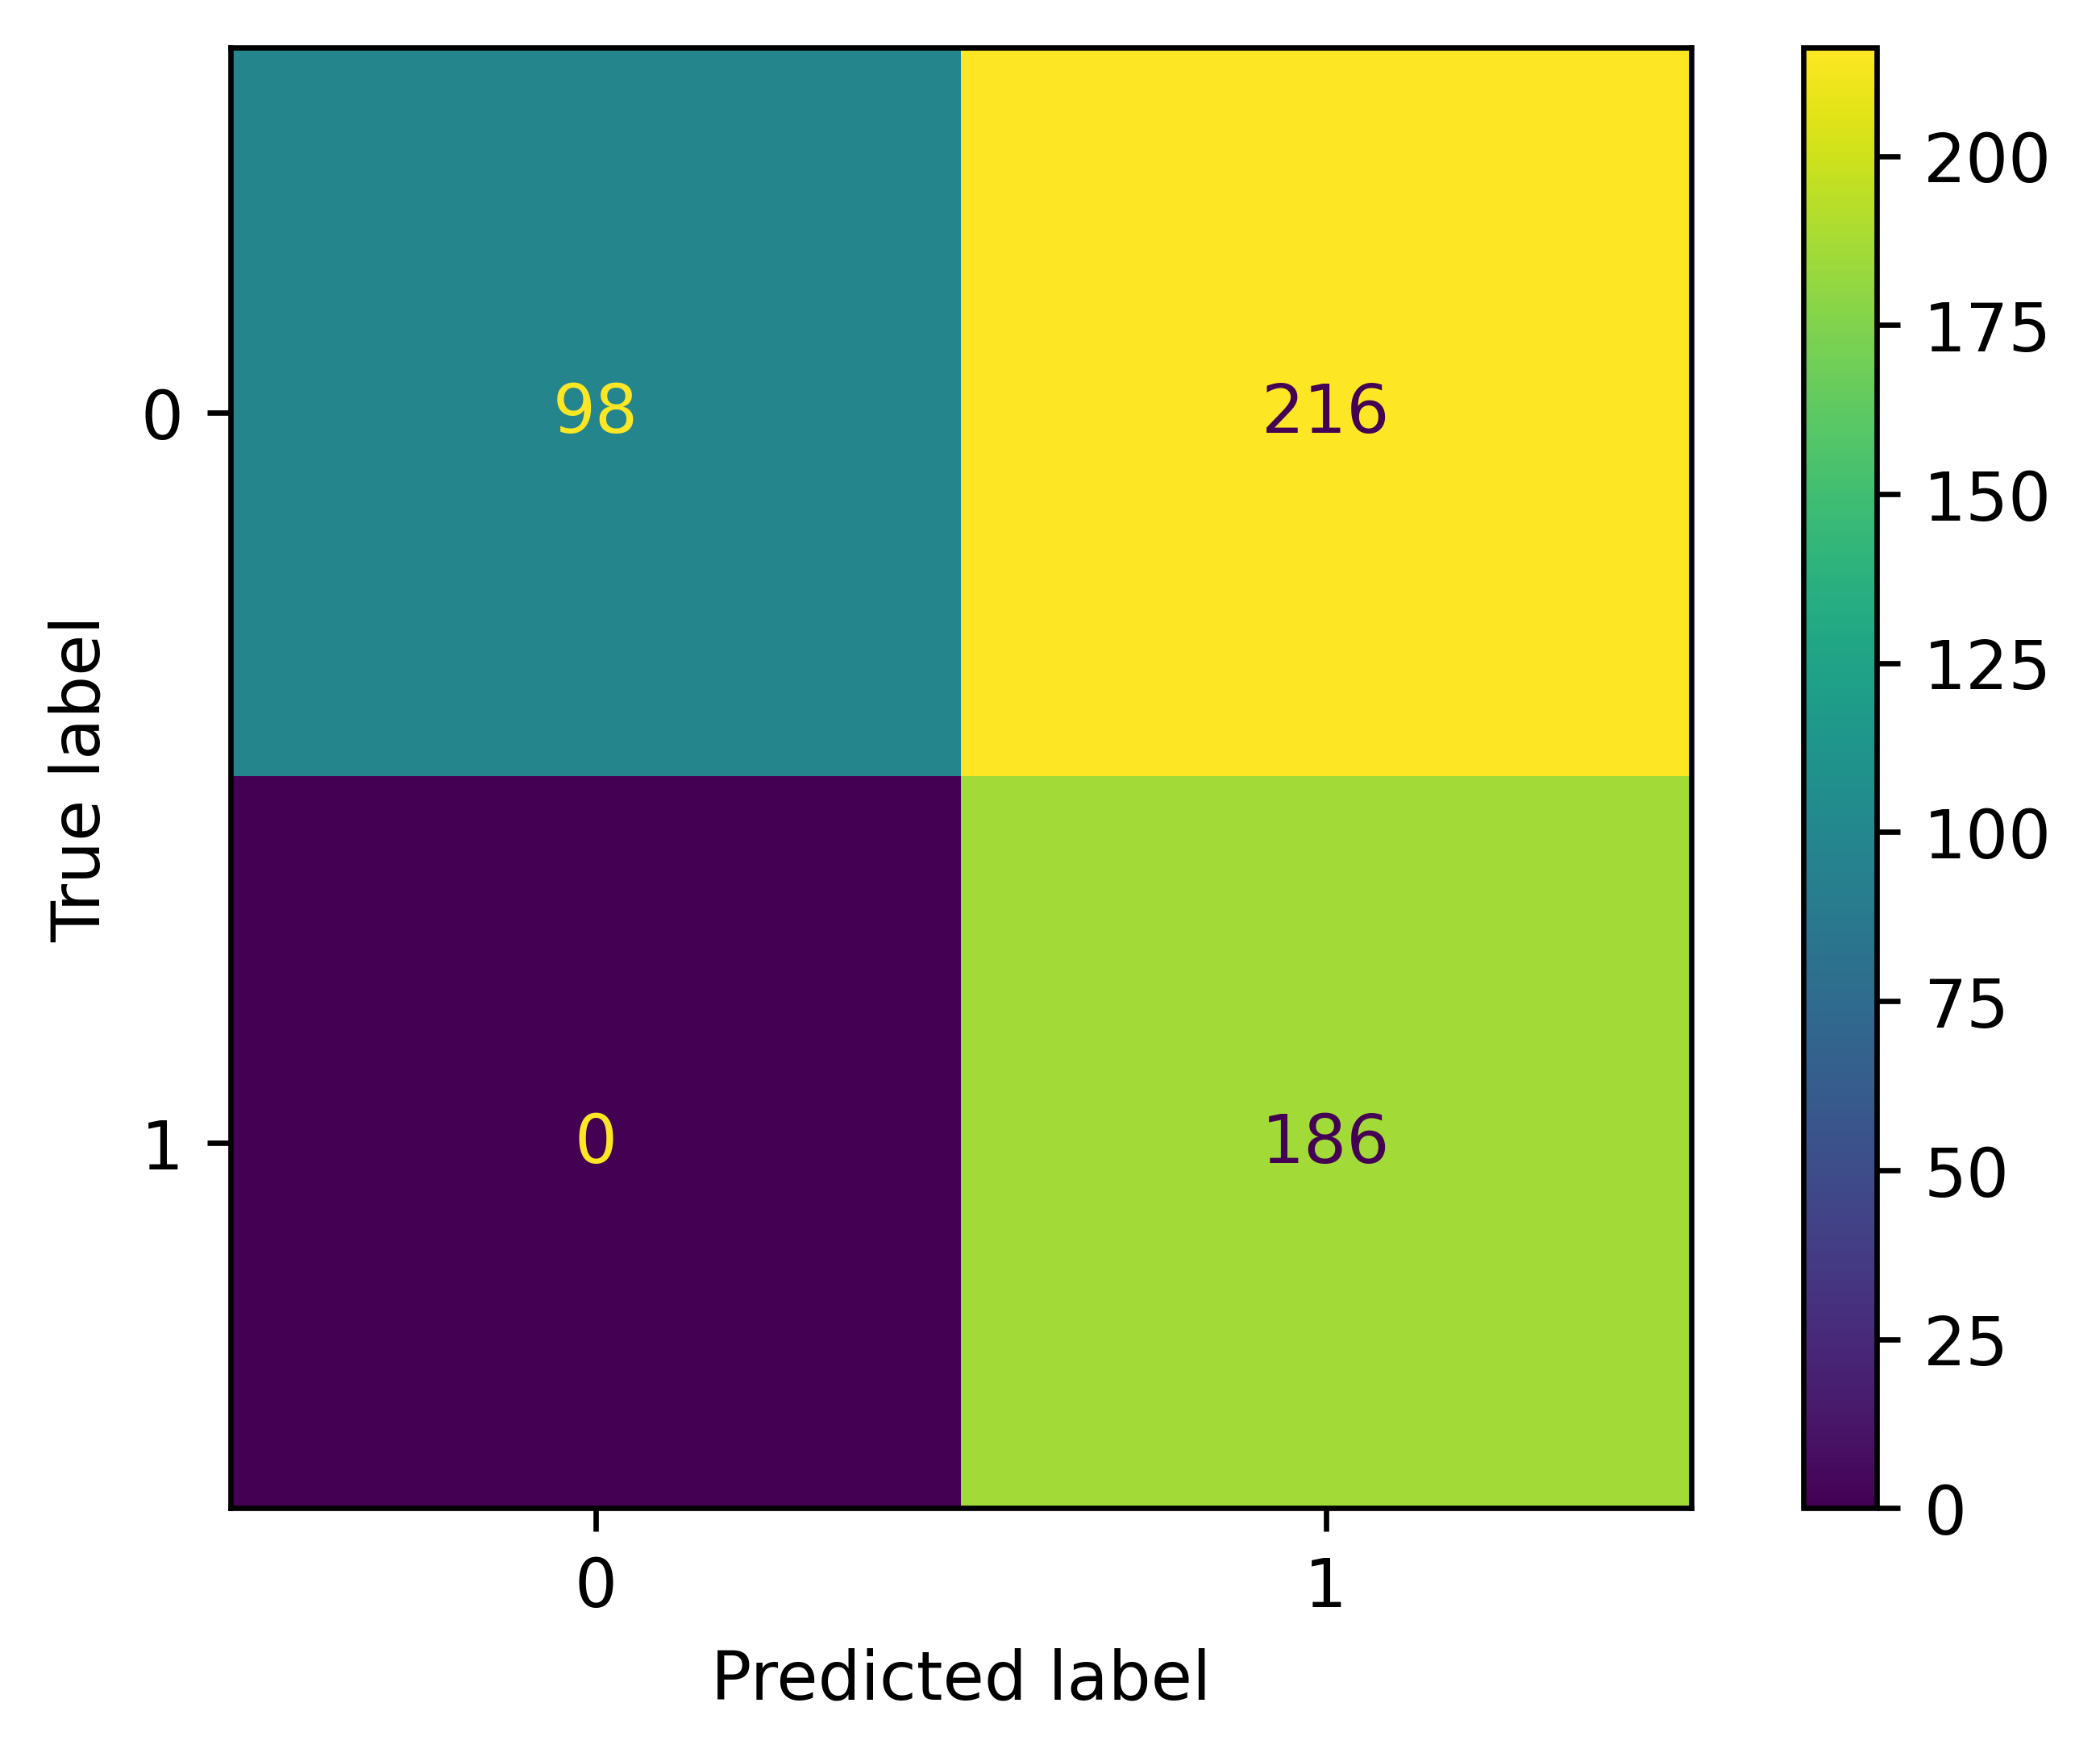
\includegraphics{Graphics/cm-th-06.png}}
	\subfigure[Curva ROC]{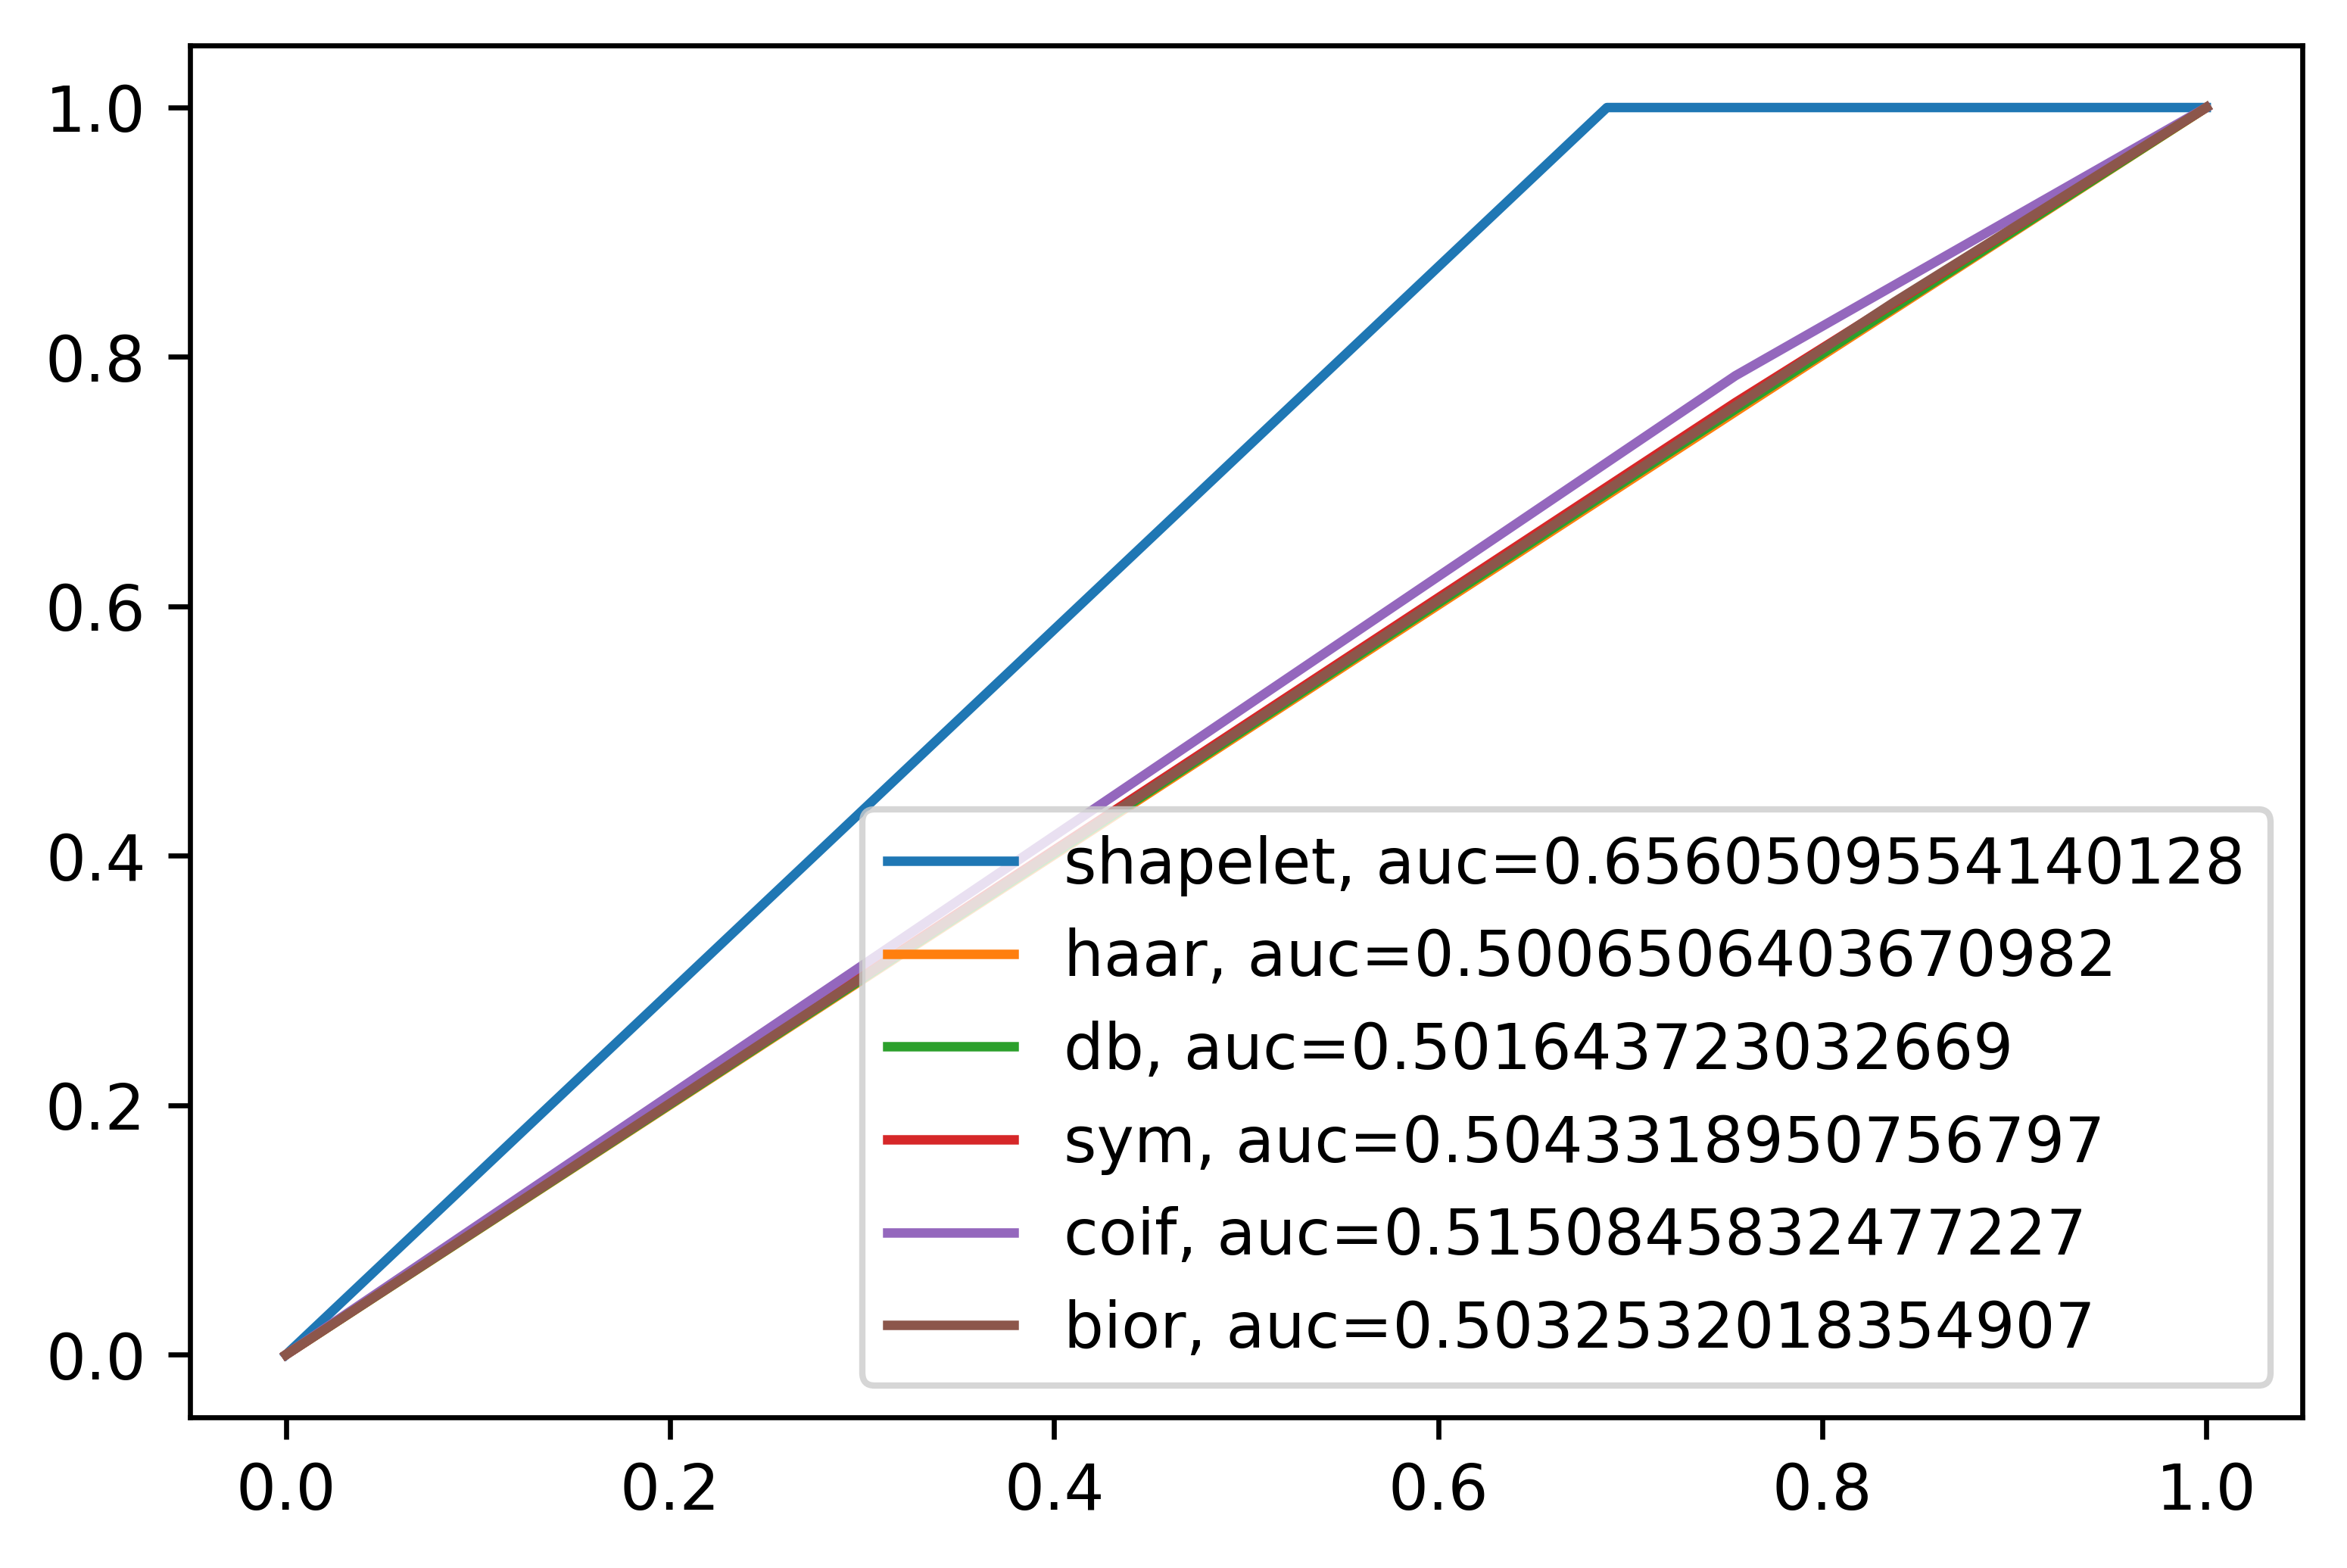
\includegraphics{Graphics/roc-th-06.png}}
	\caption{Matriz de confusión y curva ROC. En este ejemplo se tomó como umbral $th=0.60$} \label{fig:1d-experiment-060}
\end{figure}

\begin{figure}
	\centering
	\subfigure[Matriz de confusión]{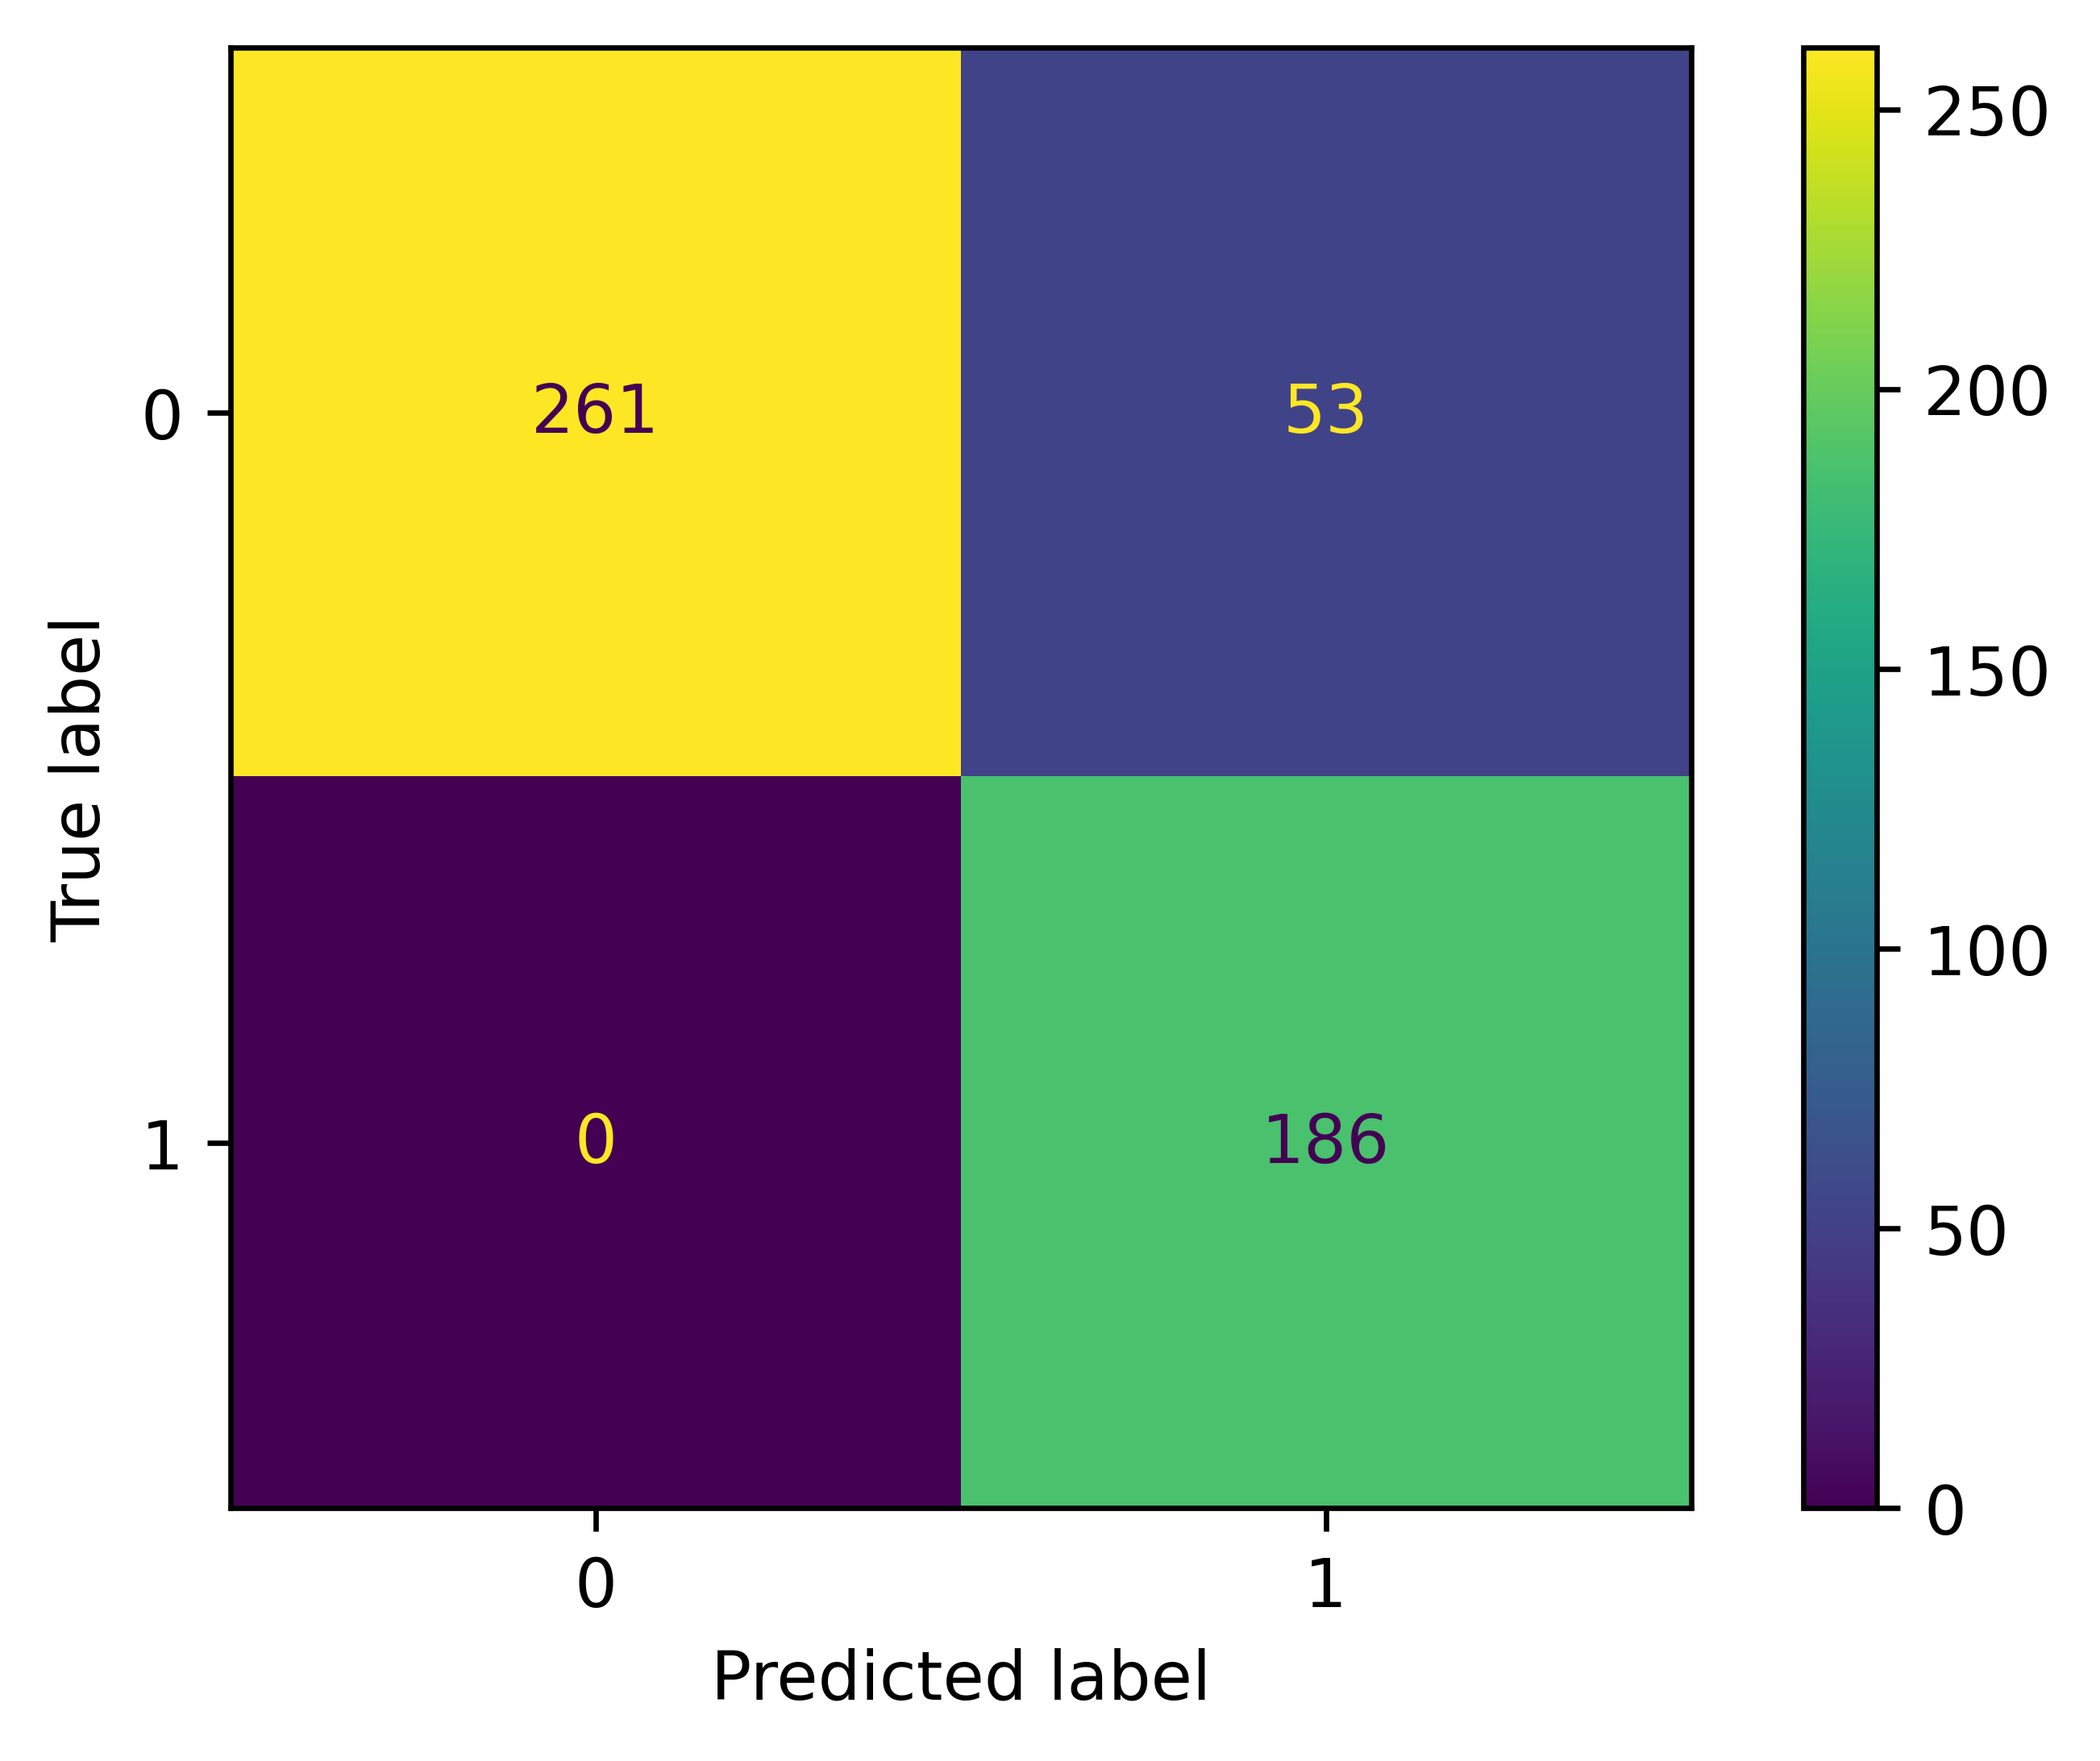
\includegraphics{Graphics/cm-th-085.png}}
	\subfigure[Curva ROC]{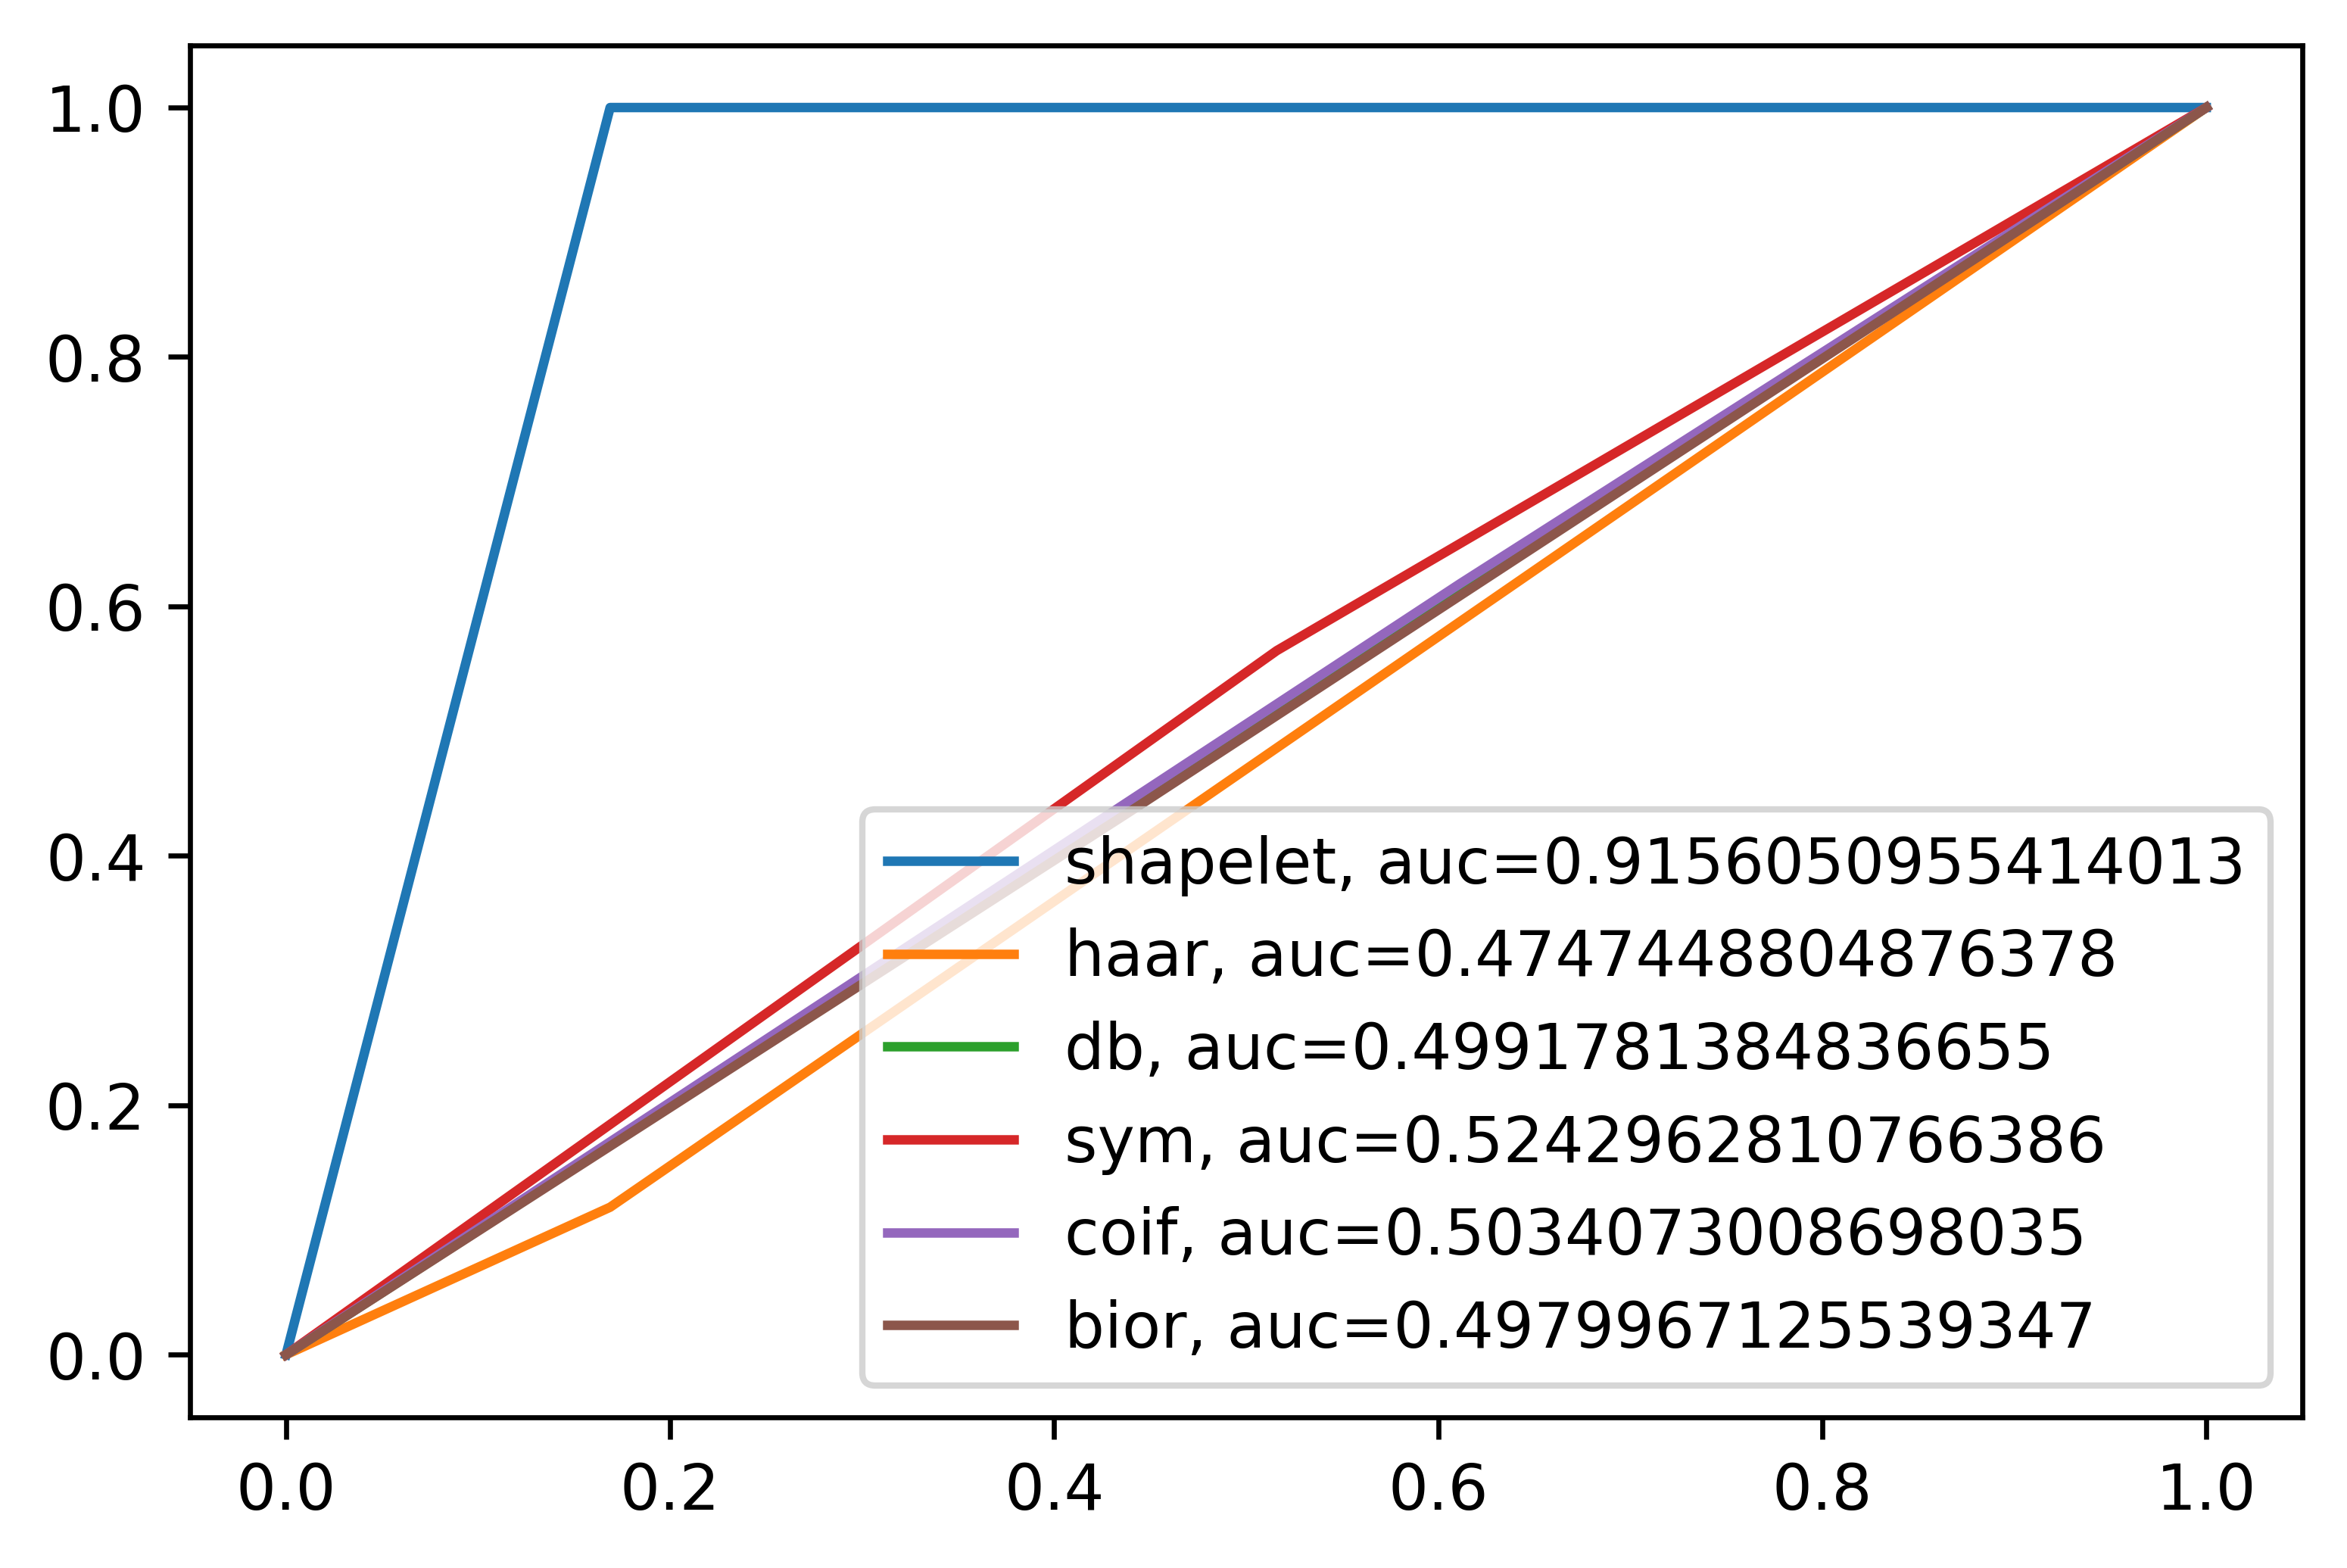
\includegraphics{Graphics/roc-th-085.png}}
	\caption{Matriz de confusión y curva ROC. En este ejemplo se tomó como umbral $th=0.85$} \label{fig:1d-experiment-085}
\end{figure}

\begin{figure}
	\centering
	\subfigure[Matriz de confusión]{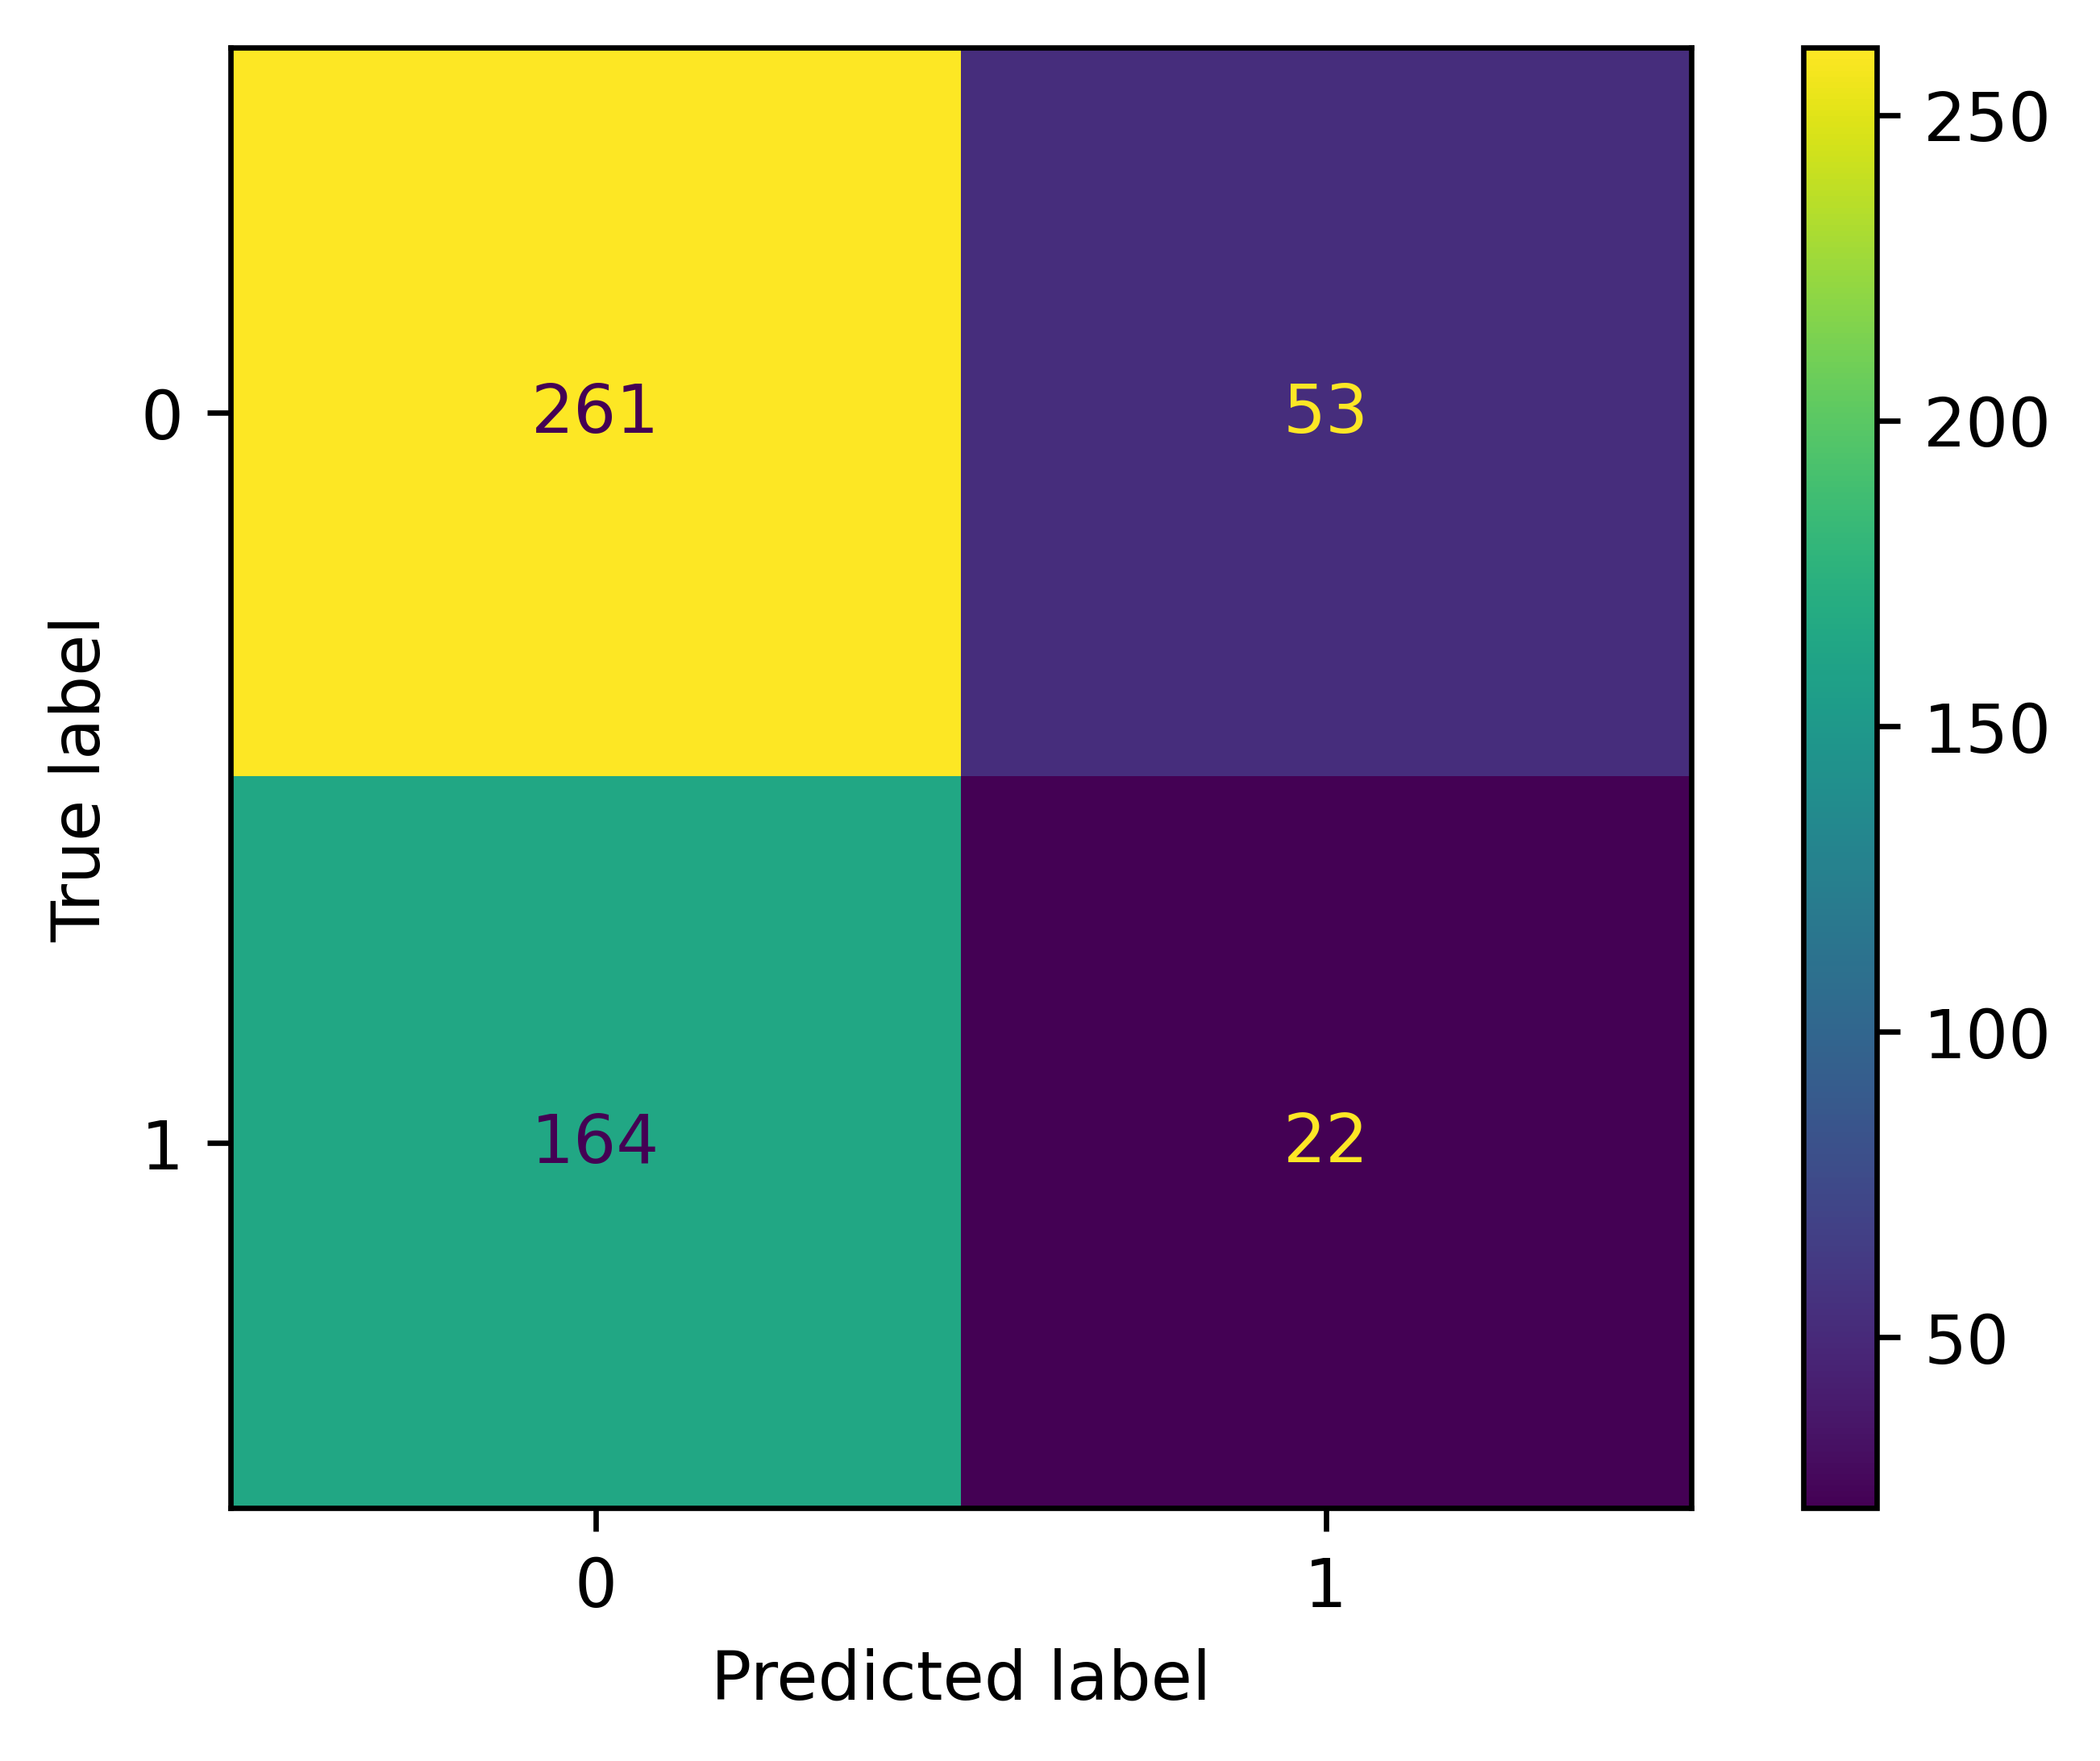
\includegraphics{Graphics/cm-th-098.png}}
	\subfigure[Curva ROC]{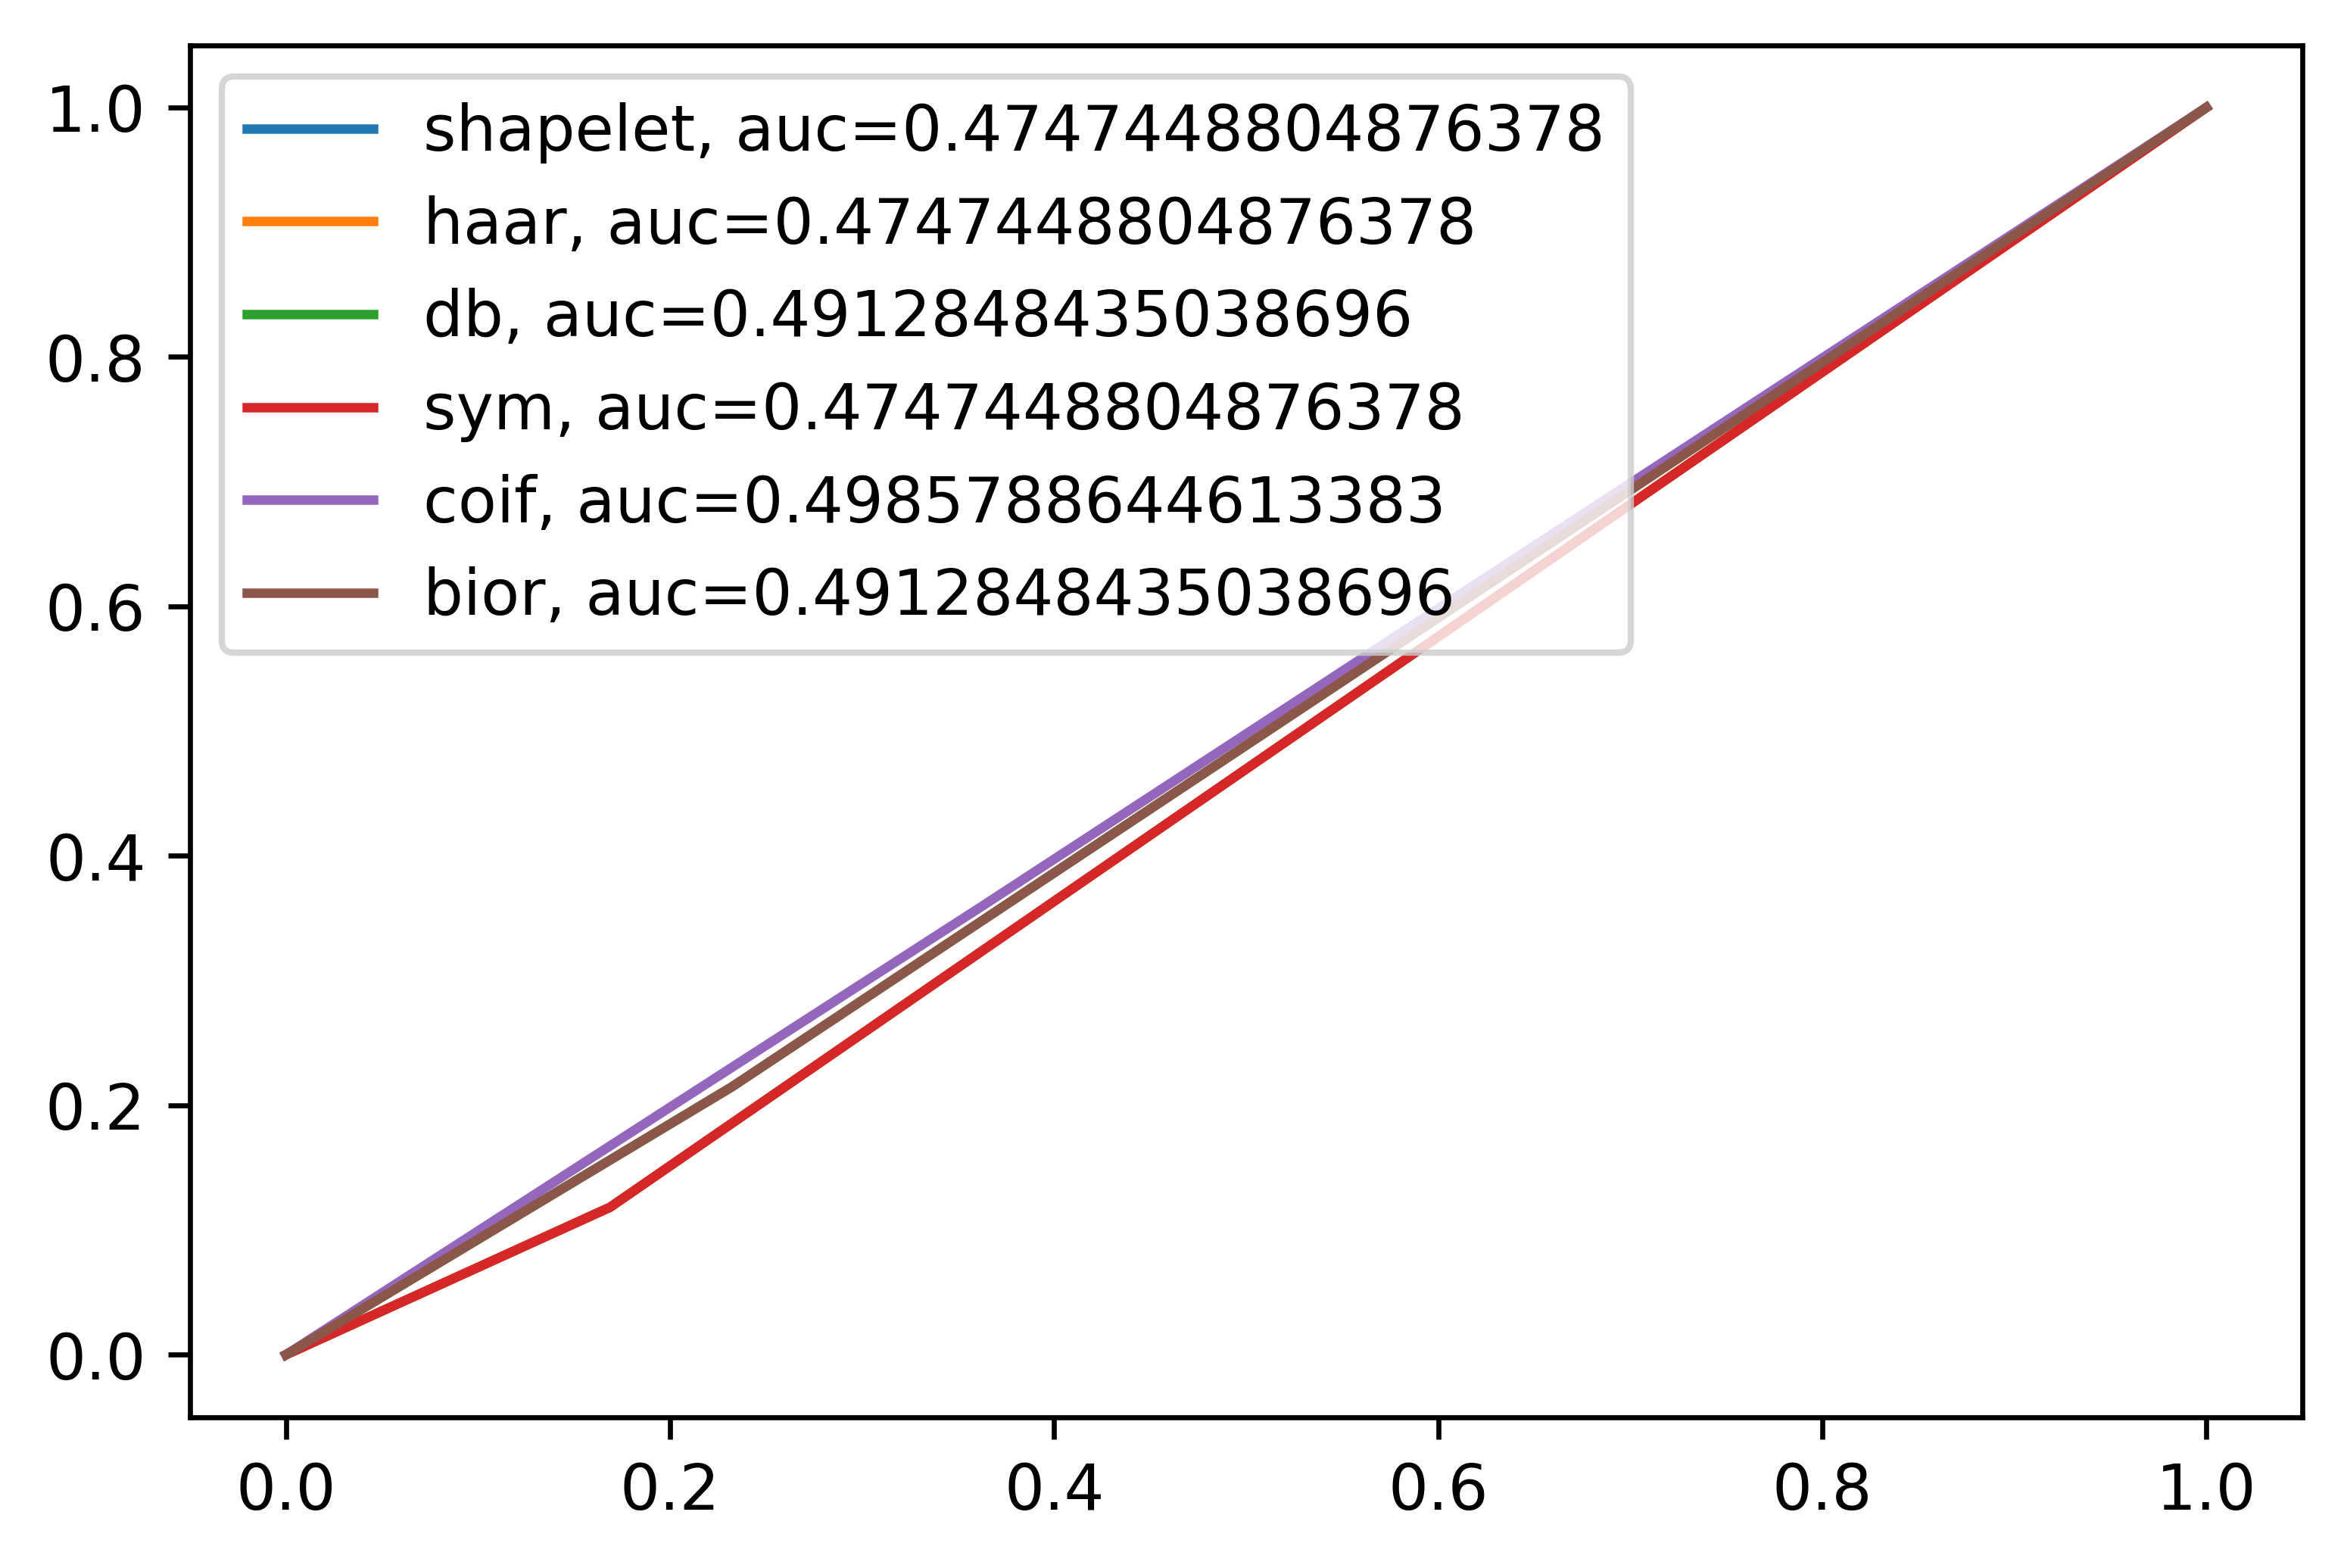
\includegraphics{Graphics/roc-th-098.png}}
	\caption{Matriz de confusión y curva ROC. En este ejemplo se tomó como umbral $th=0.98$} \label{fig:1d-experiment-098}
\end{figure}

Las figuras \ref{fig:1d-experiment-060},\ref{fig:1d-experiment-060} y \ref{fig:1d-experiment-098} muestran los resultados 
sobre el mismo conjunto de patrones y señales, pero variando el umbral $th$. El método numérico para la solución es el
mismo: Levenberg-Marquardt.

Seleccionando un umbral $th=0.6$, permite al algoritmo sacarle provecho a su capacidad de detectar el patrón. Sin embargo,
sigue habiendo una gran cantidad de falsos positivos. Si se aumenta este umbral a $th=0.85$ se puede que este número
disminuye considerablemente, pues de 216 pasa a ser tan solo 53. Como consecuencia de esto el área debajo de la curva
(\textit{auc}) llega a alcanzar $0.90$, lo cual es un resultado sumamente bueno para un clasificador binario.

Si se sigue aumentando el umbral, esta vez a $0.98$, los resultados cambian drásticamente. La \textit{shapelet} no
se comporta para nada distinto al resto de las wavelets. Aunque teóricamente un valor igual a cero en $S$ indica
la detección exacta del patrón, siempre existe un erro durante el cálculo del filtro $q$ que impide que esto sea
cierto en la práctica. Por este motivo, poner el umbral de detección demasiado alto empeora los resultados.
Por lo tanto un valor entre $0.6$ (valor q recomiendan en \cite{Guido2018}) y $0.90$ se considera idóneo.

\section{Detección de patrones en señales 2D}

Una vez evaluado la capacidad de la replicación de la DST-II, se procede a la exploración de sus capacidades 
para el caso de señales 2D. A continuación se describen en detalles de los experimentos y resultados.

Para llevar a cabo la experimentación se crearon imágenes artificiales con figuras simples. Entre ellas se incluyen gaussianas,
círculos y zonas rectangulares. El objetivo es evaluar la capacidad del algoritmo para detectar en el caso de 2D
y su sensibilidad ante el ruido. Sobre cada una de estas figuras se utilizó cada una de las propuestas de \ref{section:2d}.
El resultado se evaluaba visualmente, sobre el  mapa de colores \ref{fig:colormap} donde valores mayores son más cercanos
al amarillo y menores al azul.

\begin{figure}
	\centering
	
\includegraphics[scale=0.8]{Graphics/colormap.png} 
	\caption{Mapa de colores usado para evaluar la detección de la DST-II. Valores pequeños son representados en tonalidades azules y valores altos en amarillo} \label{fig:colormap}
\end{figure}

\subsection{Ejemplos de los experimentos y análisis de los resultados}

\begin{figure}
	\centering
	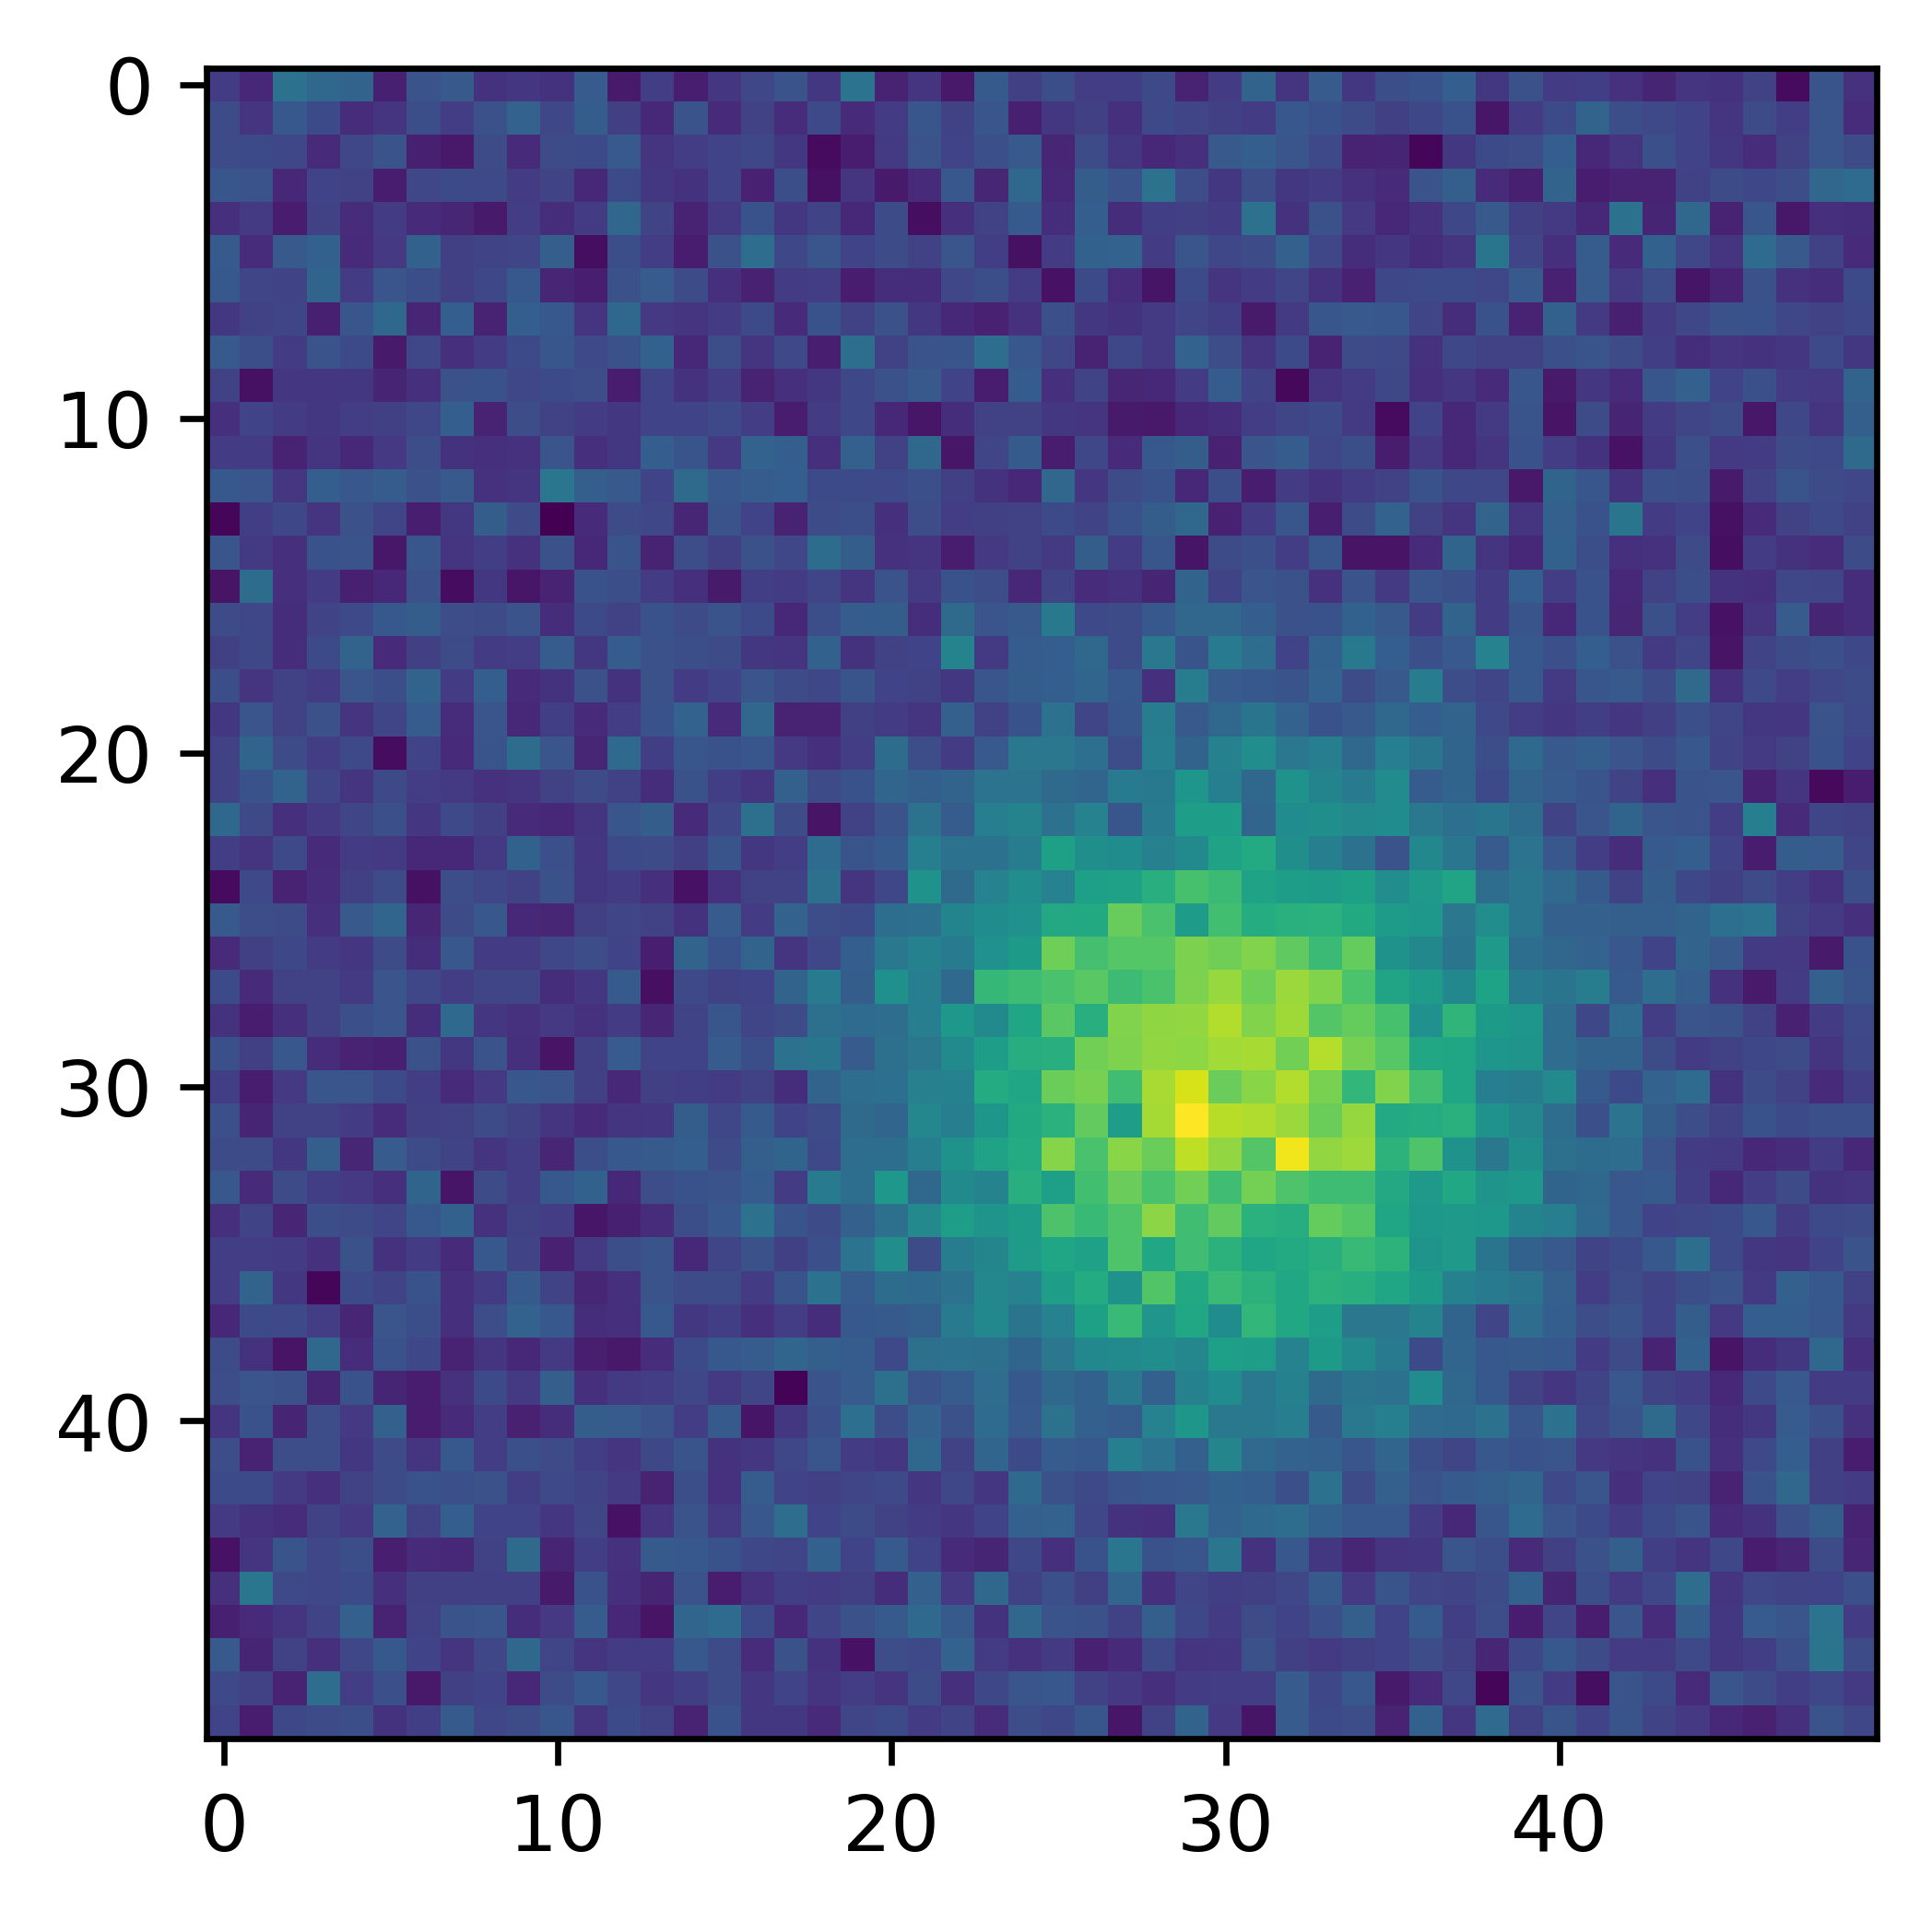
\includegraphics{Graphics/gaussian-2d-experiment.png}
	\caption{Gaussiana centrada en la posición (30,30)} \label{fig:gaussian-example-experiment}
\end{figure}

\begin{figure}
	\centering
	\subfigure[Sección horizontal]{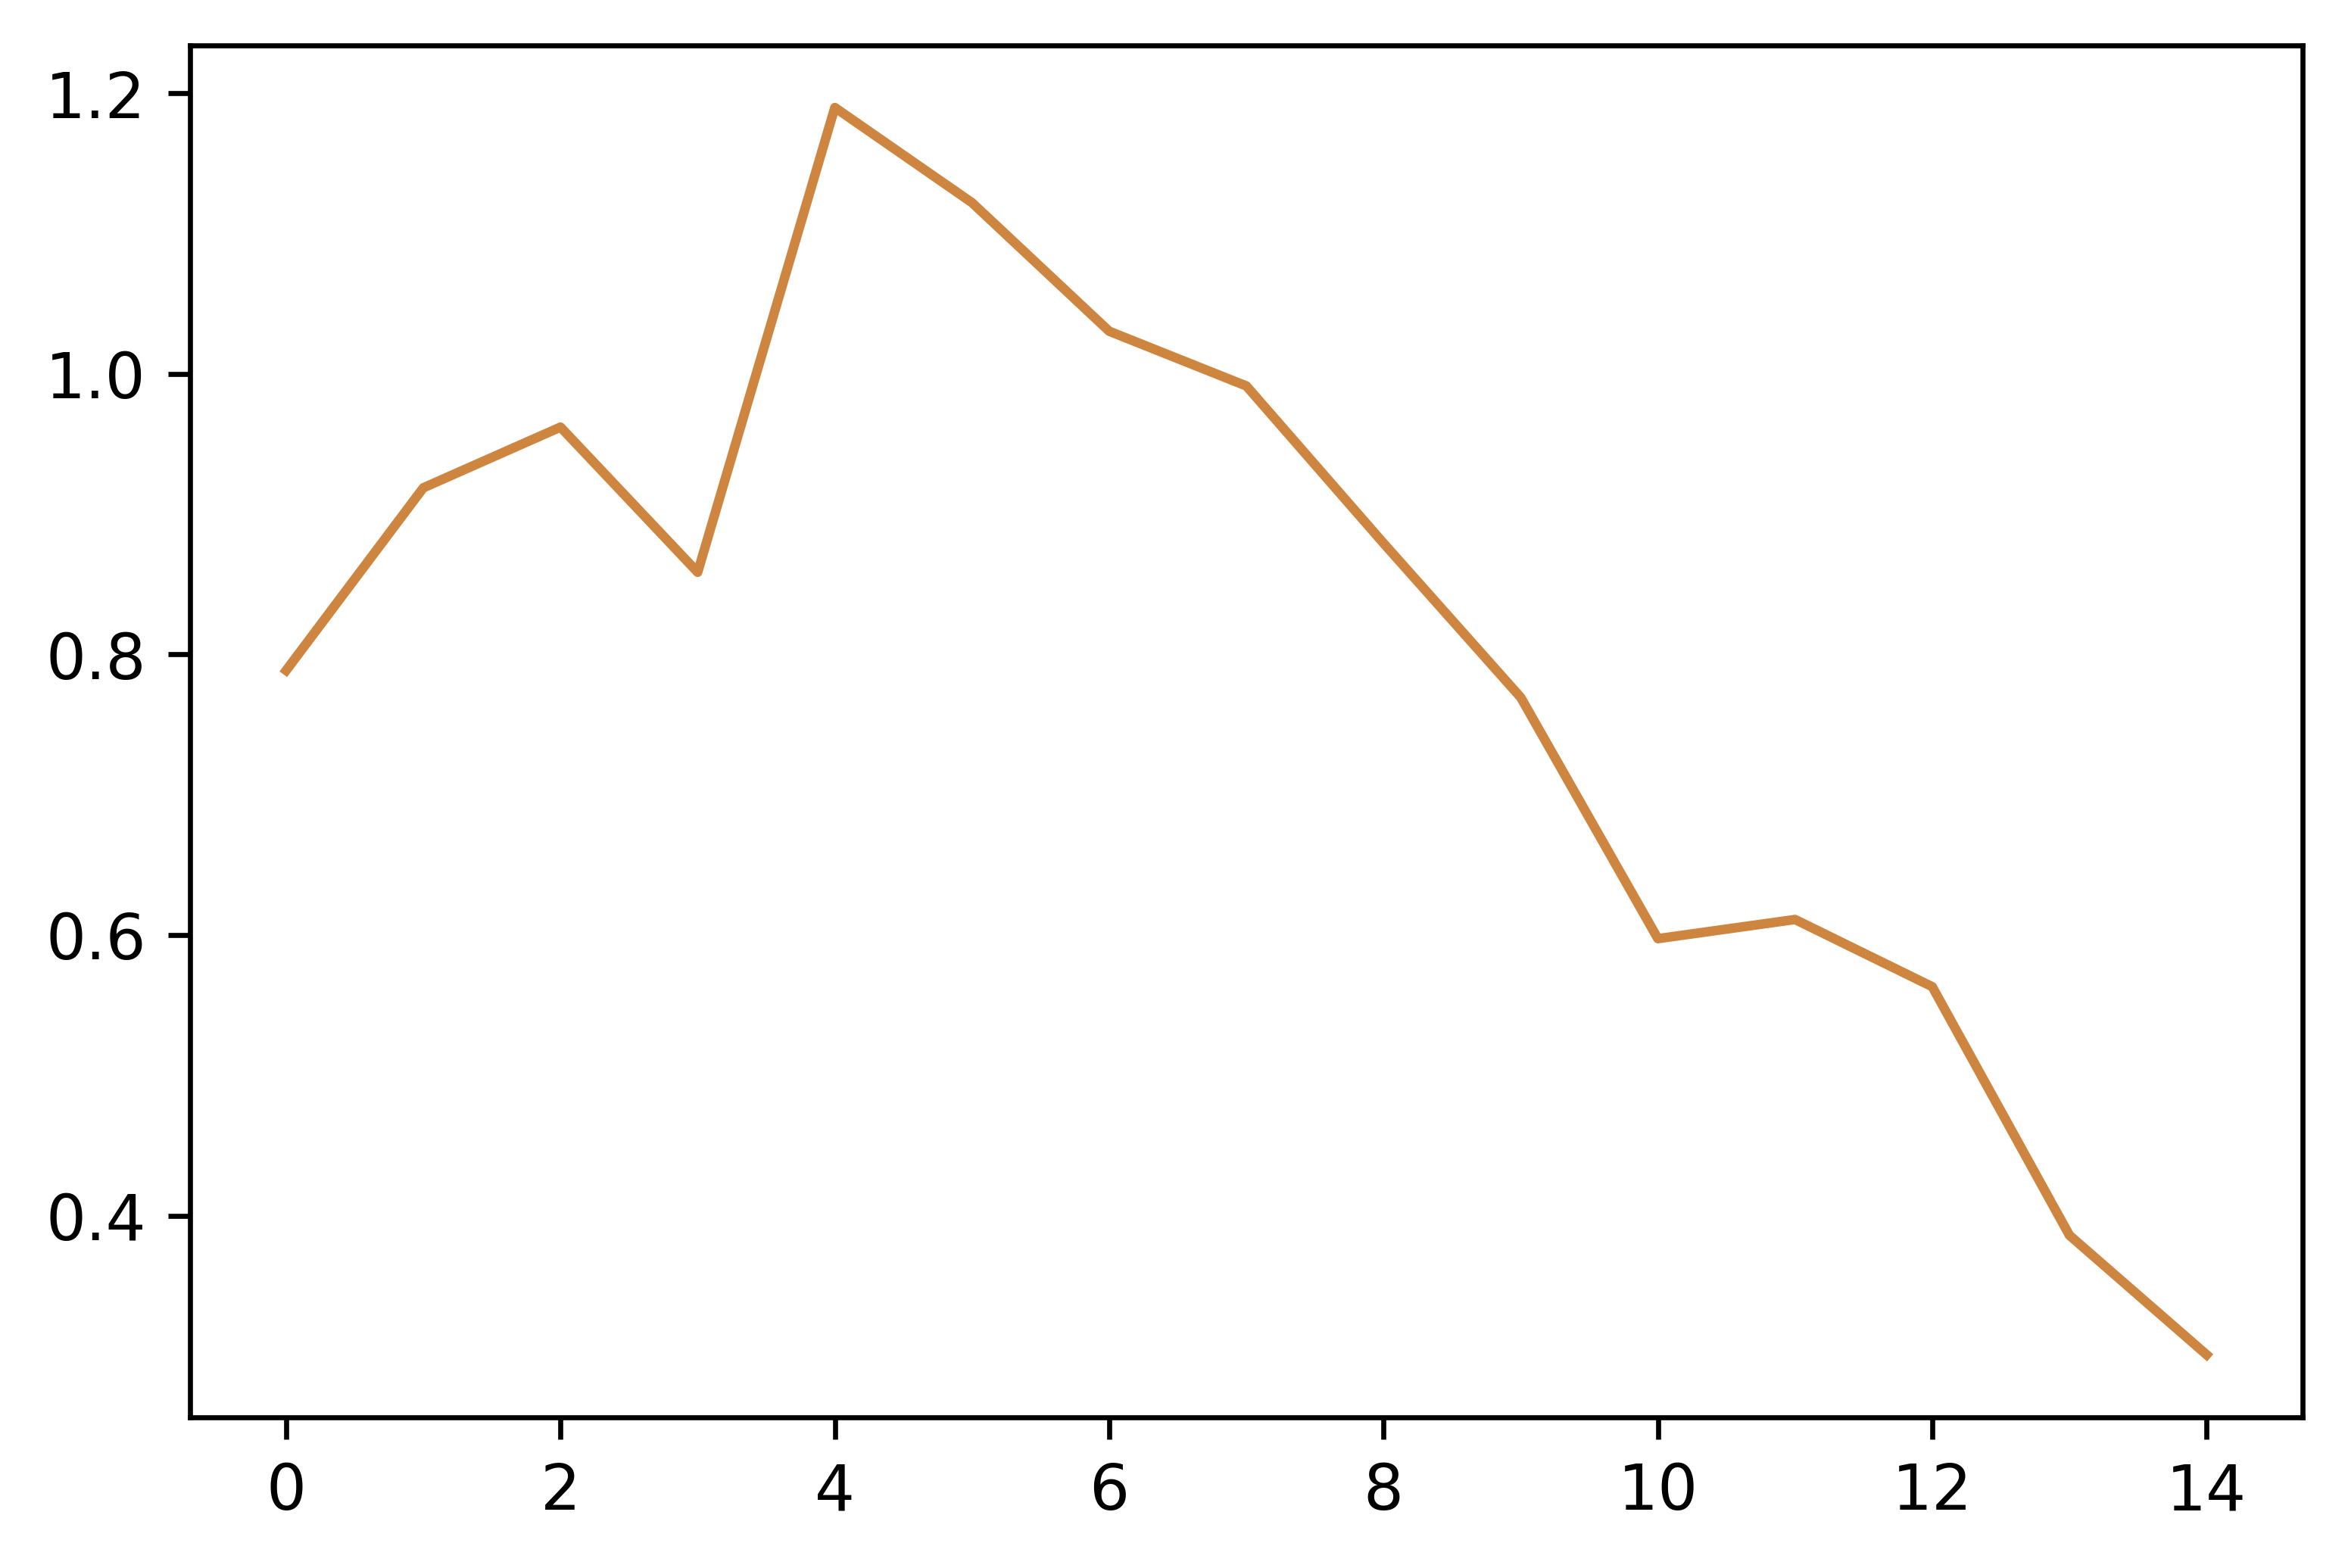
\includegraphics{Graphics/line-gaussian-experiment.png}}
	\subfigure[Sección vertical]{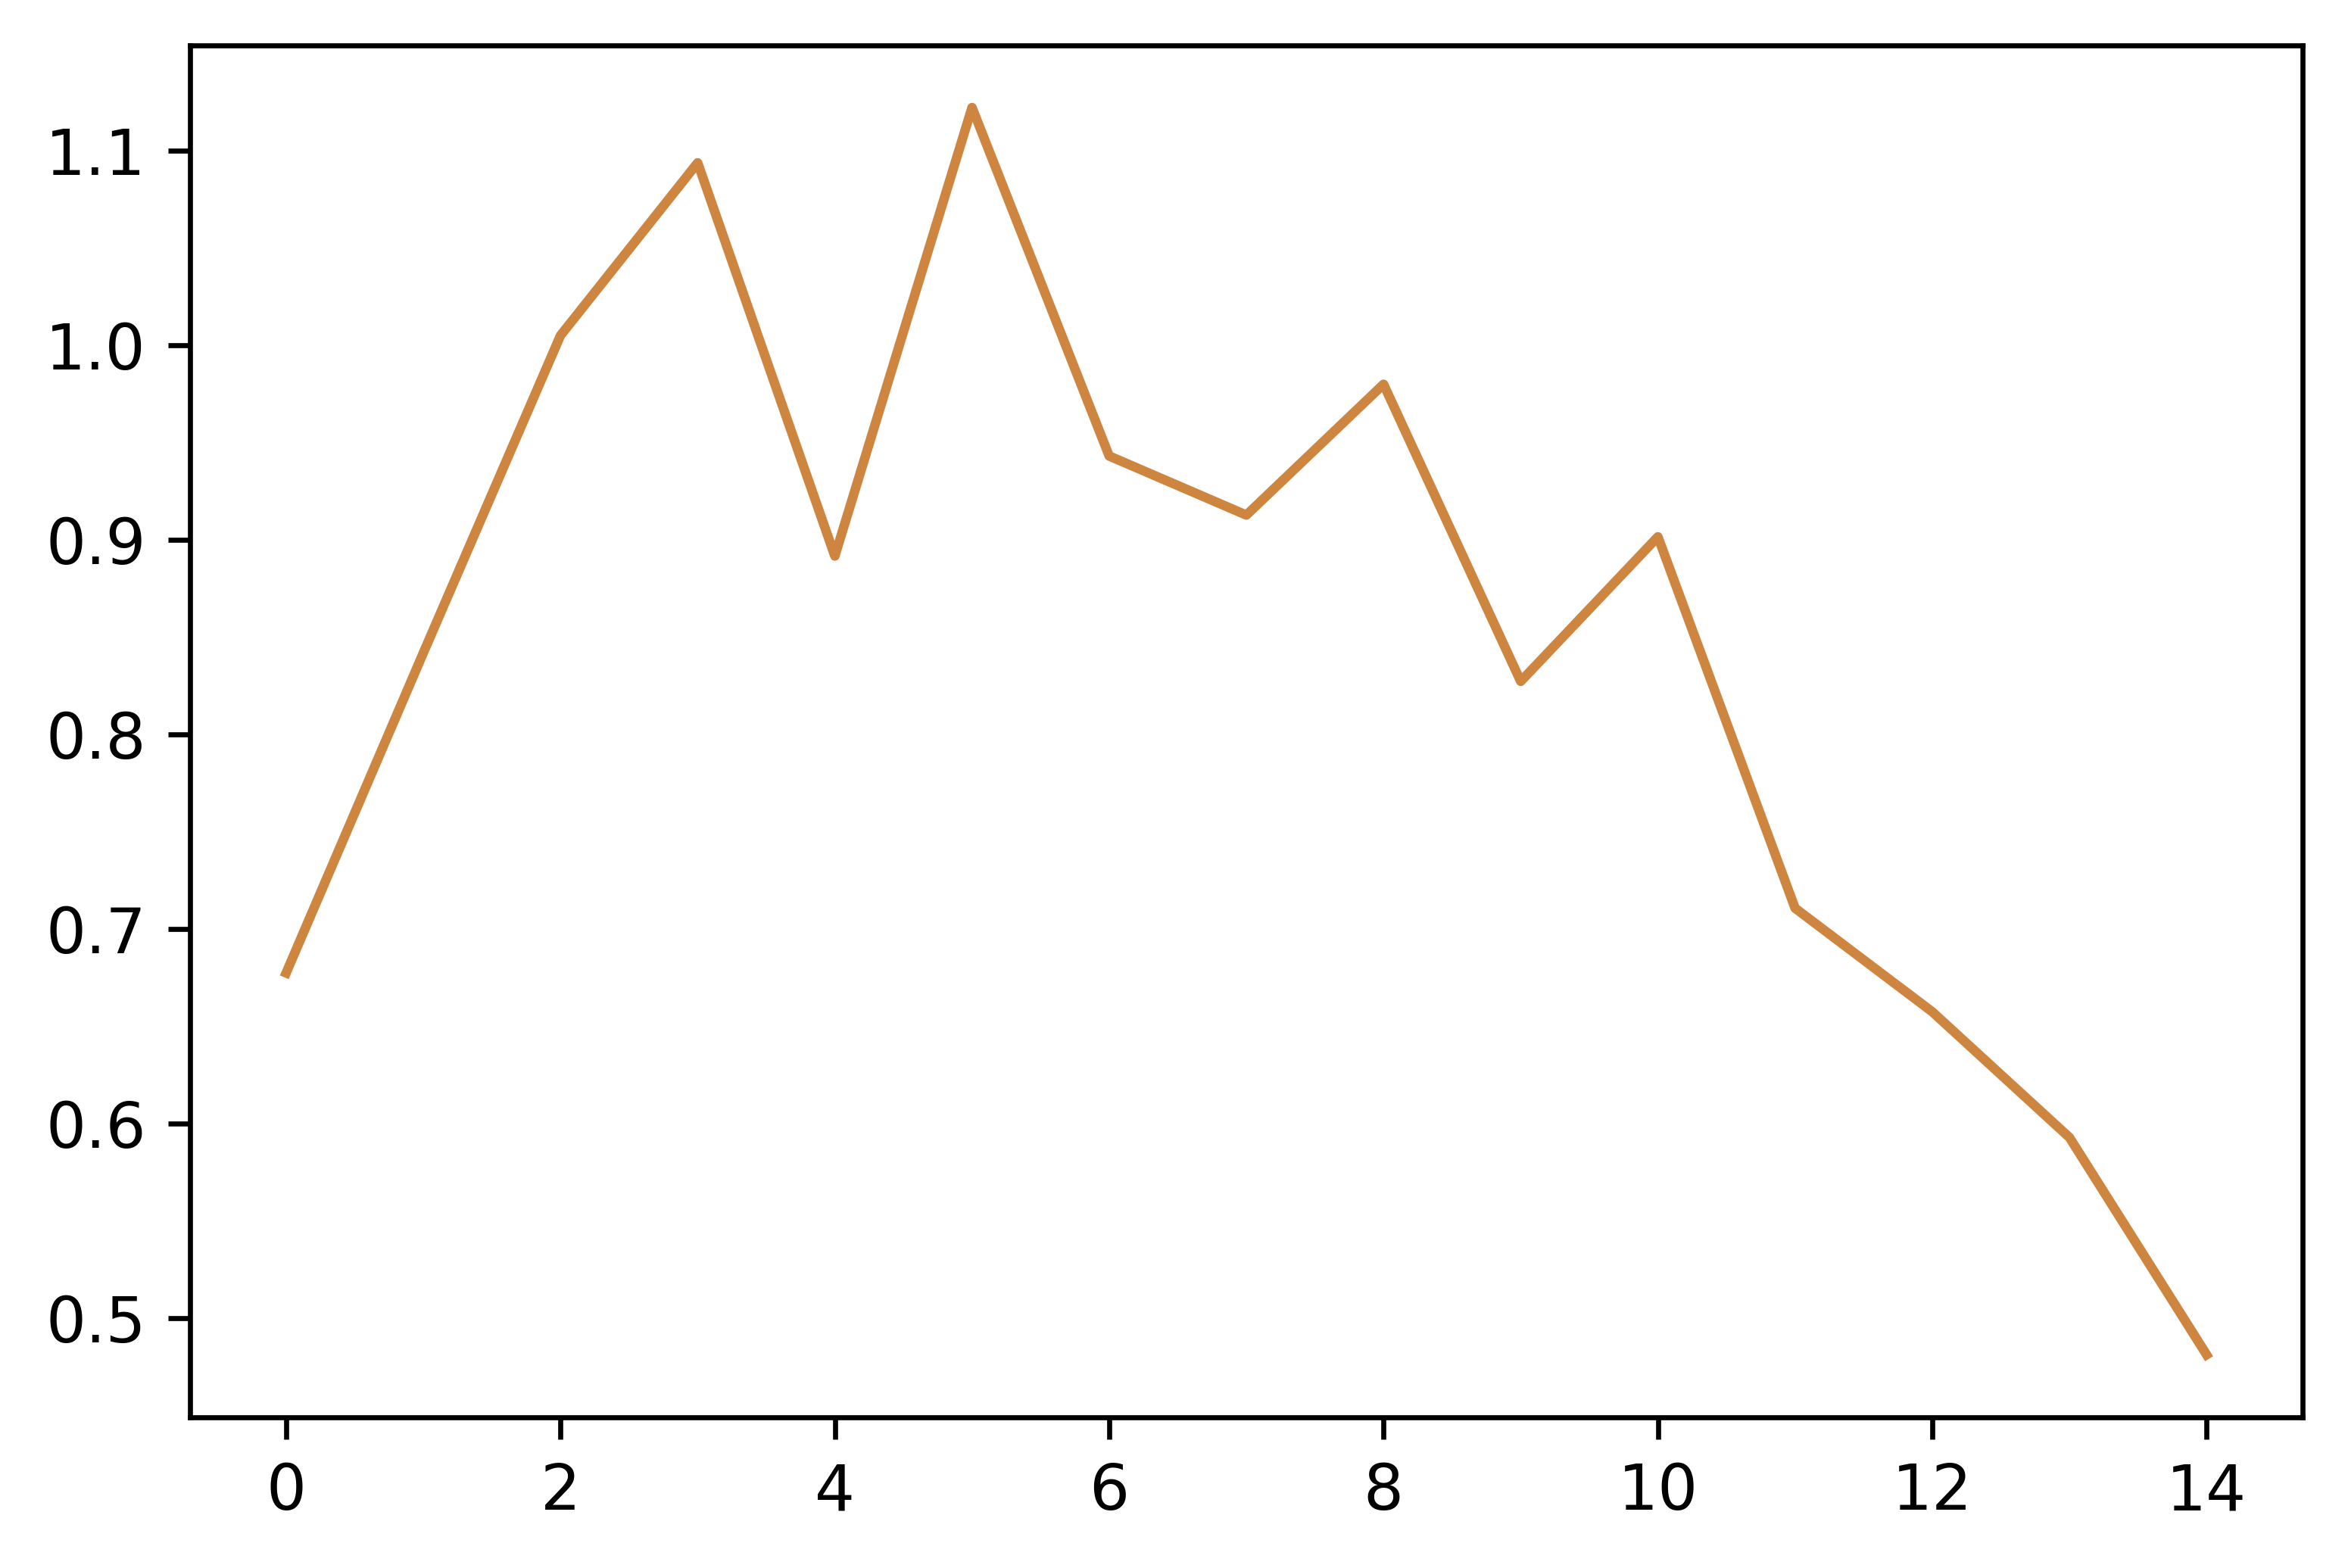
\includegraphics{Graphics/line-gaussian-experiment-vertical.png}}
	\caption{ Secciones correspondientes a [30,25:40] y [25:40,30] de \ref{fig:gaussian-example-experiment}} \label{fig:lines-experiment}
\end{figure}

Como ejemplo se toma la imagen \ref{guassian-example-experiment}. Siguiendo el primer enfoque se toman las secciones
\ref{fig:lines-experiment} y se construyen dos shapelets obteniendose cutro componentes como resultado de la 
transformada. La figura \ref{fig:gaussian-example-approach1} muestra el resultado. Como se puede apreciar, en ninguno de 
los coeficientes se obtiene un contraste alto con el resto, y de hecho ninguno supera el valor de $S(c)=0.8$.

Esto se debe a que las ecuaciones de \textit{matching} \ref{eq:matching-1} \ref{eq:matching-2} están 
construidas para que la convolución entre el la sección de la señal que se parece al patrón y 
el filtro sea lo más cercano a cero en el coeficiente más cercano que corresponde a la posición donde está el patrón.
Sin embargo, como se explica en \ref{section:dwt-2d}, primero se realiza la transformada sobre las filas y luego al resultado
se le realiza nuevamente la transformada, pero en las columnas. 

En el caso de la primera transformada la detección es posible y funciona de igual forma que si fuera una señal
unidimensional, solo que ahora se realiza por pedazos ( las filas ). 
Pero una vez que se pasa a la segunda transformada sobre las columnas, las condiciones para la detección del patrón no se cumplen.
Las ecuaciones \ref{eq:matching-1} \ref{eq:matching-2} están diseñadas para que la convolución sea lo más cercana a cero
solamente si se está pasando el filtro sobre los valores del patrón, no sobre su transformada.

Esto limita la extensión de las capacidades de detección de la DST-II para señales de más de una dimension tal y como se puede
aprecia en el ejemplo anterior. Resultados similares se obtuvieron en otros ejemplos. Por lo tanto, esta no es una 
vía factible para extender la DST-II para señales bidimensionales.


\begin{figure*}
\begin{multicols}{2}
    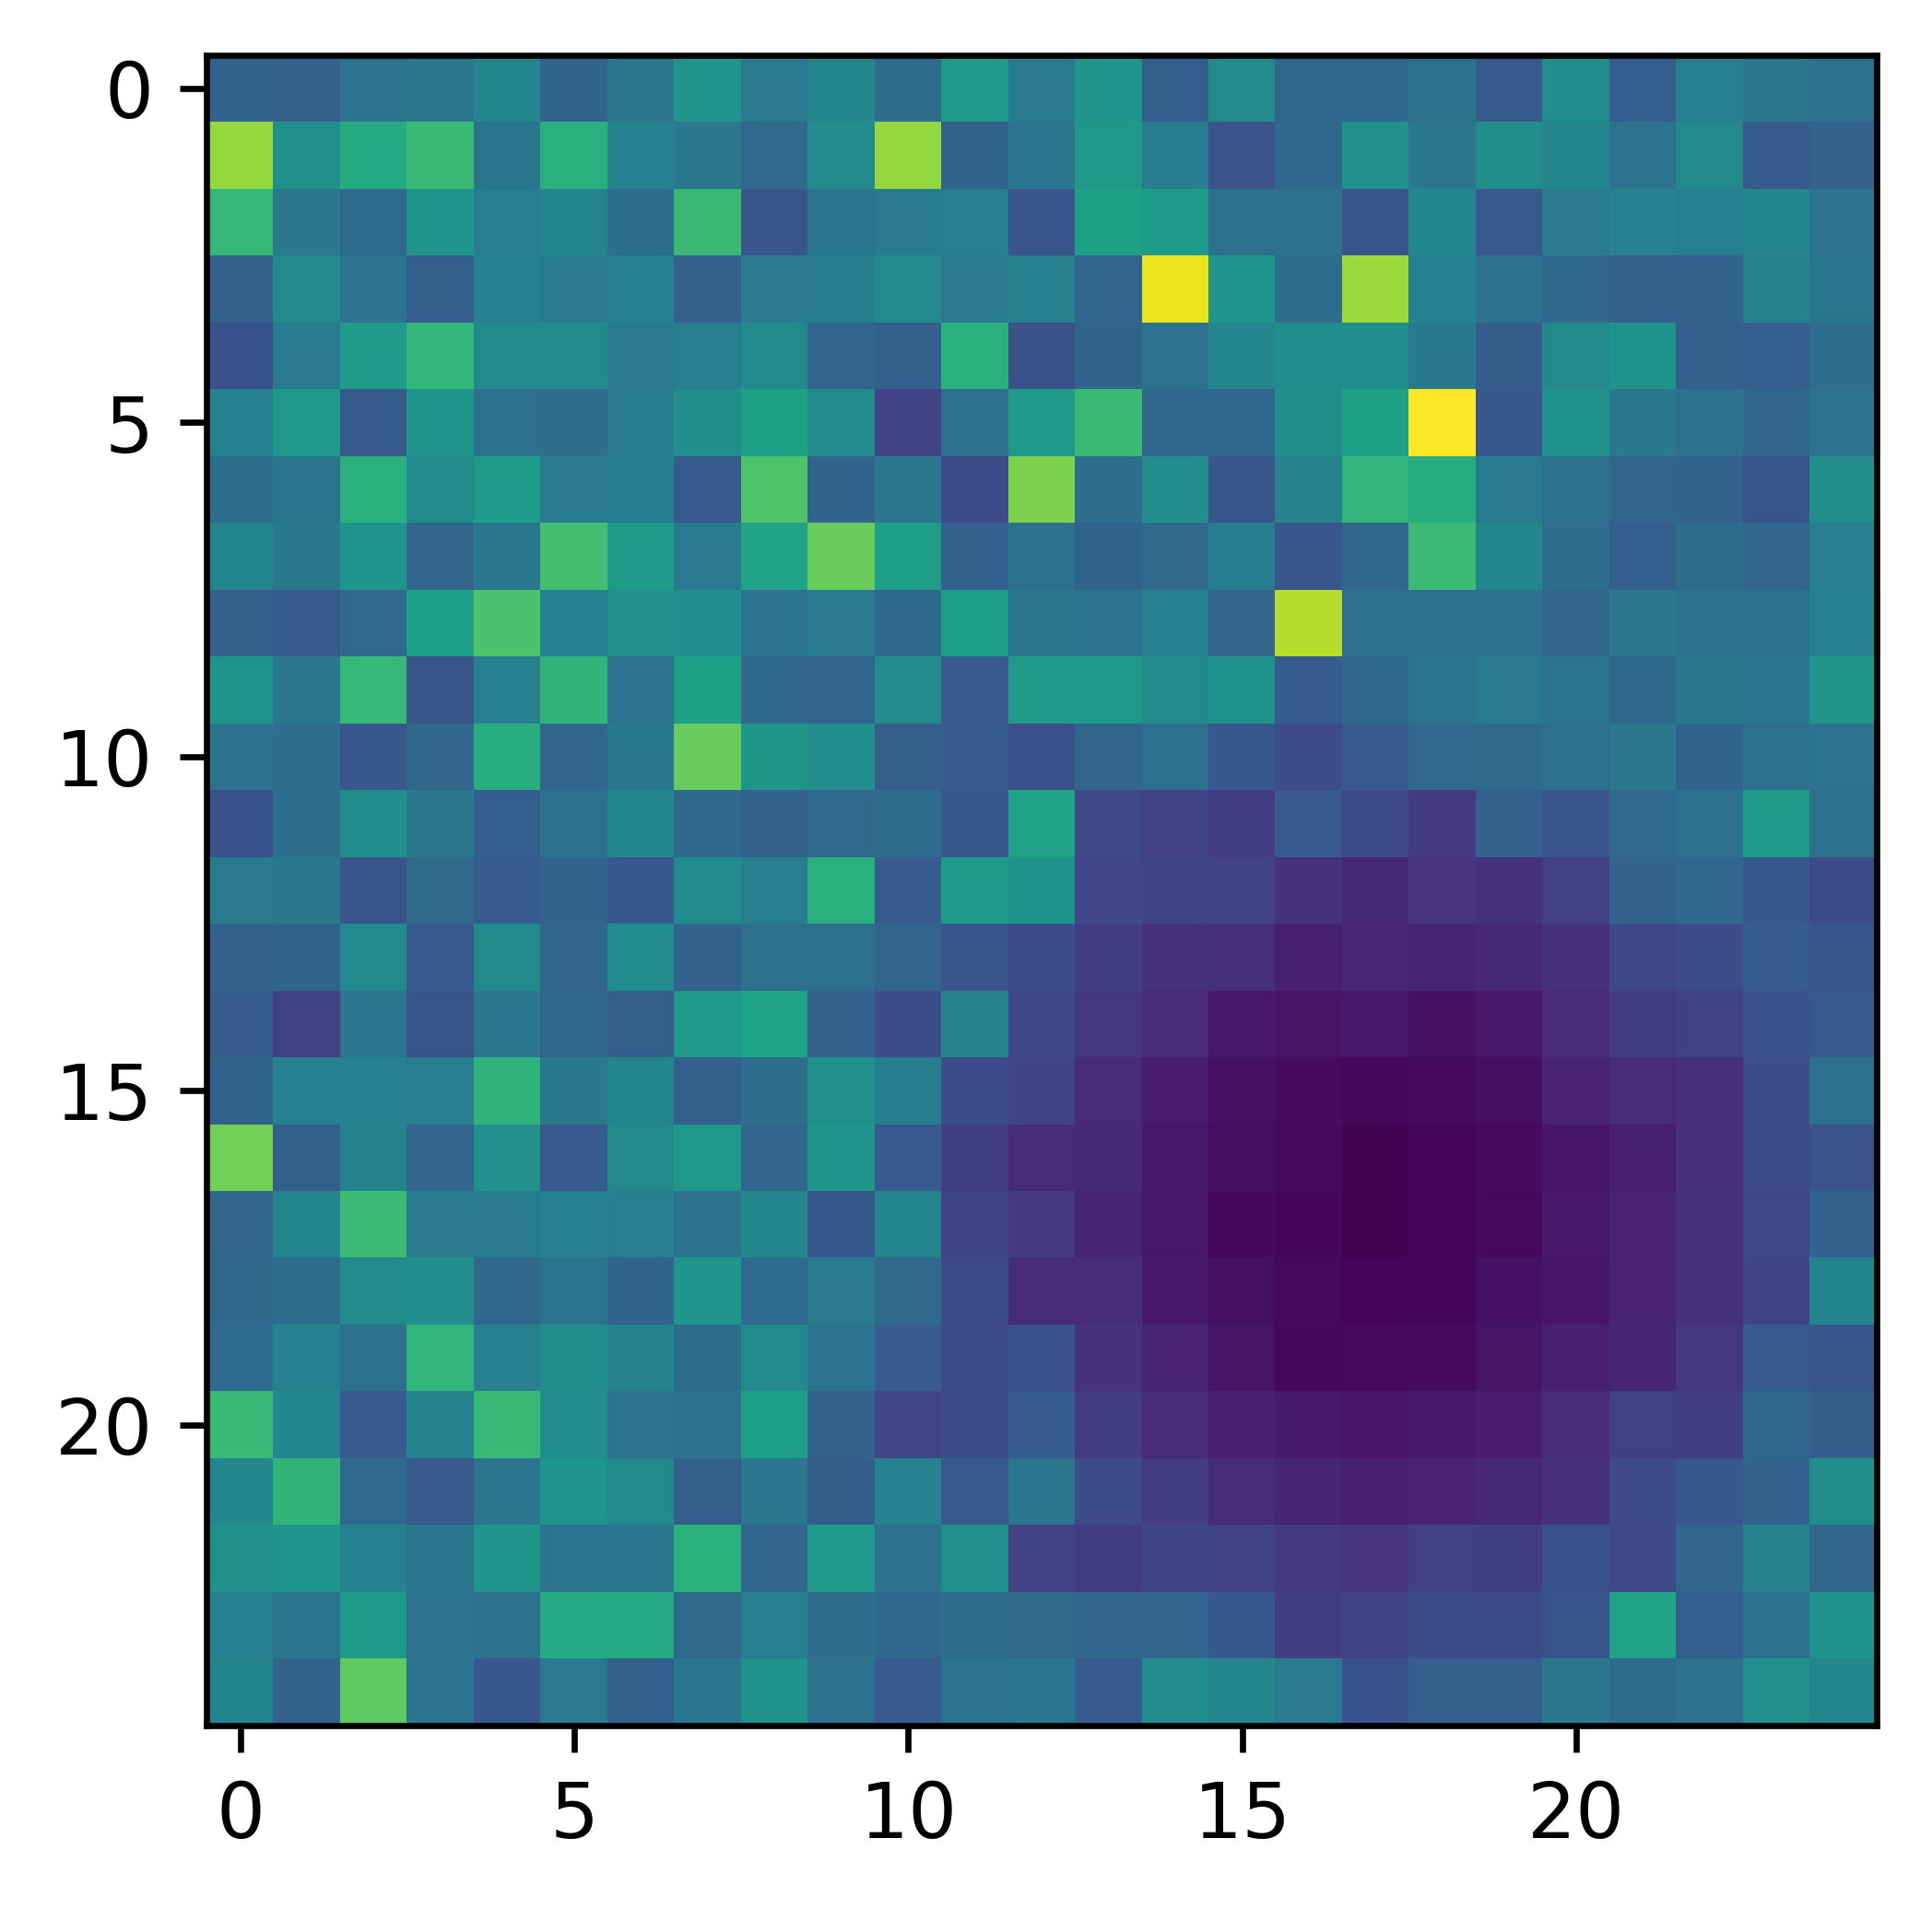
\includegraphics[width=\linewidth]{Graphics/guassian-2d-experiment-aprox.png}\par 
    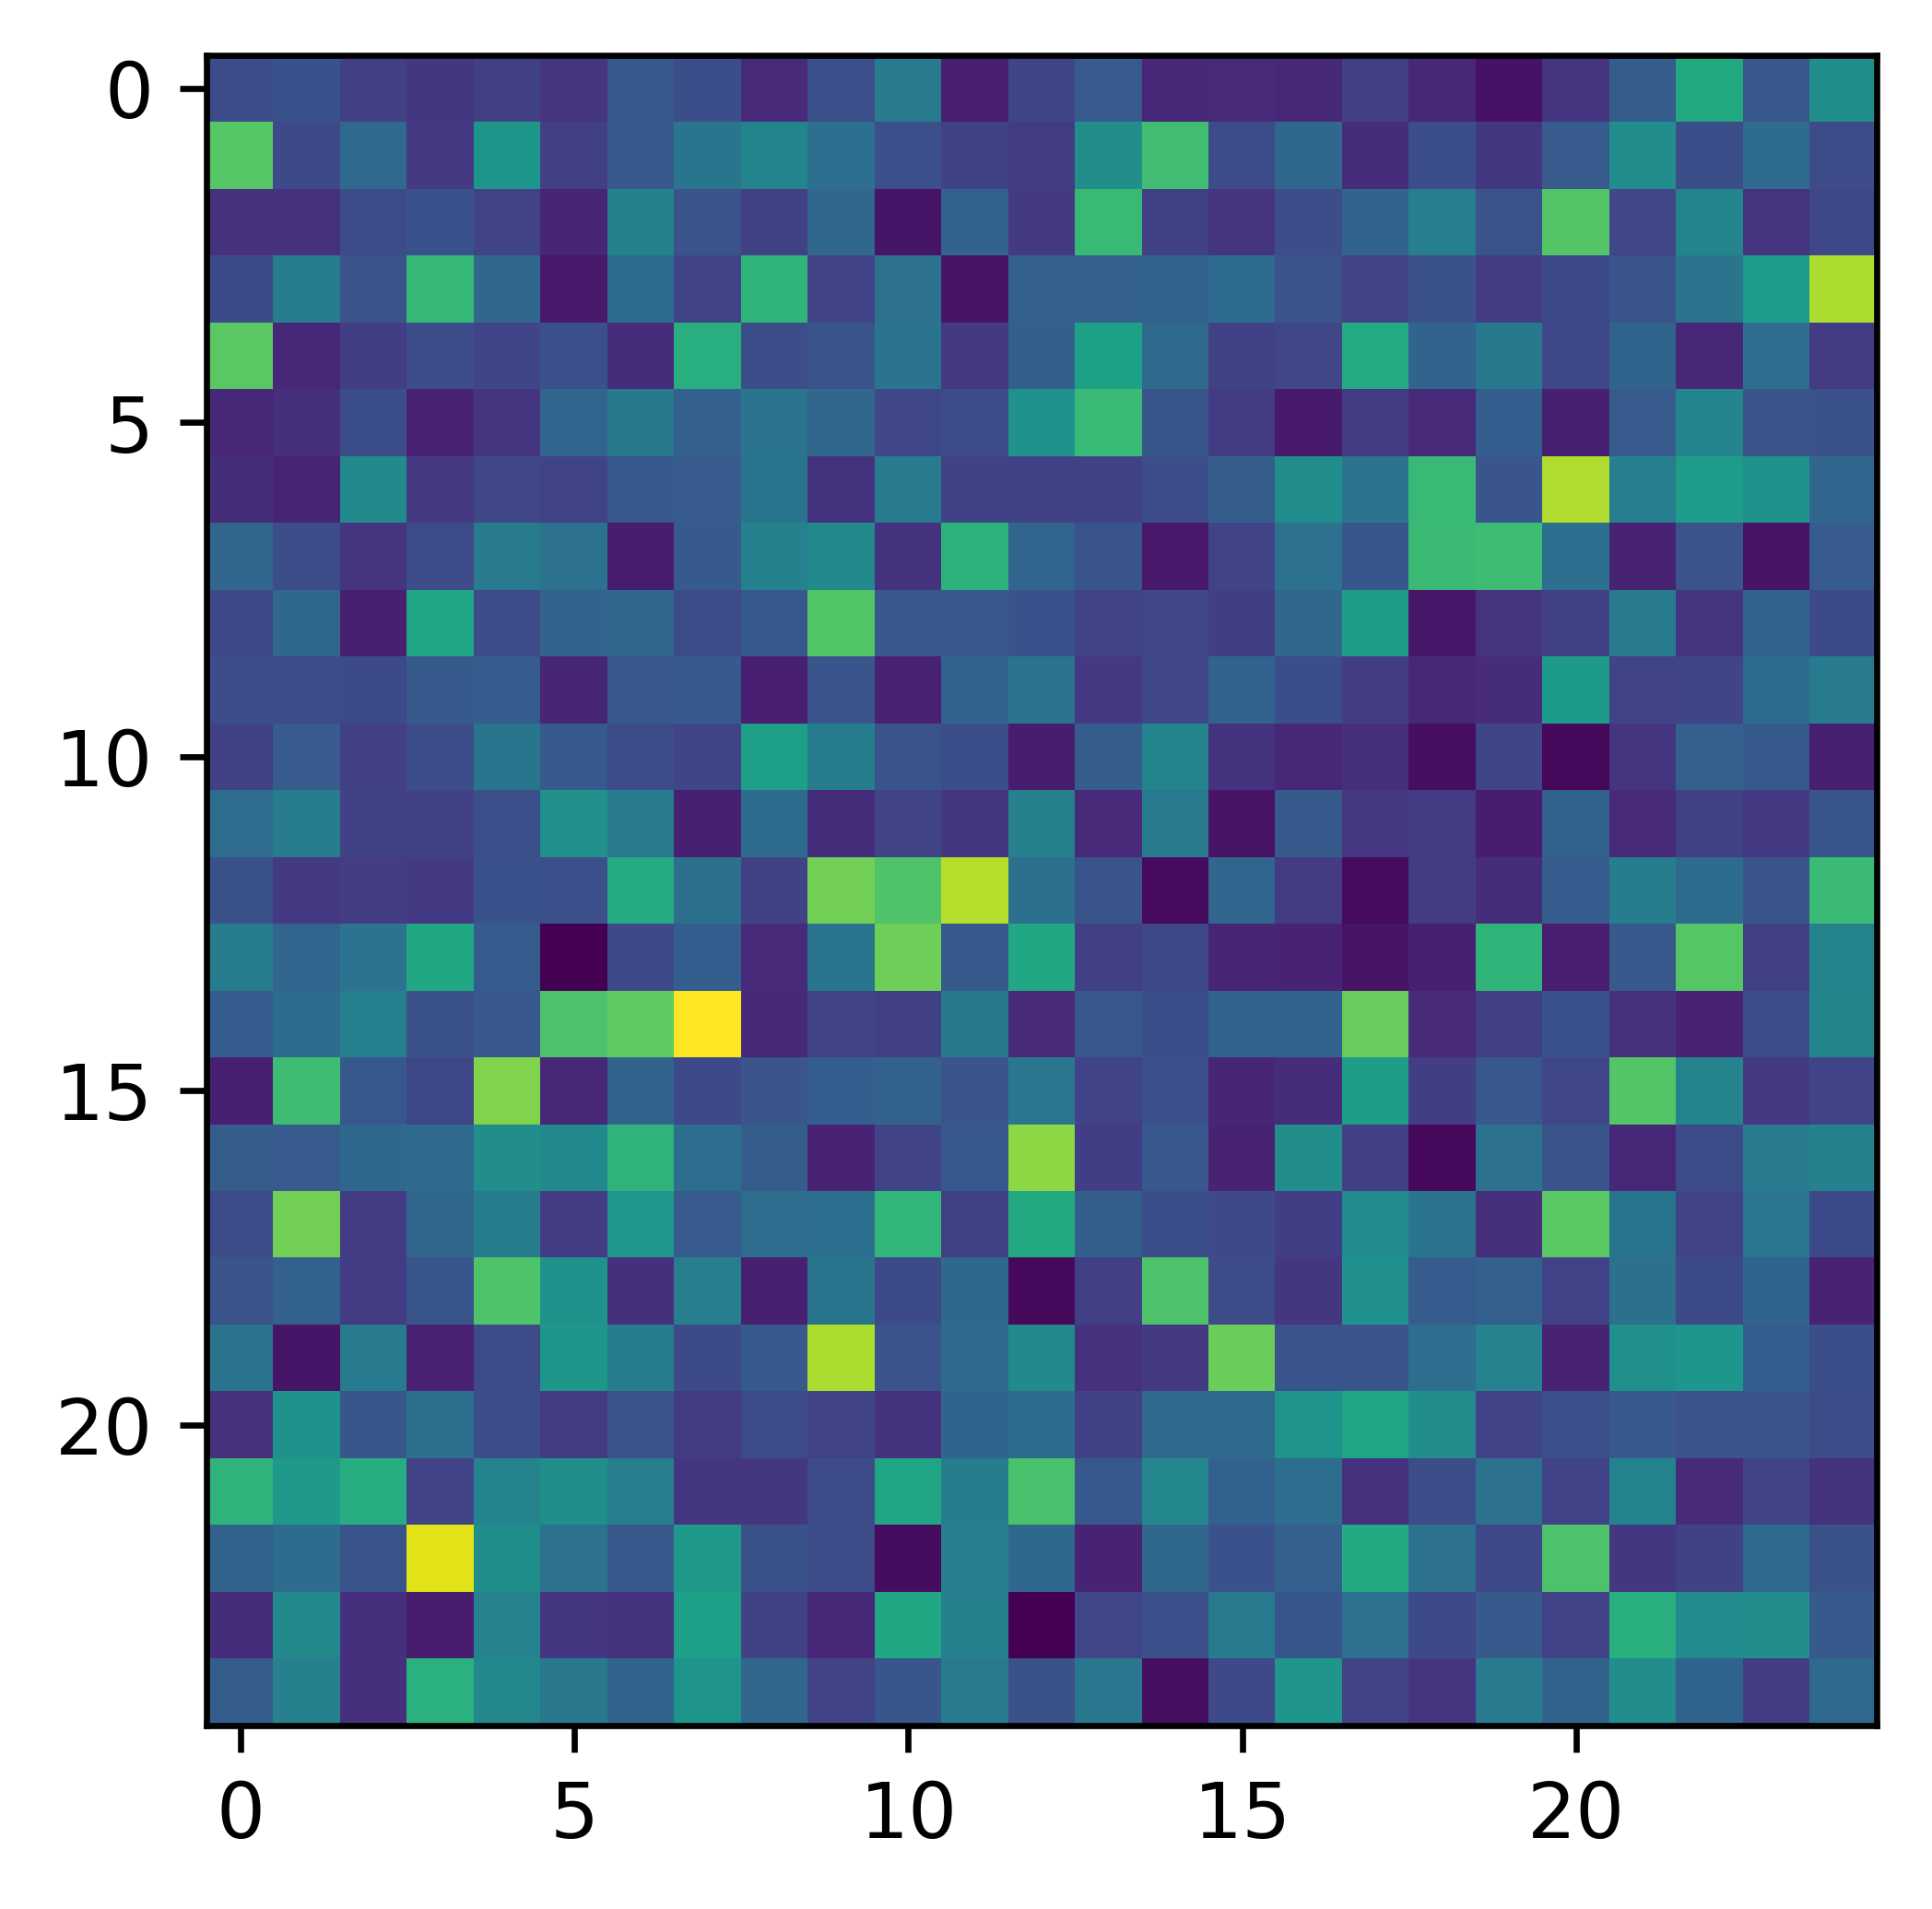
\includegraphics[width=\linewidth]{Graphics/gaussian-2d-experiment-horizontal.png}\par 
    \end{multicols}
\begin{multicols}{2}
    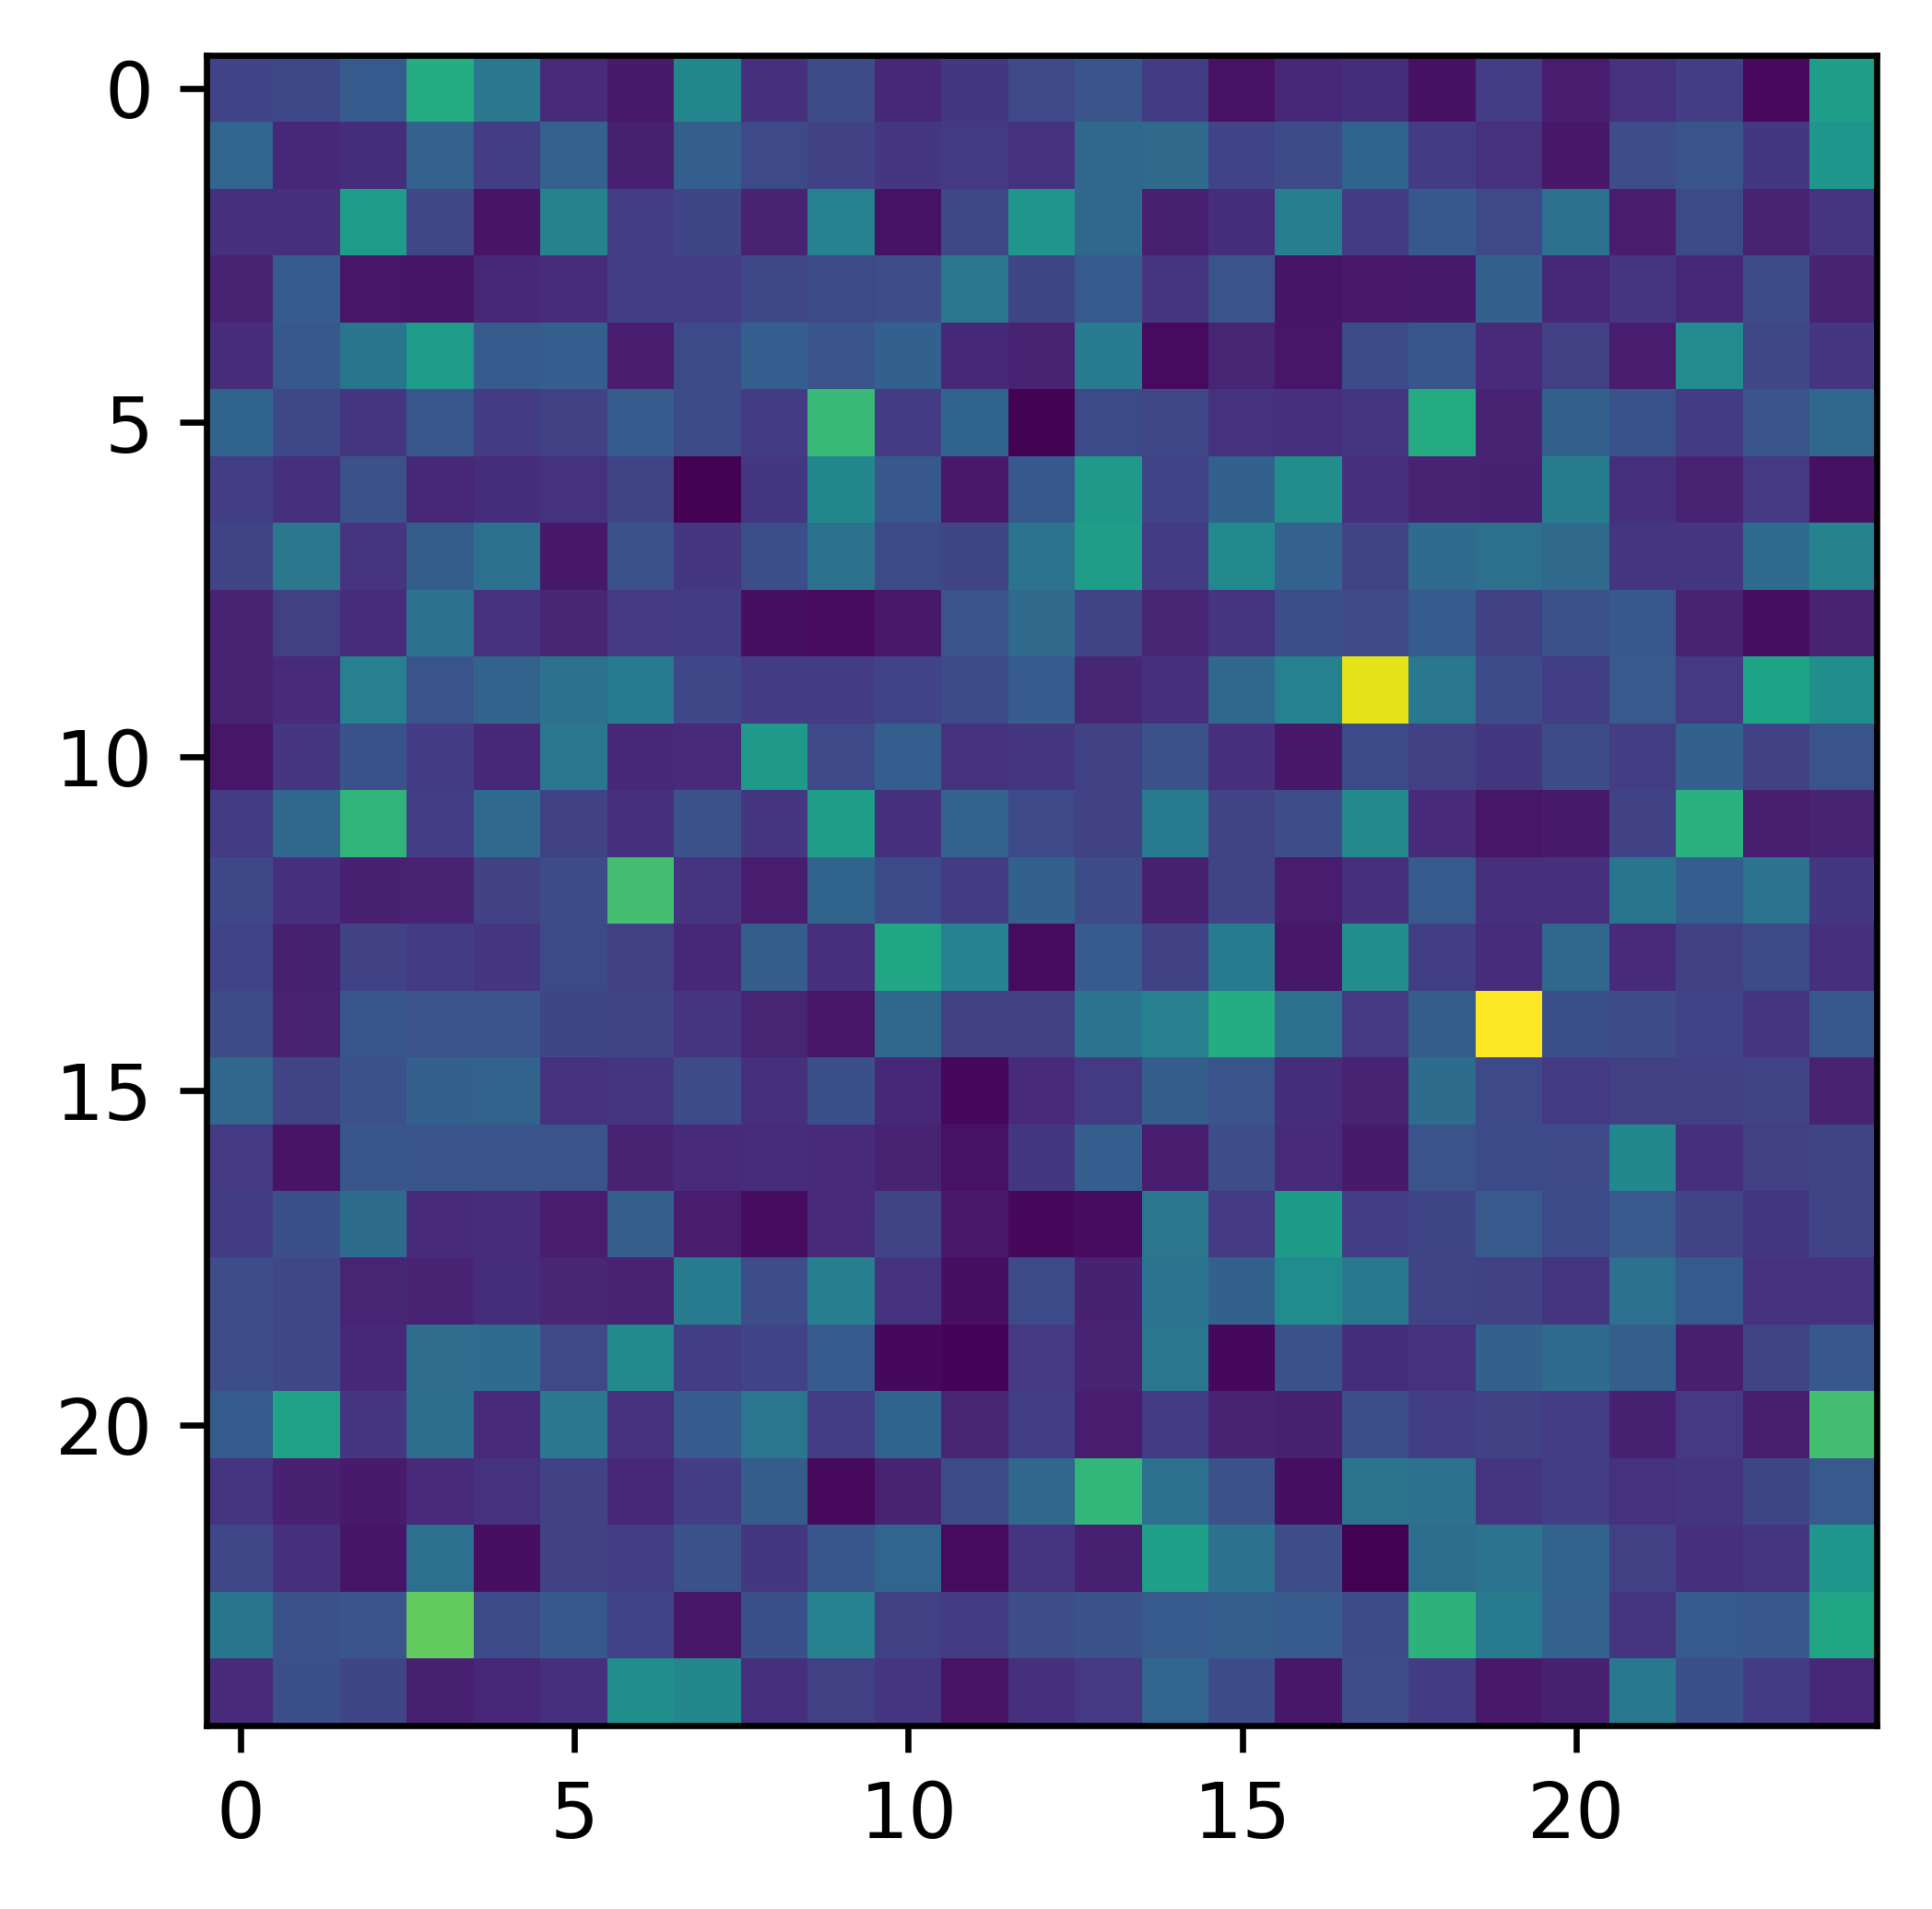
\includegraphics[width=\linewidth]{Graphics/gaussian-2d-experiment-vertical.png}\par
    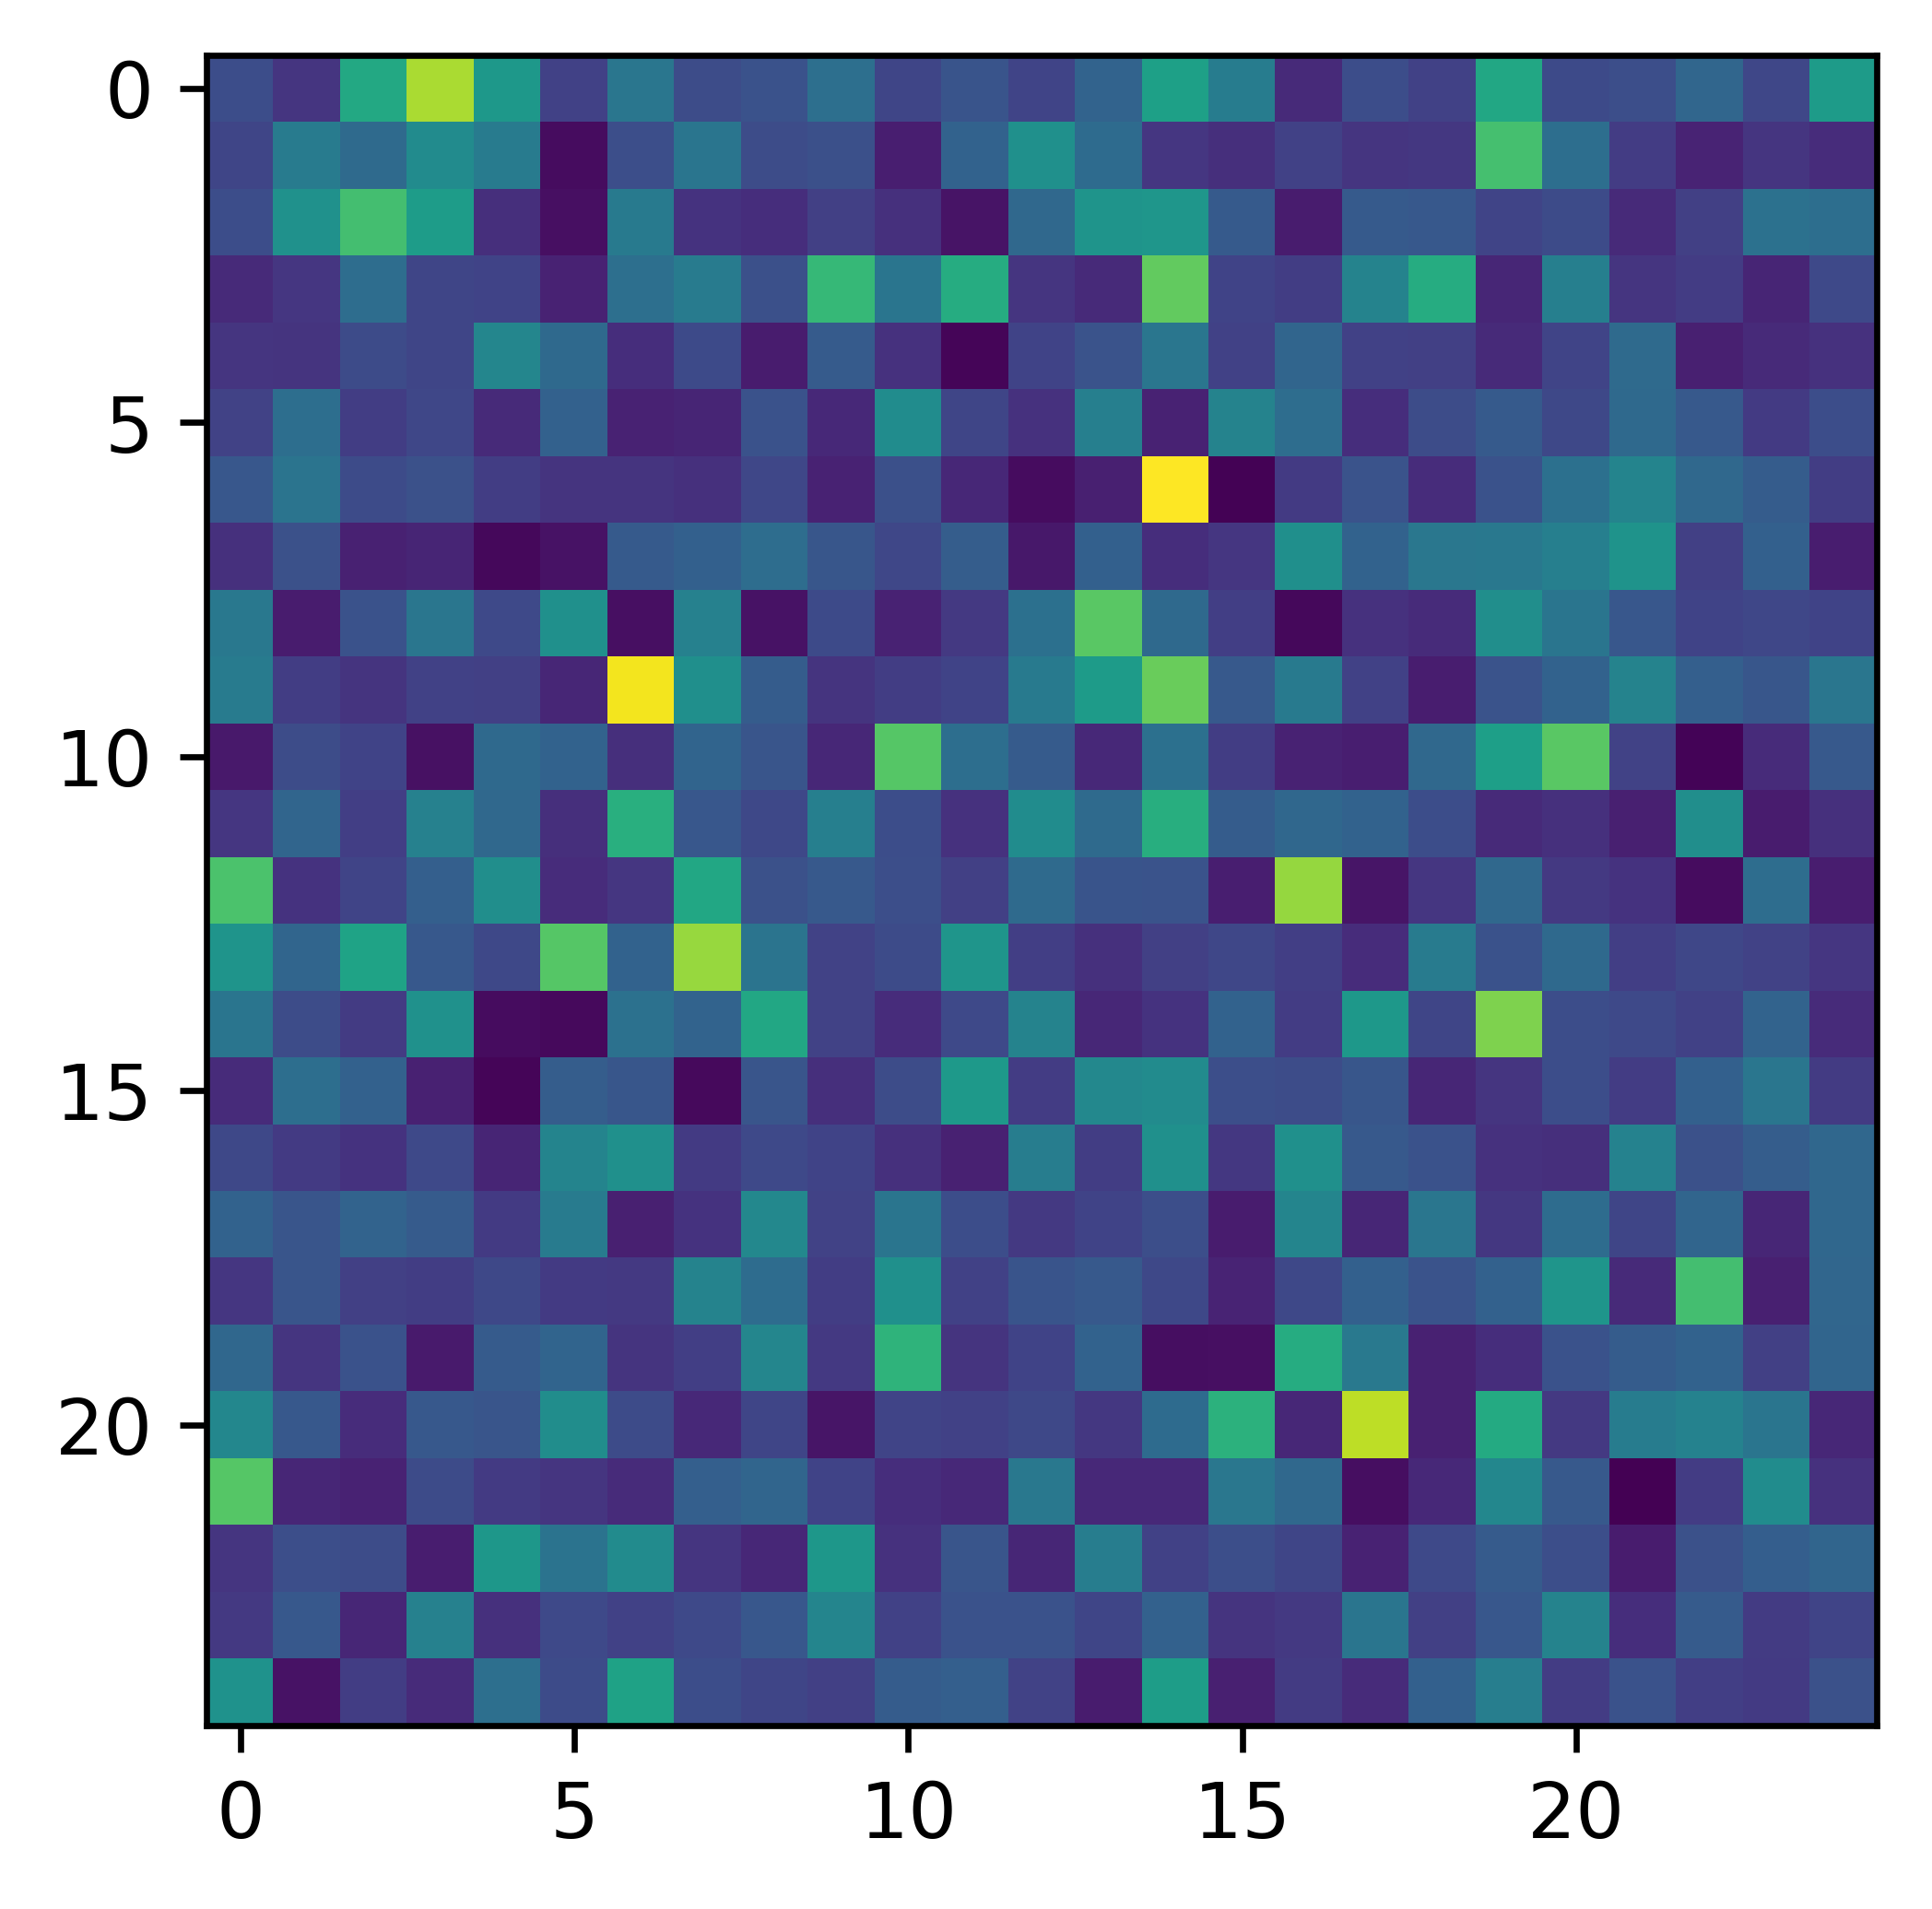
\includegraphics[width=\linewidth]{Graphics/gaussian-2d-experiment-diagonal.png}\par
\end{multicols}
\caption{Resultado de evaluar $S$ sobre cada uno de las componentes de la DST-II usando el primer enfoque} \label{fig:gaussian-example-approach1}
\end{figure*}


El resultado del segundo enfoque se aprecia en la figura \ref{fig:gaussian-example-approach2}.
En esta caso si se puede apreciar claramente en el caso de la DST-II por filas que existe un coeficiente que sobresale
entre los demás. El mismo se encuentra en la posición $(30,16)$ con un valor de $S=0.9797916324922307$.
Esta posición corresponde aproximadamente al punto $30,34$ en la imagen original. Teniendo en cuenta que 
sección horizontal del patrón tomado esta comprendida en el intervalo $[30,25:40]$ el resultado es bastante certero.

En el caso de la sección vertical, no se tuvo tanto éxito. No existe gran constraste entre un posición con el resto. Esto
se debe a que el error de las condiciones de matching es mucho mayor para la shapelet de la sección vertical que para las
de las sección horizontal.

\begin{figure}
	\centering
	\subfigure[Por filas]{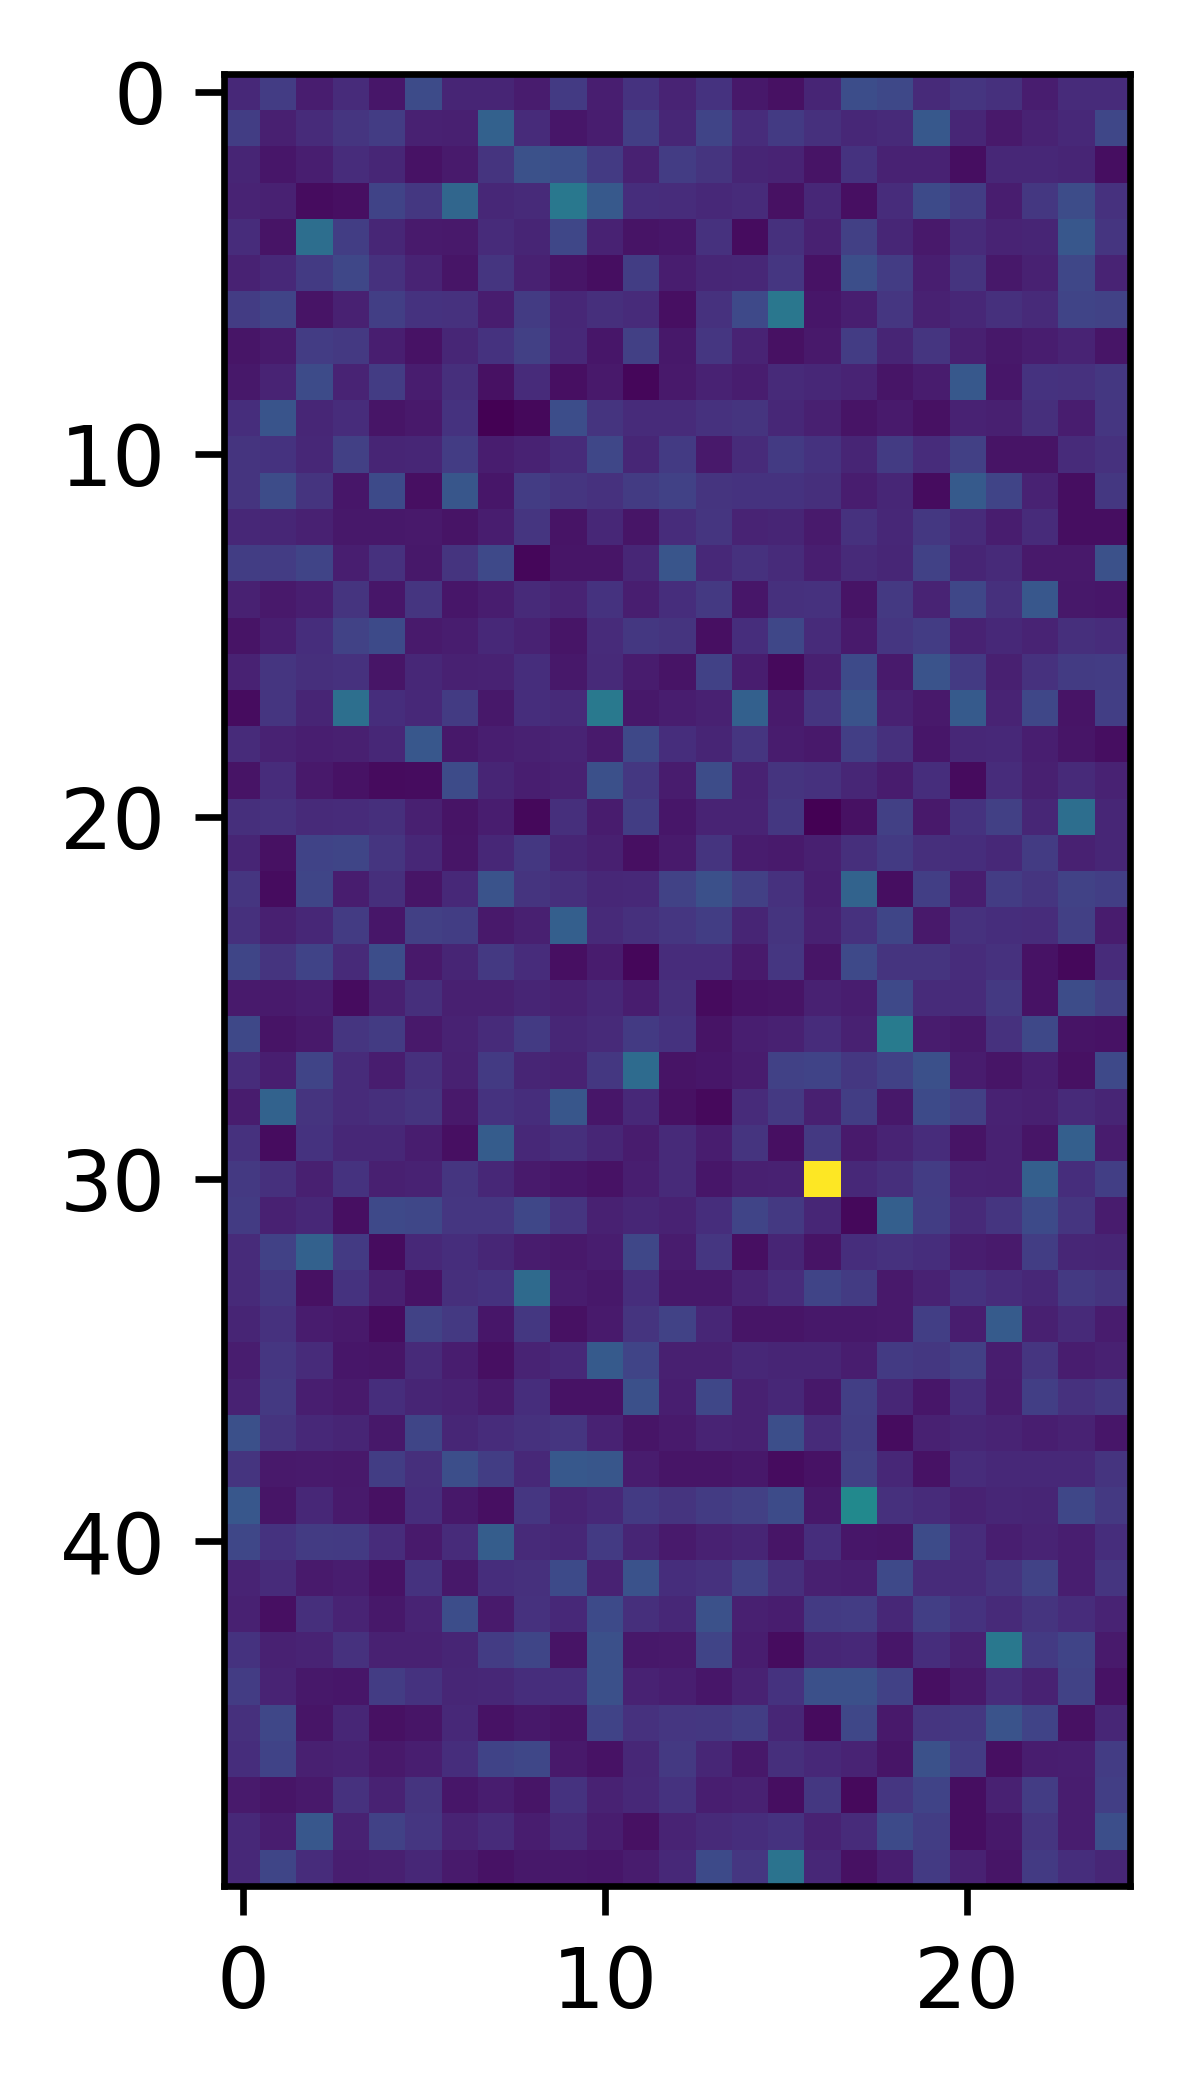
\includegraphics{Graphics/gaussian-2d-experiment2-row.png}}
	\subfigure[Por columnas]{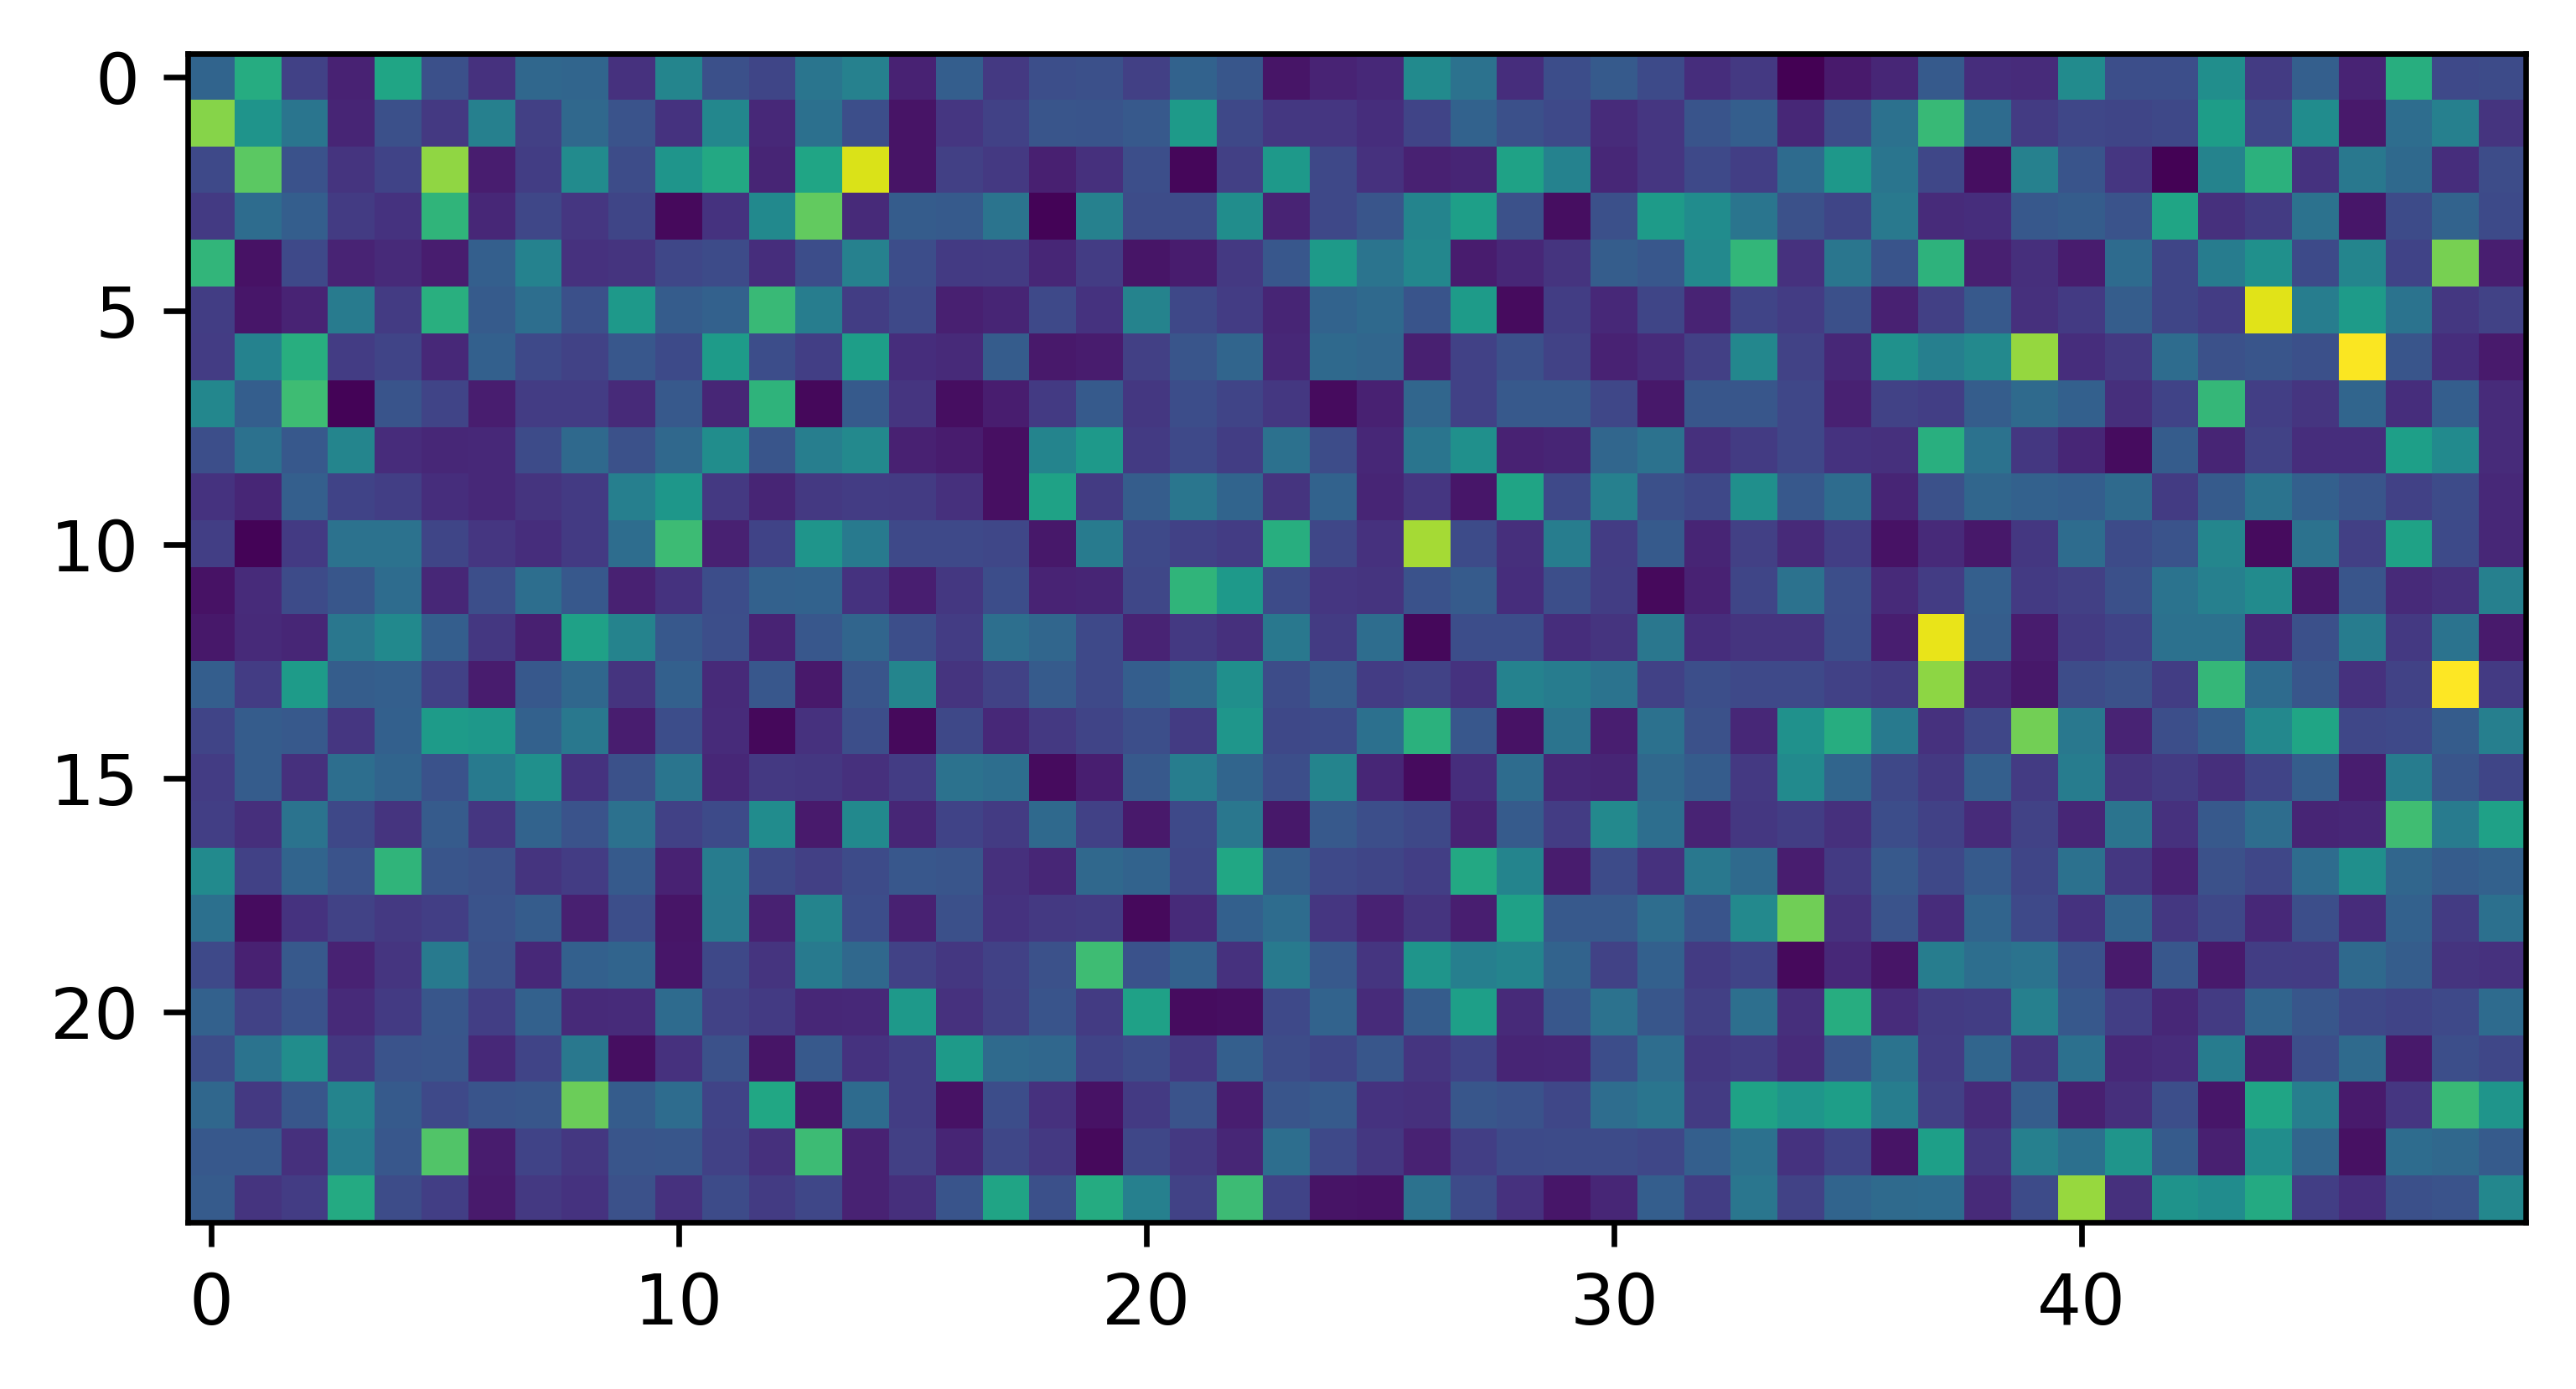
\includegraphics{Graphics/gaussian-2d-experiment2-col.png}}
	\caption{Resultado de evaluar $S$ sobre cada cada una de las \textit{second-rated} de la DST-II usando el segundo enfoque.} \label{fig:gaussian-example-approach2}
\end{figure}
%-0.00781404414483181 col error matching
%0.0118491040034377
%-2.61711684291969e-18 row error matchine
%-8.05175395622083e-18

En el caso del tercer enfoque, se toma la región comprendida entre los píxeles $[25:40,25:40]$. Los resultados se muestran
en \ref{fig:gaussian-example-approach3}. En este caso se logra obtener toda una región con mayor contrate que corresponde aproximadamente
a las posiciones donde se encuentra el patrón. Sin embargo, muchos de estos valores realmente no sobrepasan el umbral $0.7$,
por el hecho de una parte de los filtros calculados tienen errores altos en las condiciones de matching, por lo que
no detectan bien su sección del patrón correspondiente y al promediar los resultados introducen ruido en el resultado final.
Esto limita considerablemente la capacidad de detectar una región entera usando este enfoque. Otra desventaja es el costo
computacional. Resolver varios sistemas de ecuaciones no lineales puede tomar bastante tiempo.

\begin{figure}
	\centering
	\subfigure[Por filas]{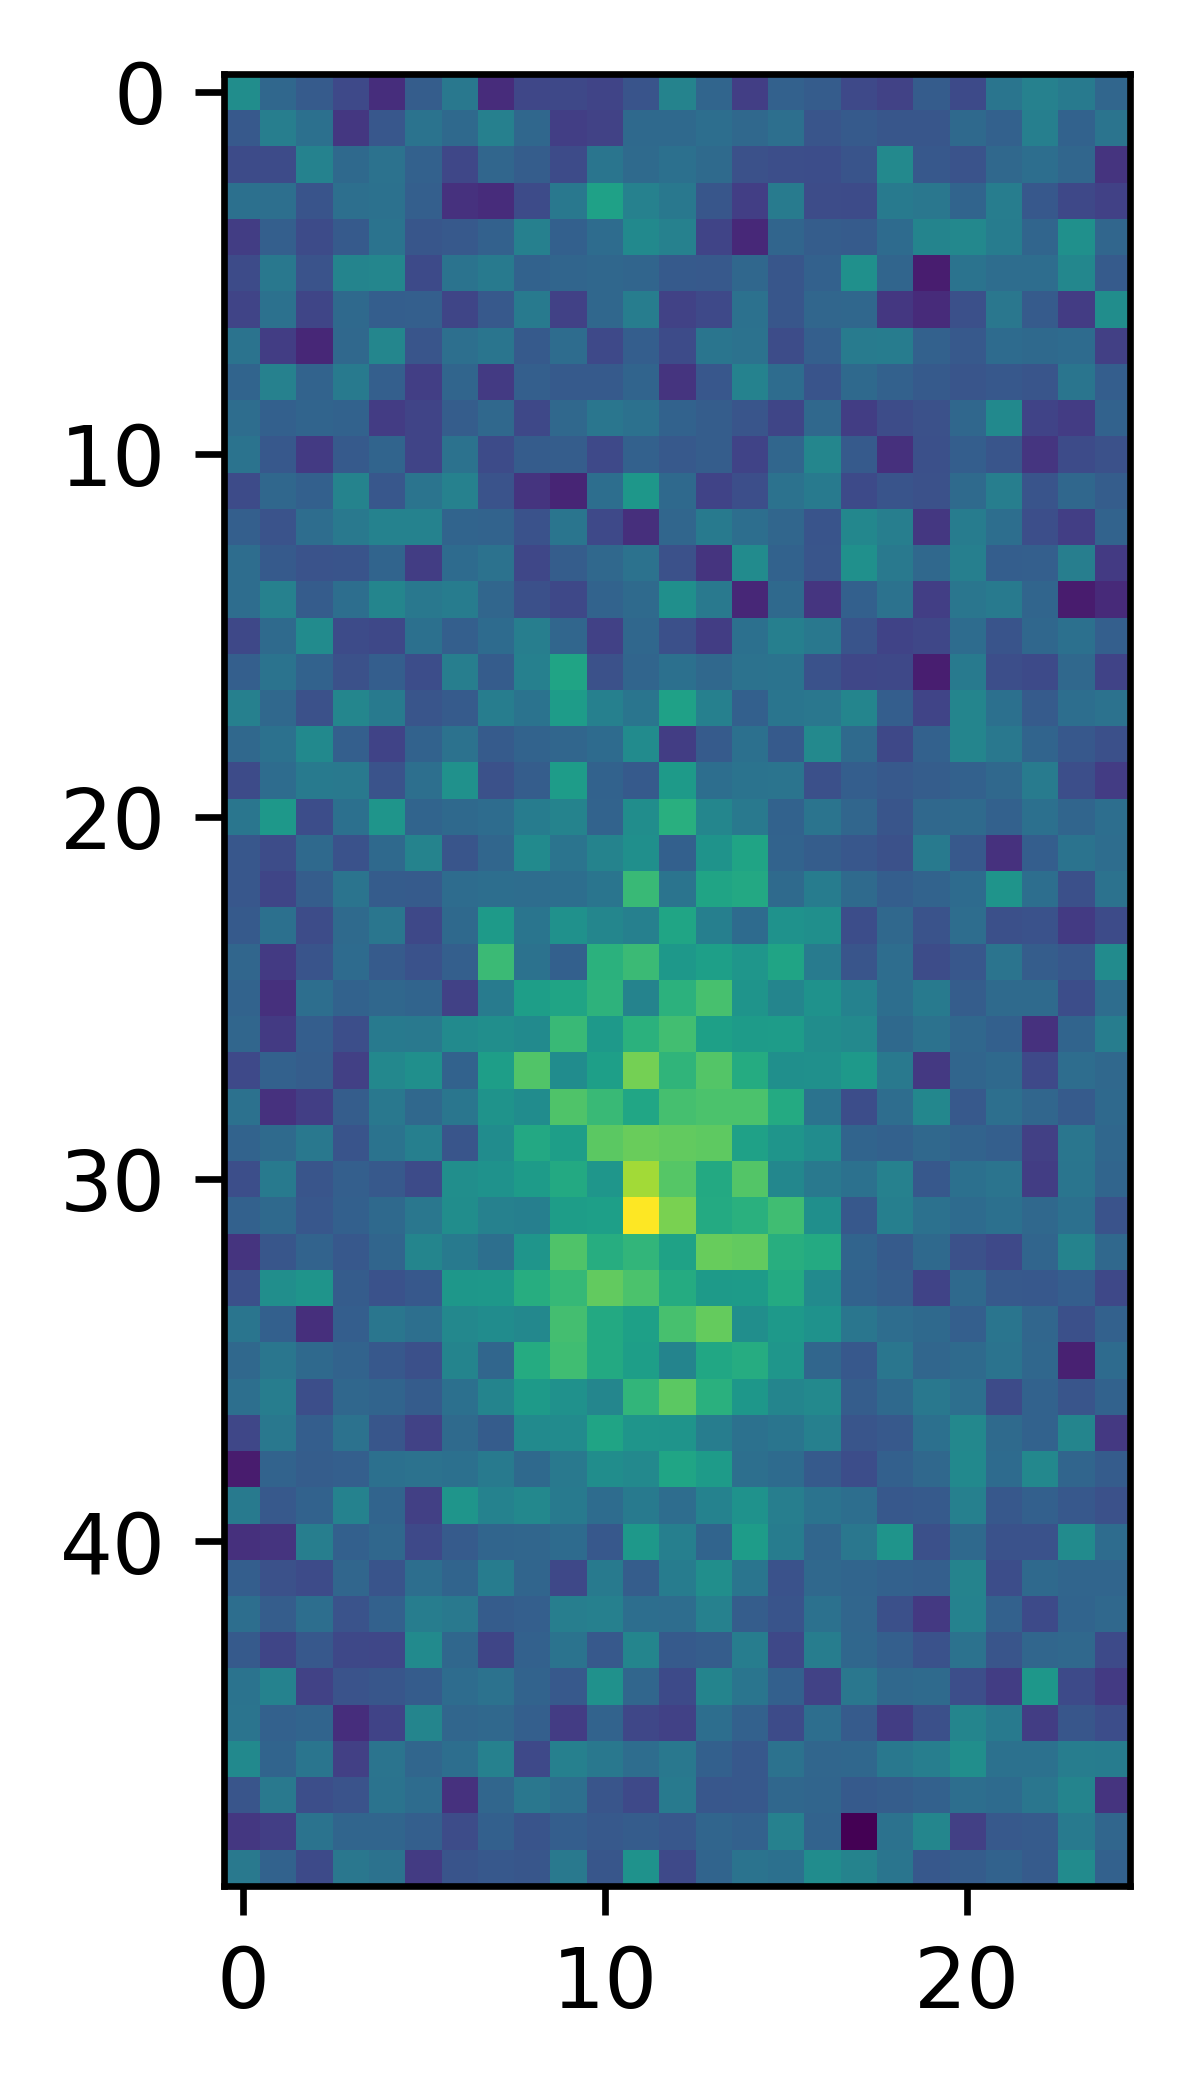
\includegraphics{Graphics/gaussian-2d-experiment3-row.png}}
	\subfigure[Por columnas]{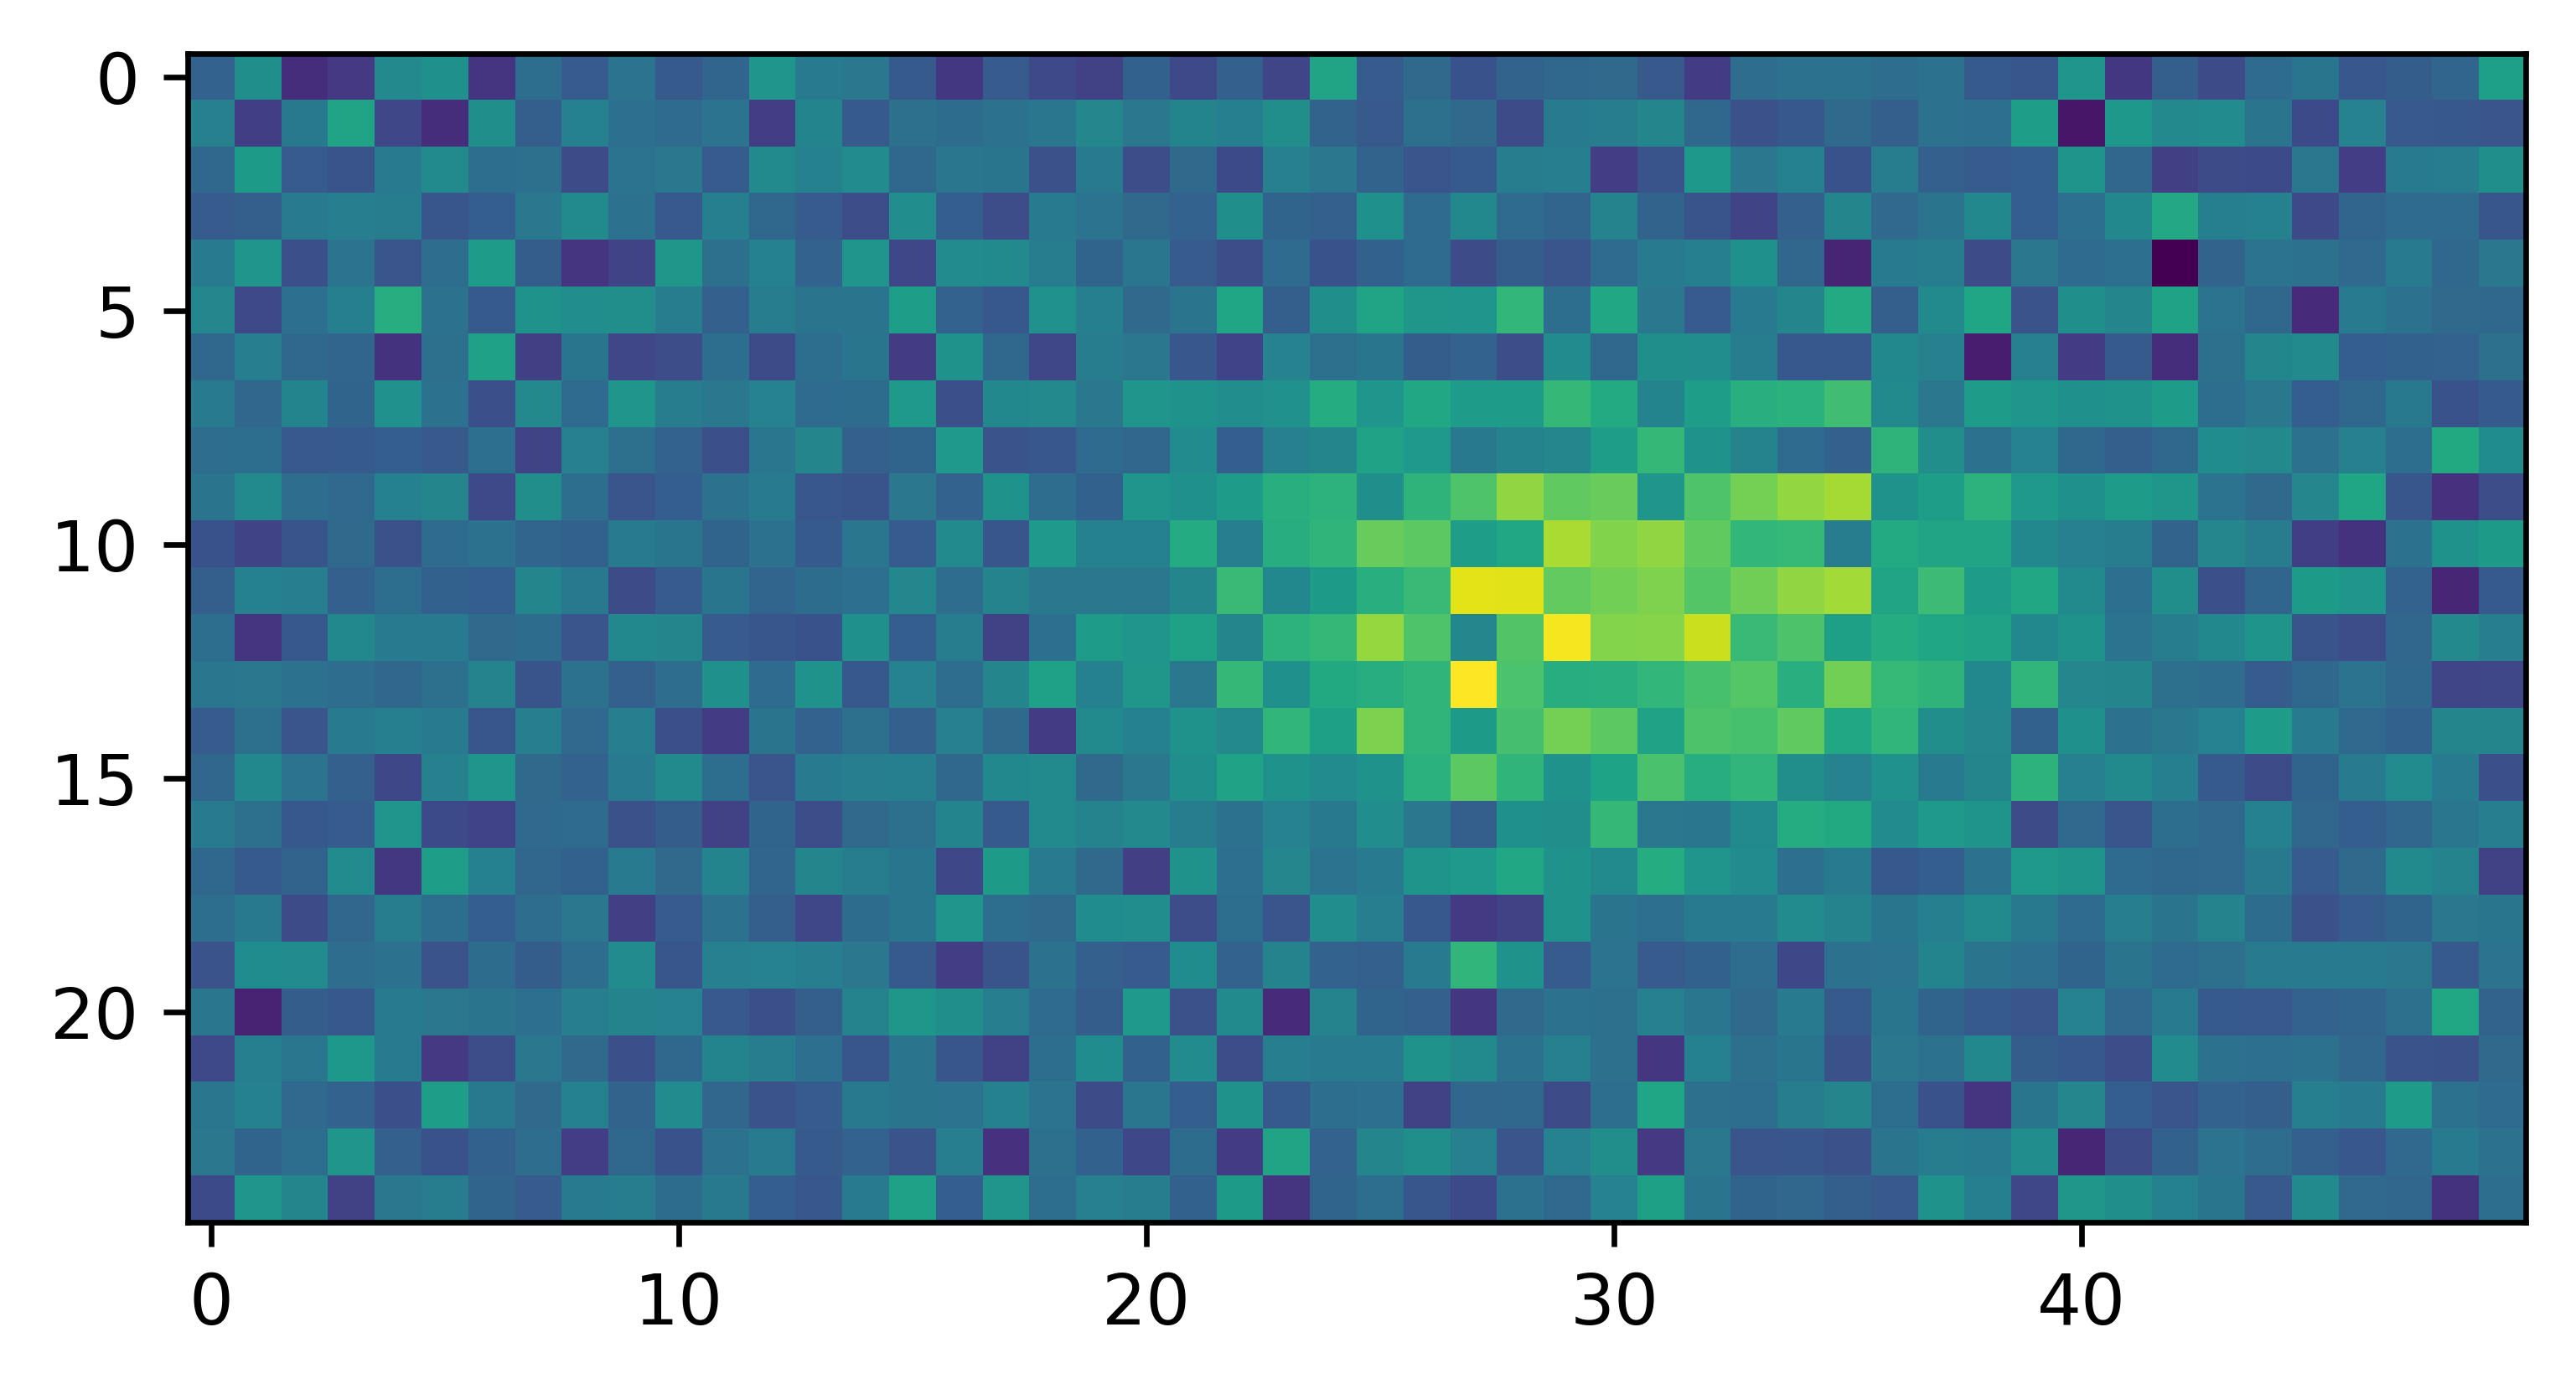
\includegraphics{Graphics/gaussian-2d-experiment3-col.png}}
	\caption{Resultado de evaluar $S$ sobre cada cada una de las \textit{second-rated} de la DST-II usando el tercer enfoque.} \label{fig:gaussian-example-approach3}
\end{figure}

\section{Applicación en la detección de masas en mamografías}

Para evaluar la capacidad del algoritmo de la DST-II y las propuestas de extensión al caso bidimensional en
la detección de masas de mamografías se usó la base de datos \textbf{INBreast} \cite{Moreira2012}. La misma 
contiene un totla de 115 casos ( 410 imágenes ), todas con anotaciones sobre distintos tipos de lesiones. 
En este caso son de interés las de tipo masas, específicamente las que presentan isometría.

Las imágenes poseen una resolución de $3328\times 4084$ or $2560\times 3328$ y están guardadas en formato
DICOM. Para su lectura se usó la biblioteca Pydicom.

Dado que las imágenes tienen una resolución bastante grande se realiza un pre-procesamiento antes de ser pasadas al
algoritmo. Como primer paso se realiza un \textit{rescaling} de las imágenes. Para esto se usa la función de scikit-image
\textbf{skimage.transform.rescale} con un factor de $\frac{1}{8}$ \cite{skimage-transform}. Luego de este \textit{rescaling}
se realiza un suavizado a la imagen y un \textit{sharpening}. El primer se realiza con un filtro guassiano
para eliminar la existencia de ruido en la mamografía. Para el segundo se usa un filtro laplaciano con el objetivo
de detectar mejor los bordes. Ambos resultados se fusionan y es sobre esa imagen sobre la que se utiliza el algoritmo.

A continuación se muestra un ejemplo de los experimentos realizados.

\subsection{Ejemplos de los experimentos y análisis de los resultados}

El ejemplo tomado se muestra en la figura \ref{fig:example-mm}. La imagen muestra los resultados de cada etapa 
del preprocesamiento: \textit{rescaling}, filtro gaussiano, filtro laplaciano y por último fusión de los
resultados de ambos filtros.

\begin{figure*}
\begin{multicols}{2}
    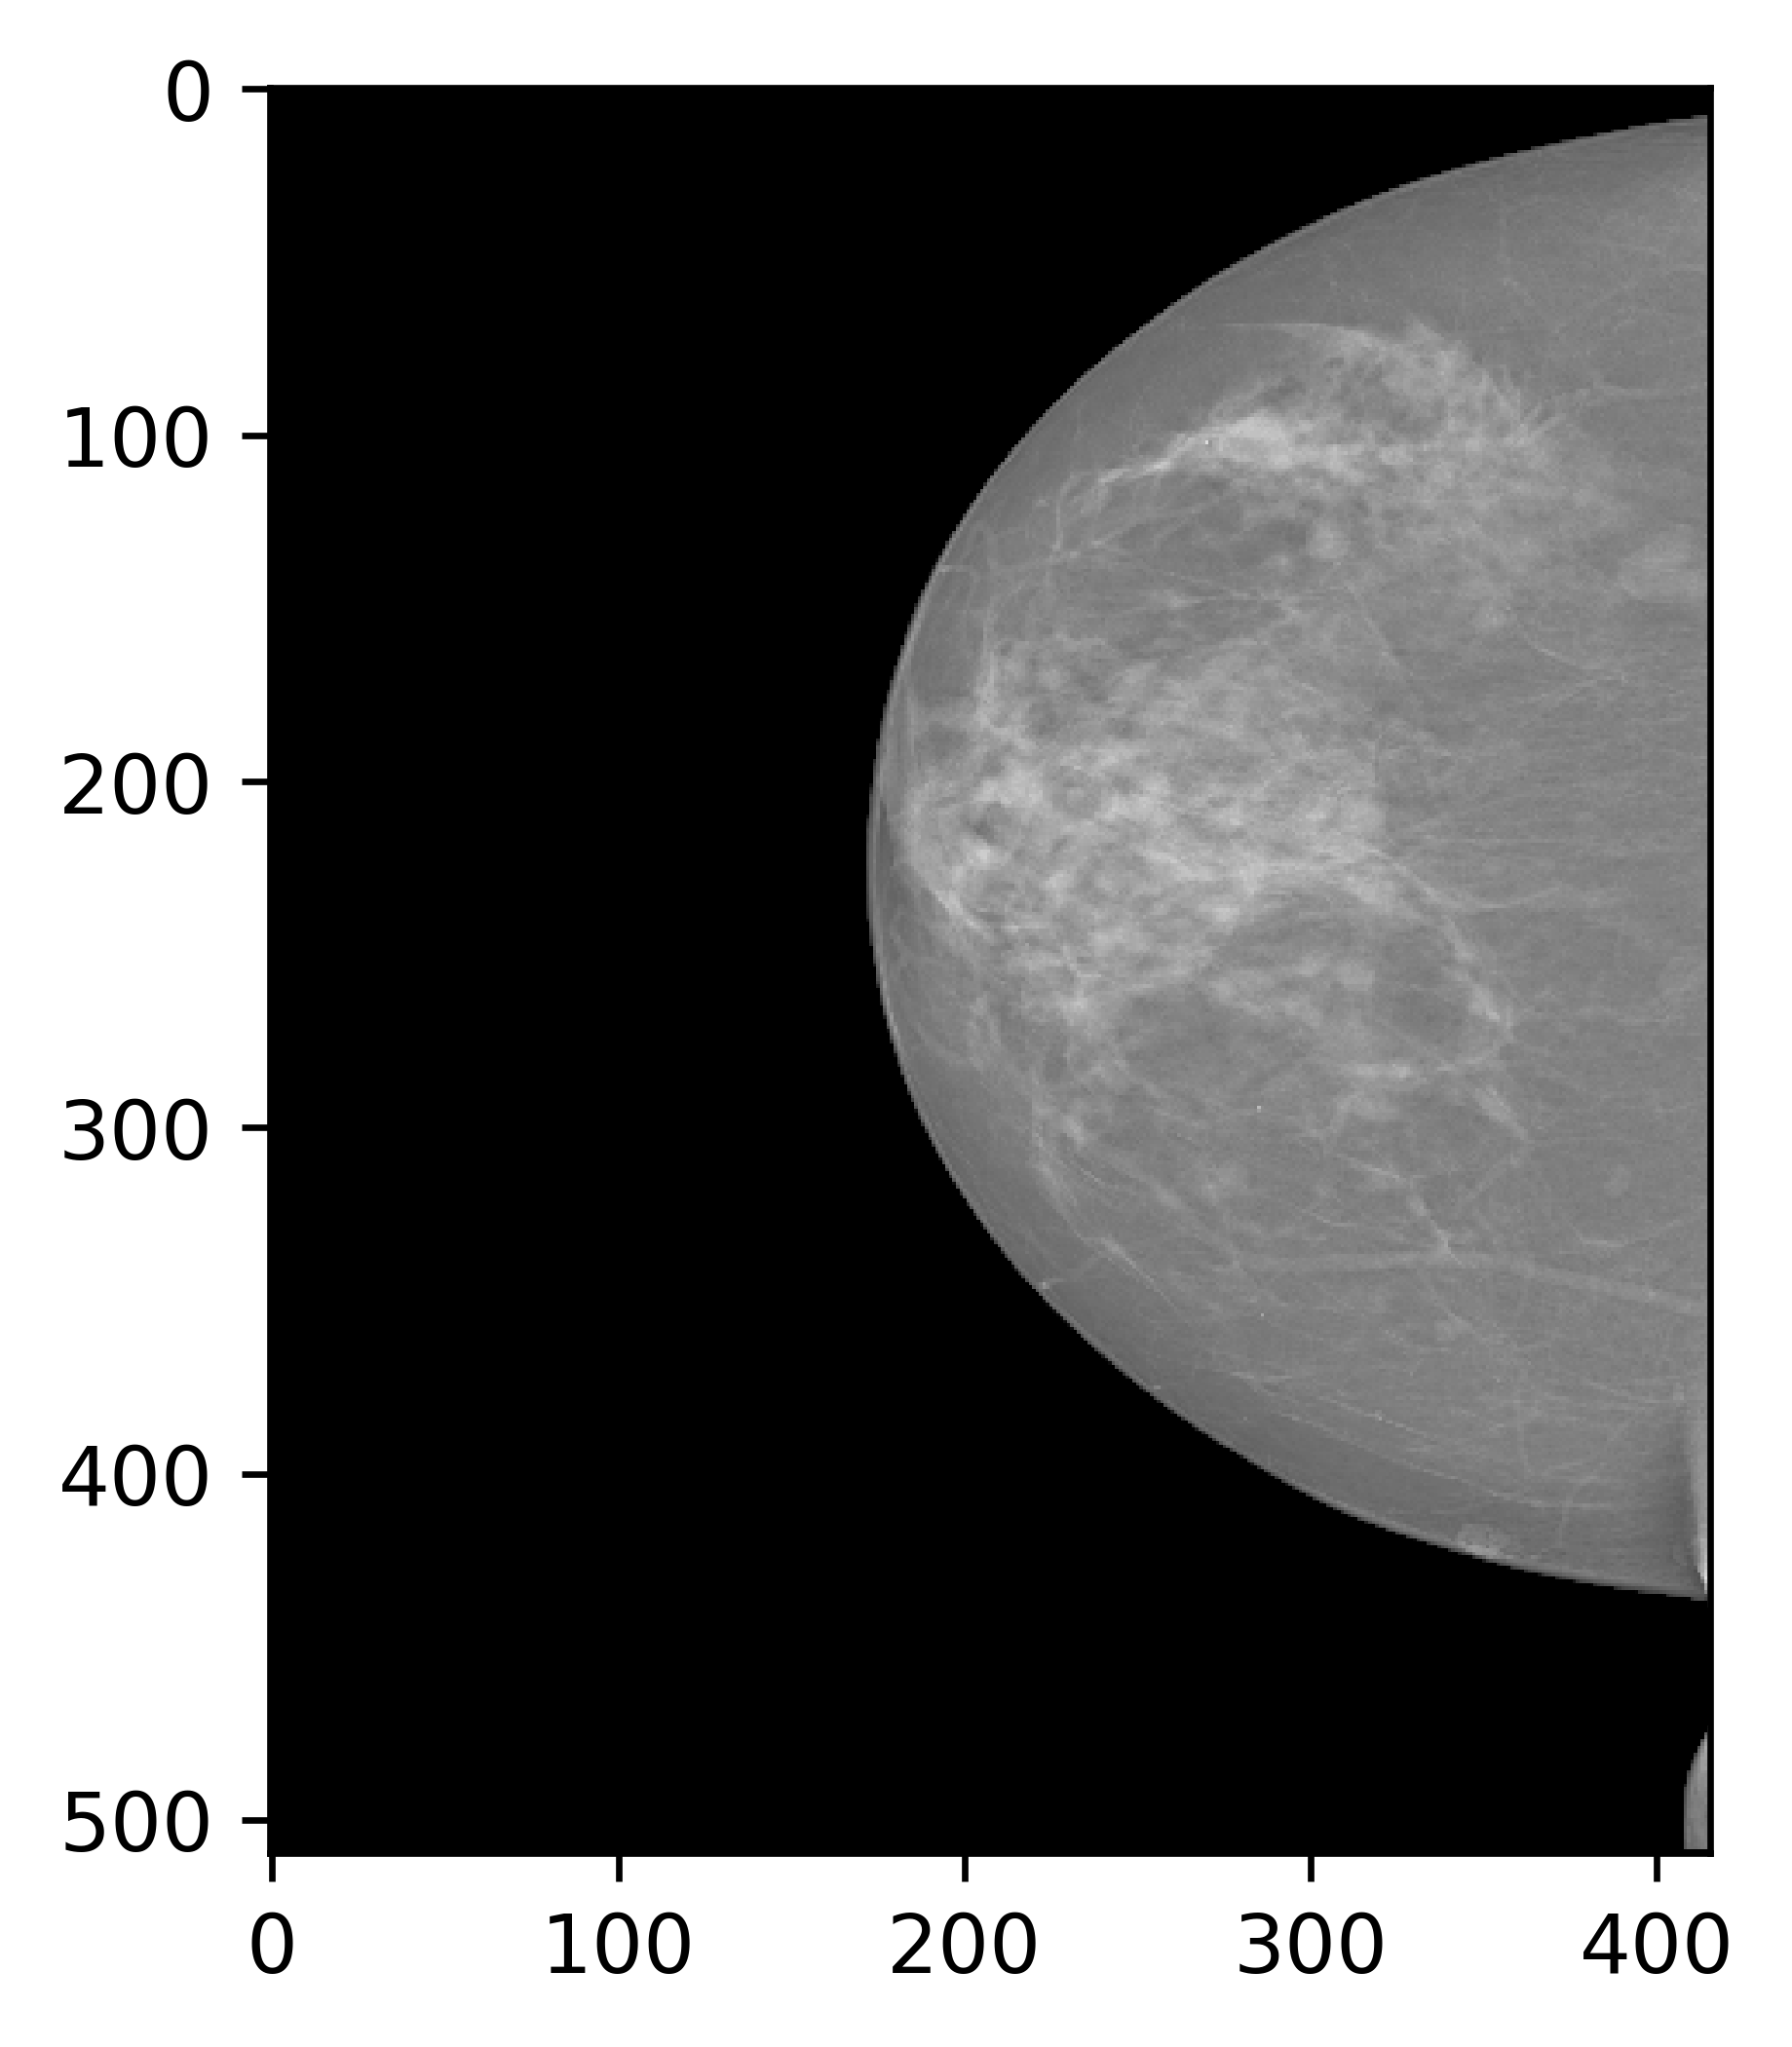
\includegraphics[width=\linewidth]{Graphics/mm-rescaled.png}\par 
    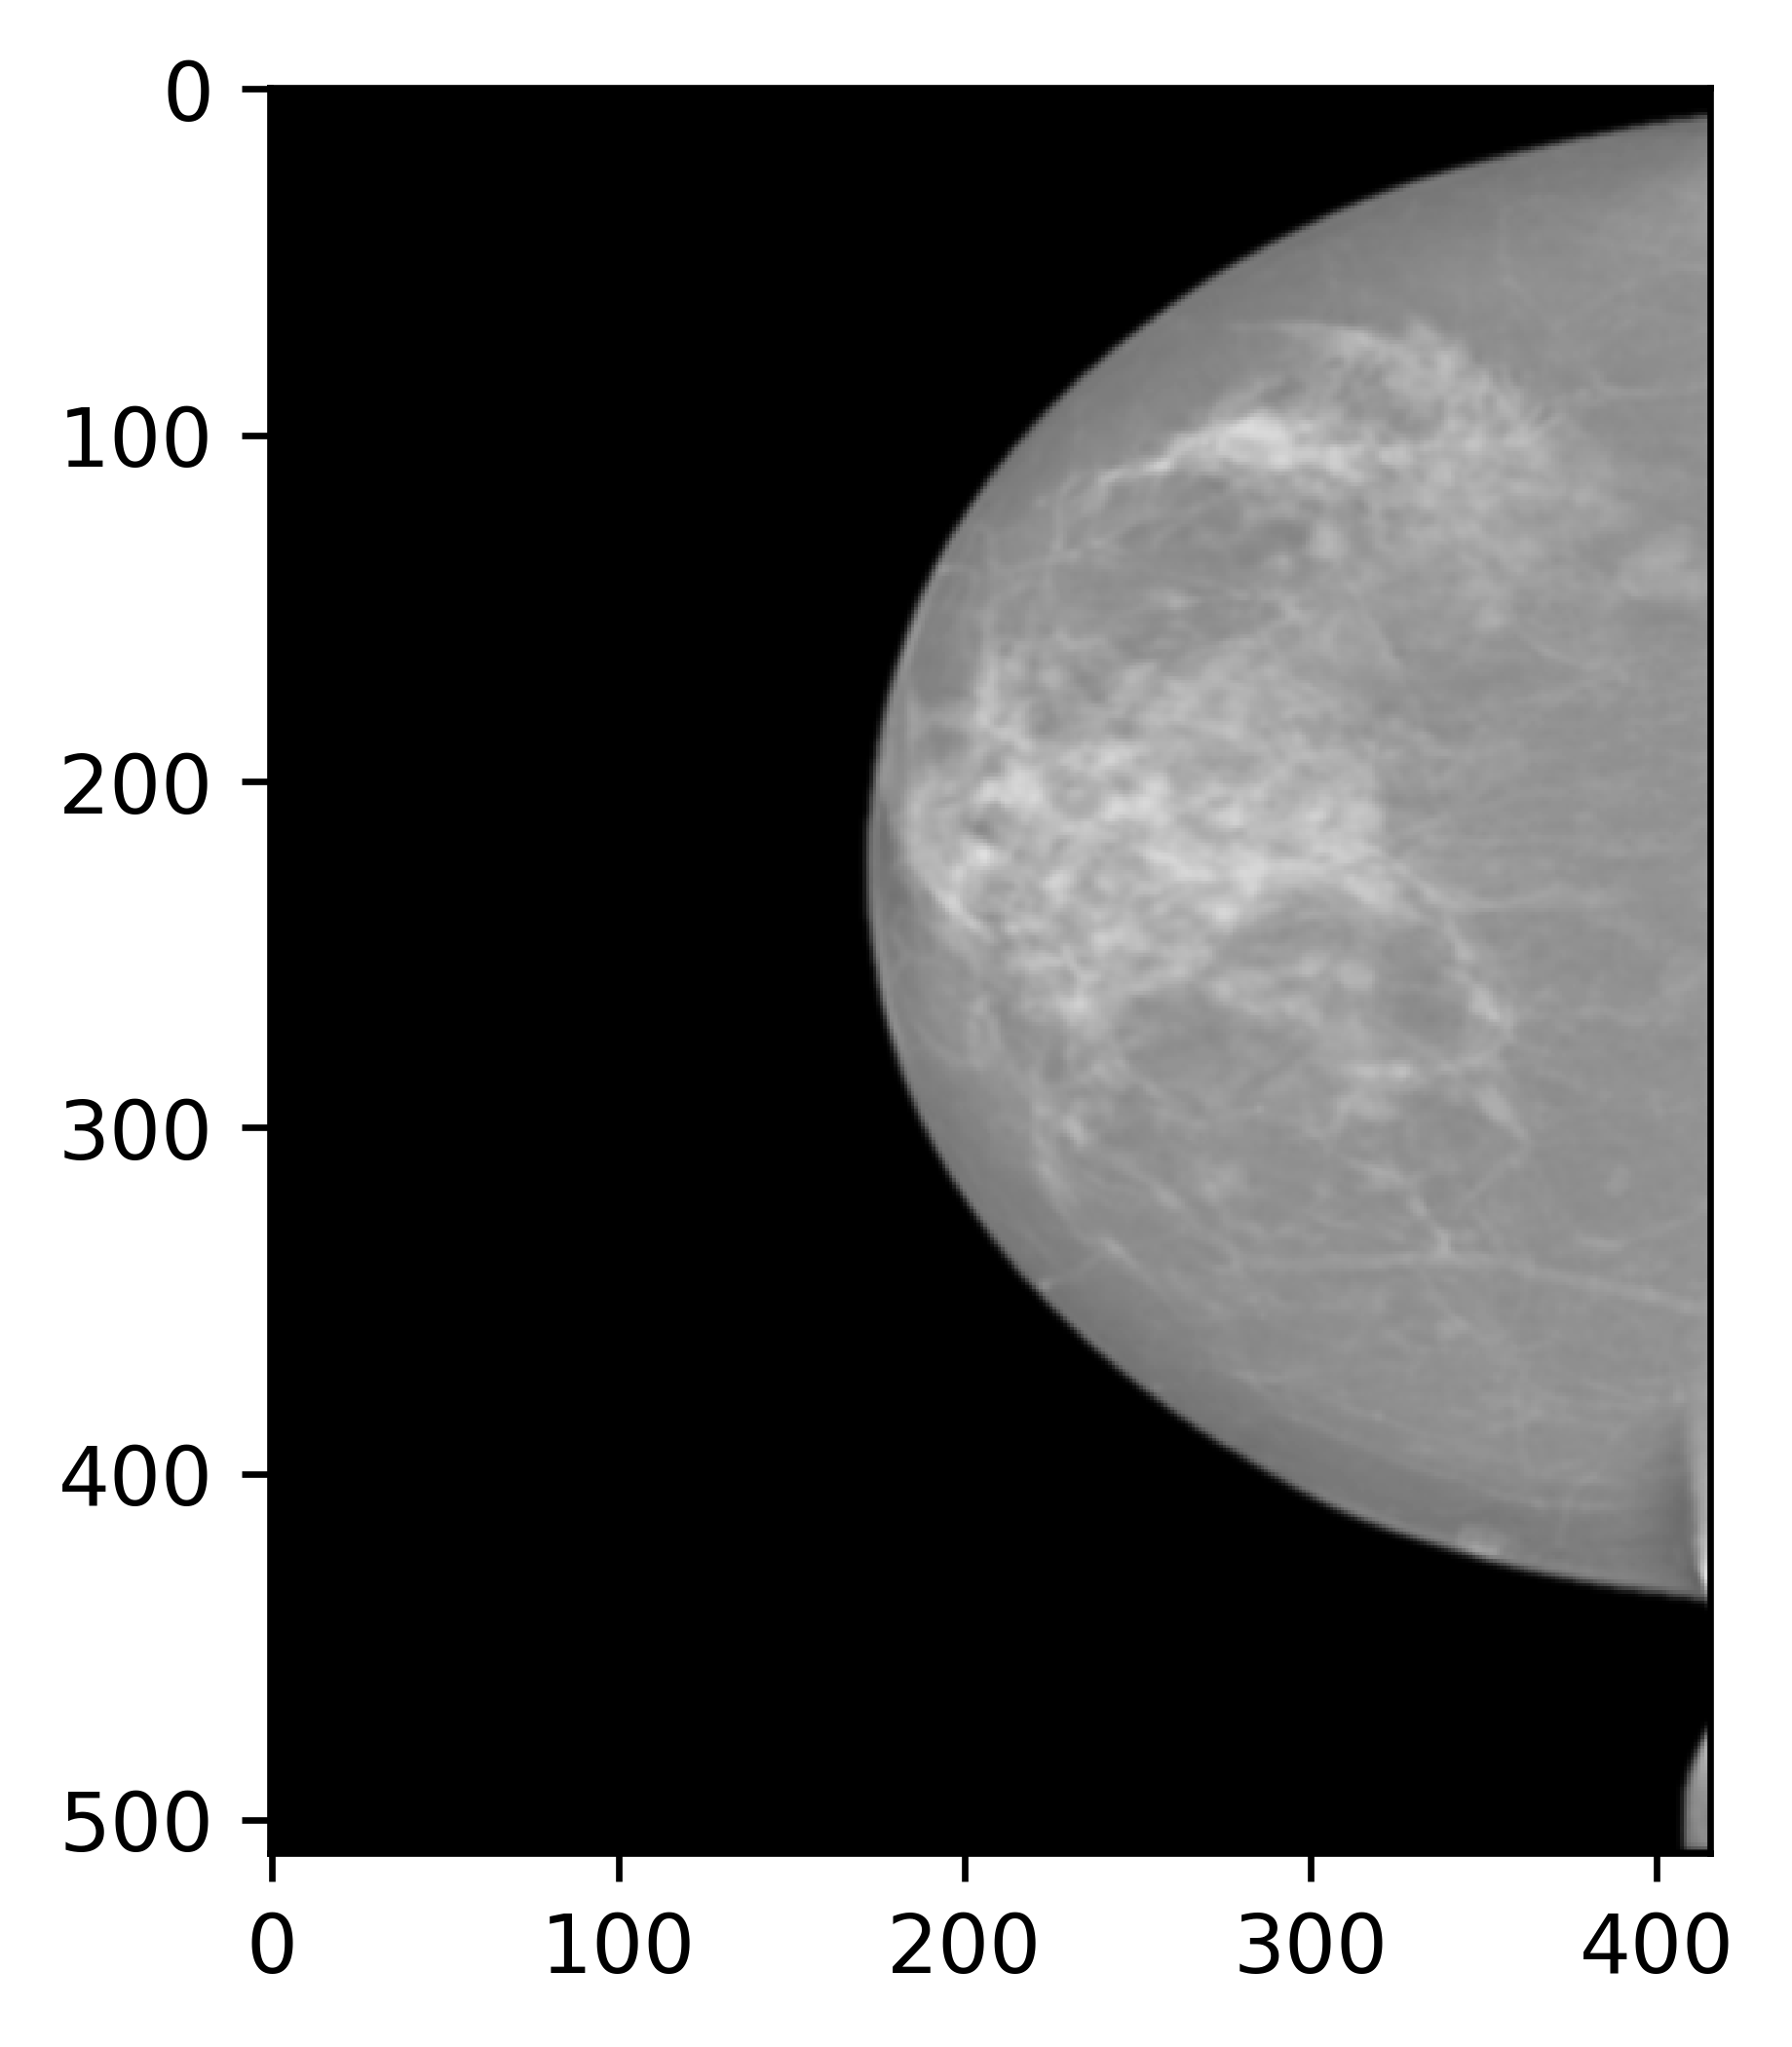
\includegraphics[width=\linewidth]{Graphics/mm-smooth.png}\par 
    \end{multicols}
\begin{multicols}{2}
    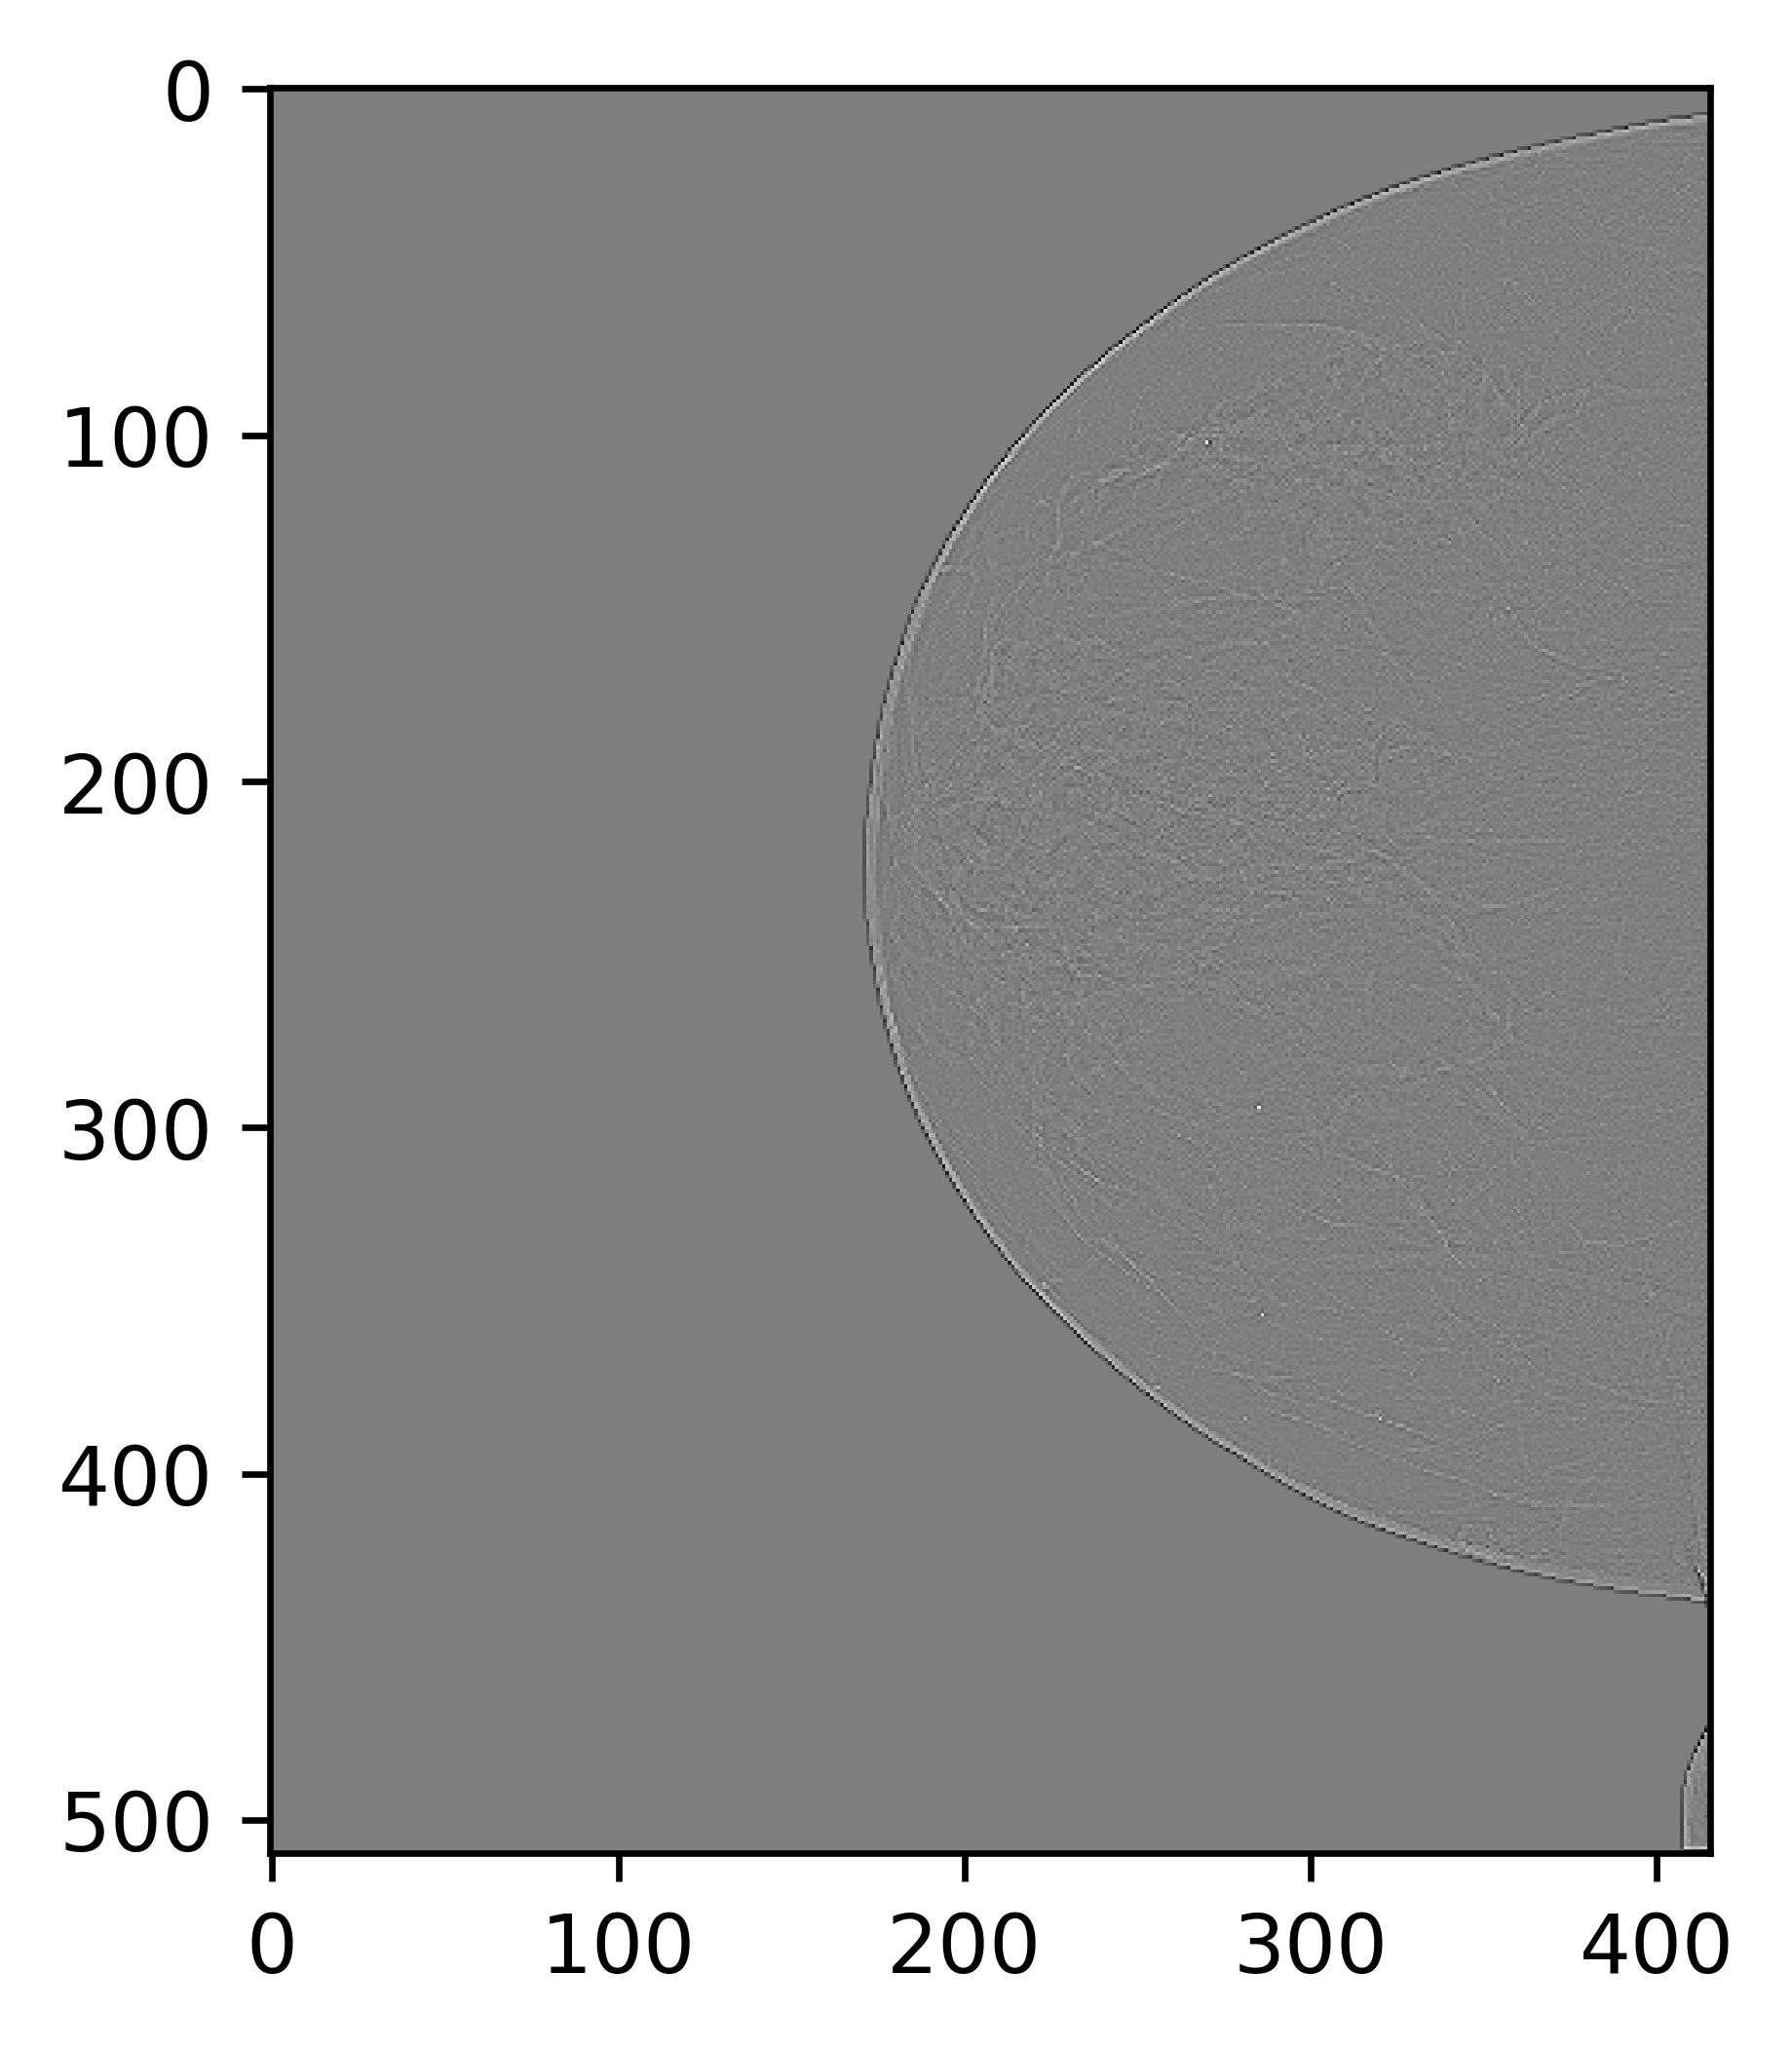
\includegraphics[width=\linewidth]{Graphics/mm-sharp.png}\par
    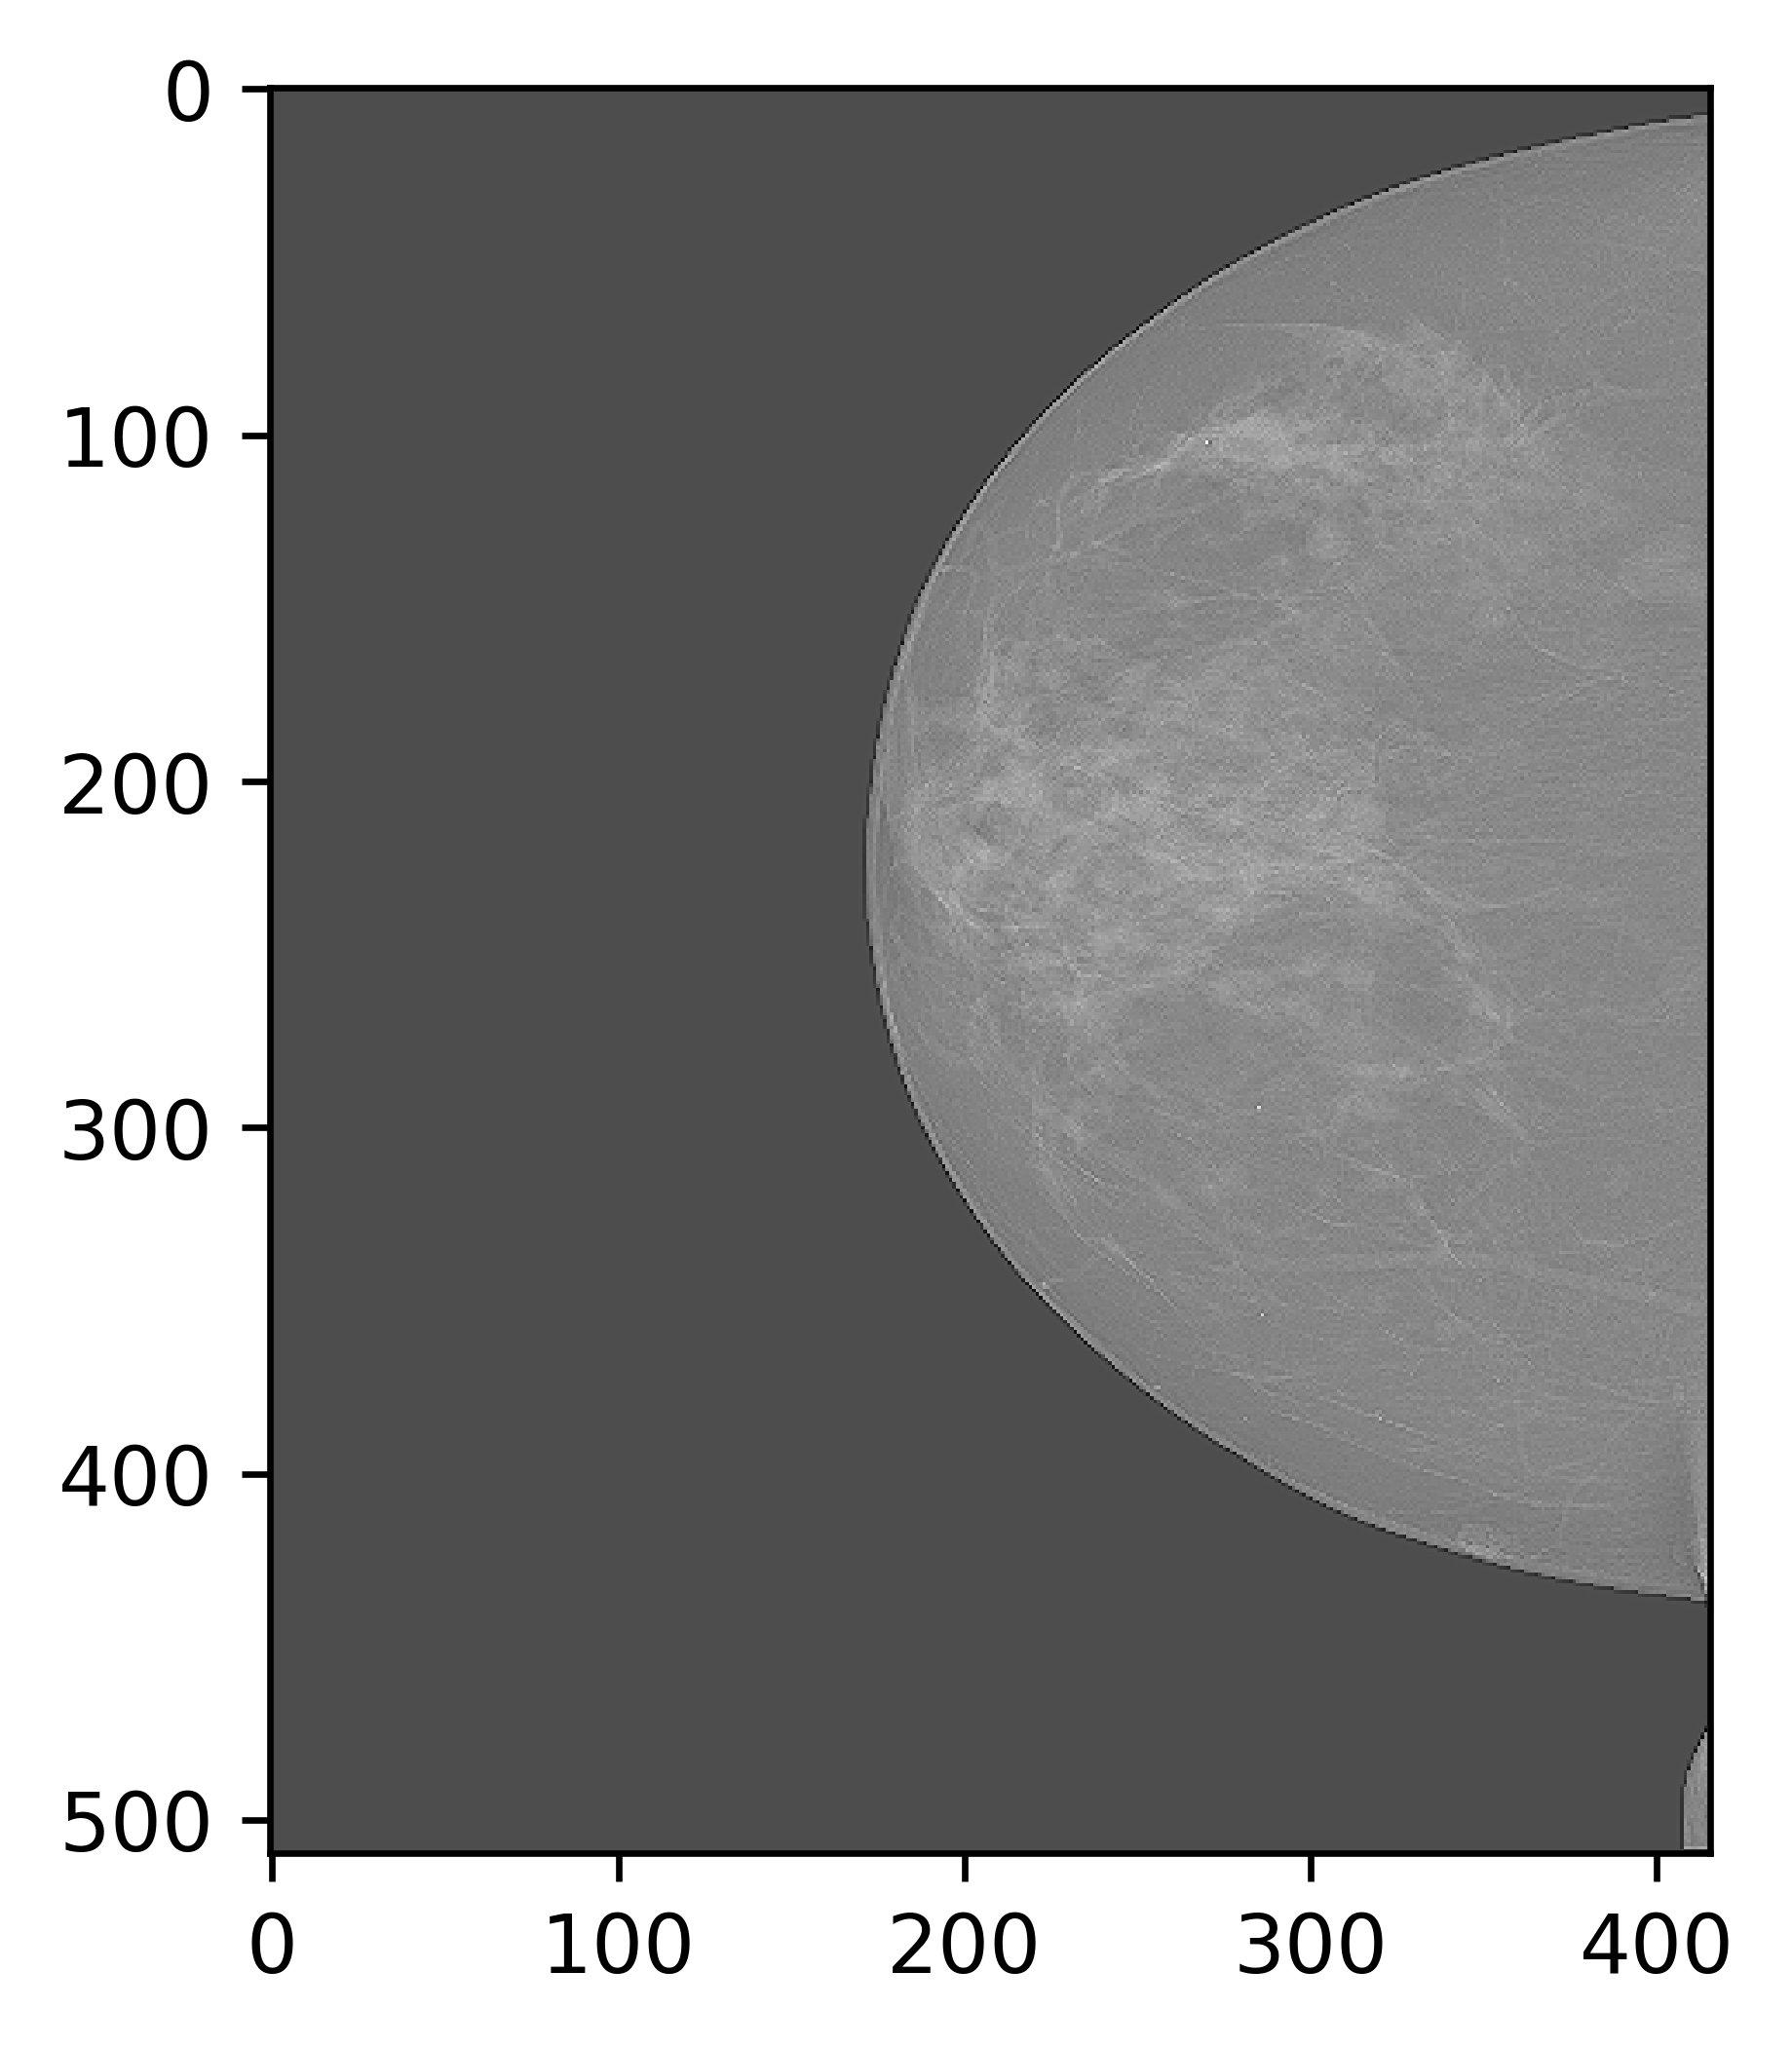
\includegraphics[width=\linewidth]{Graphics/mm-fusion.png}\par
\end{multicols}
\caption{Ejemplo de mamografía } \label{fig:example-mm}
\end{figure*}


\begin{figure}
	\centering
	\subfigure[ ]{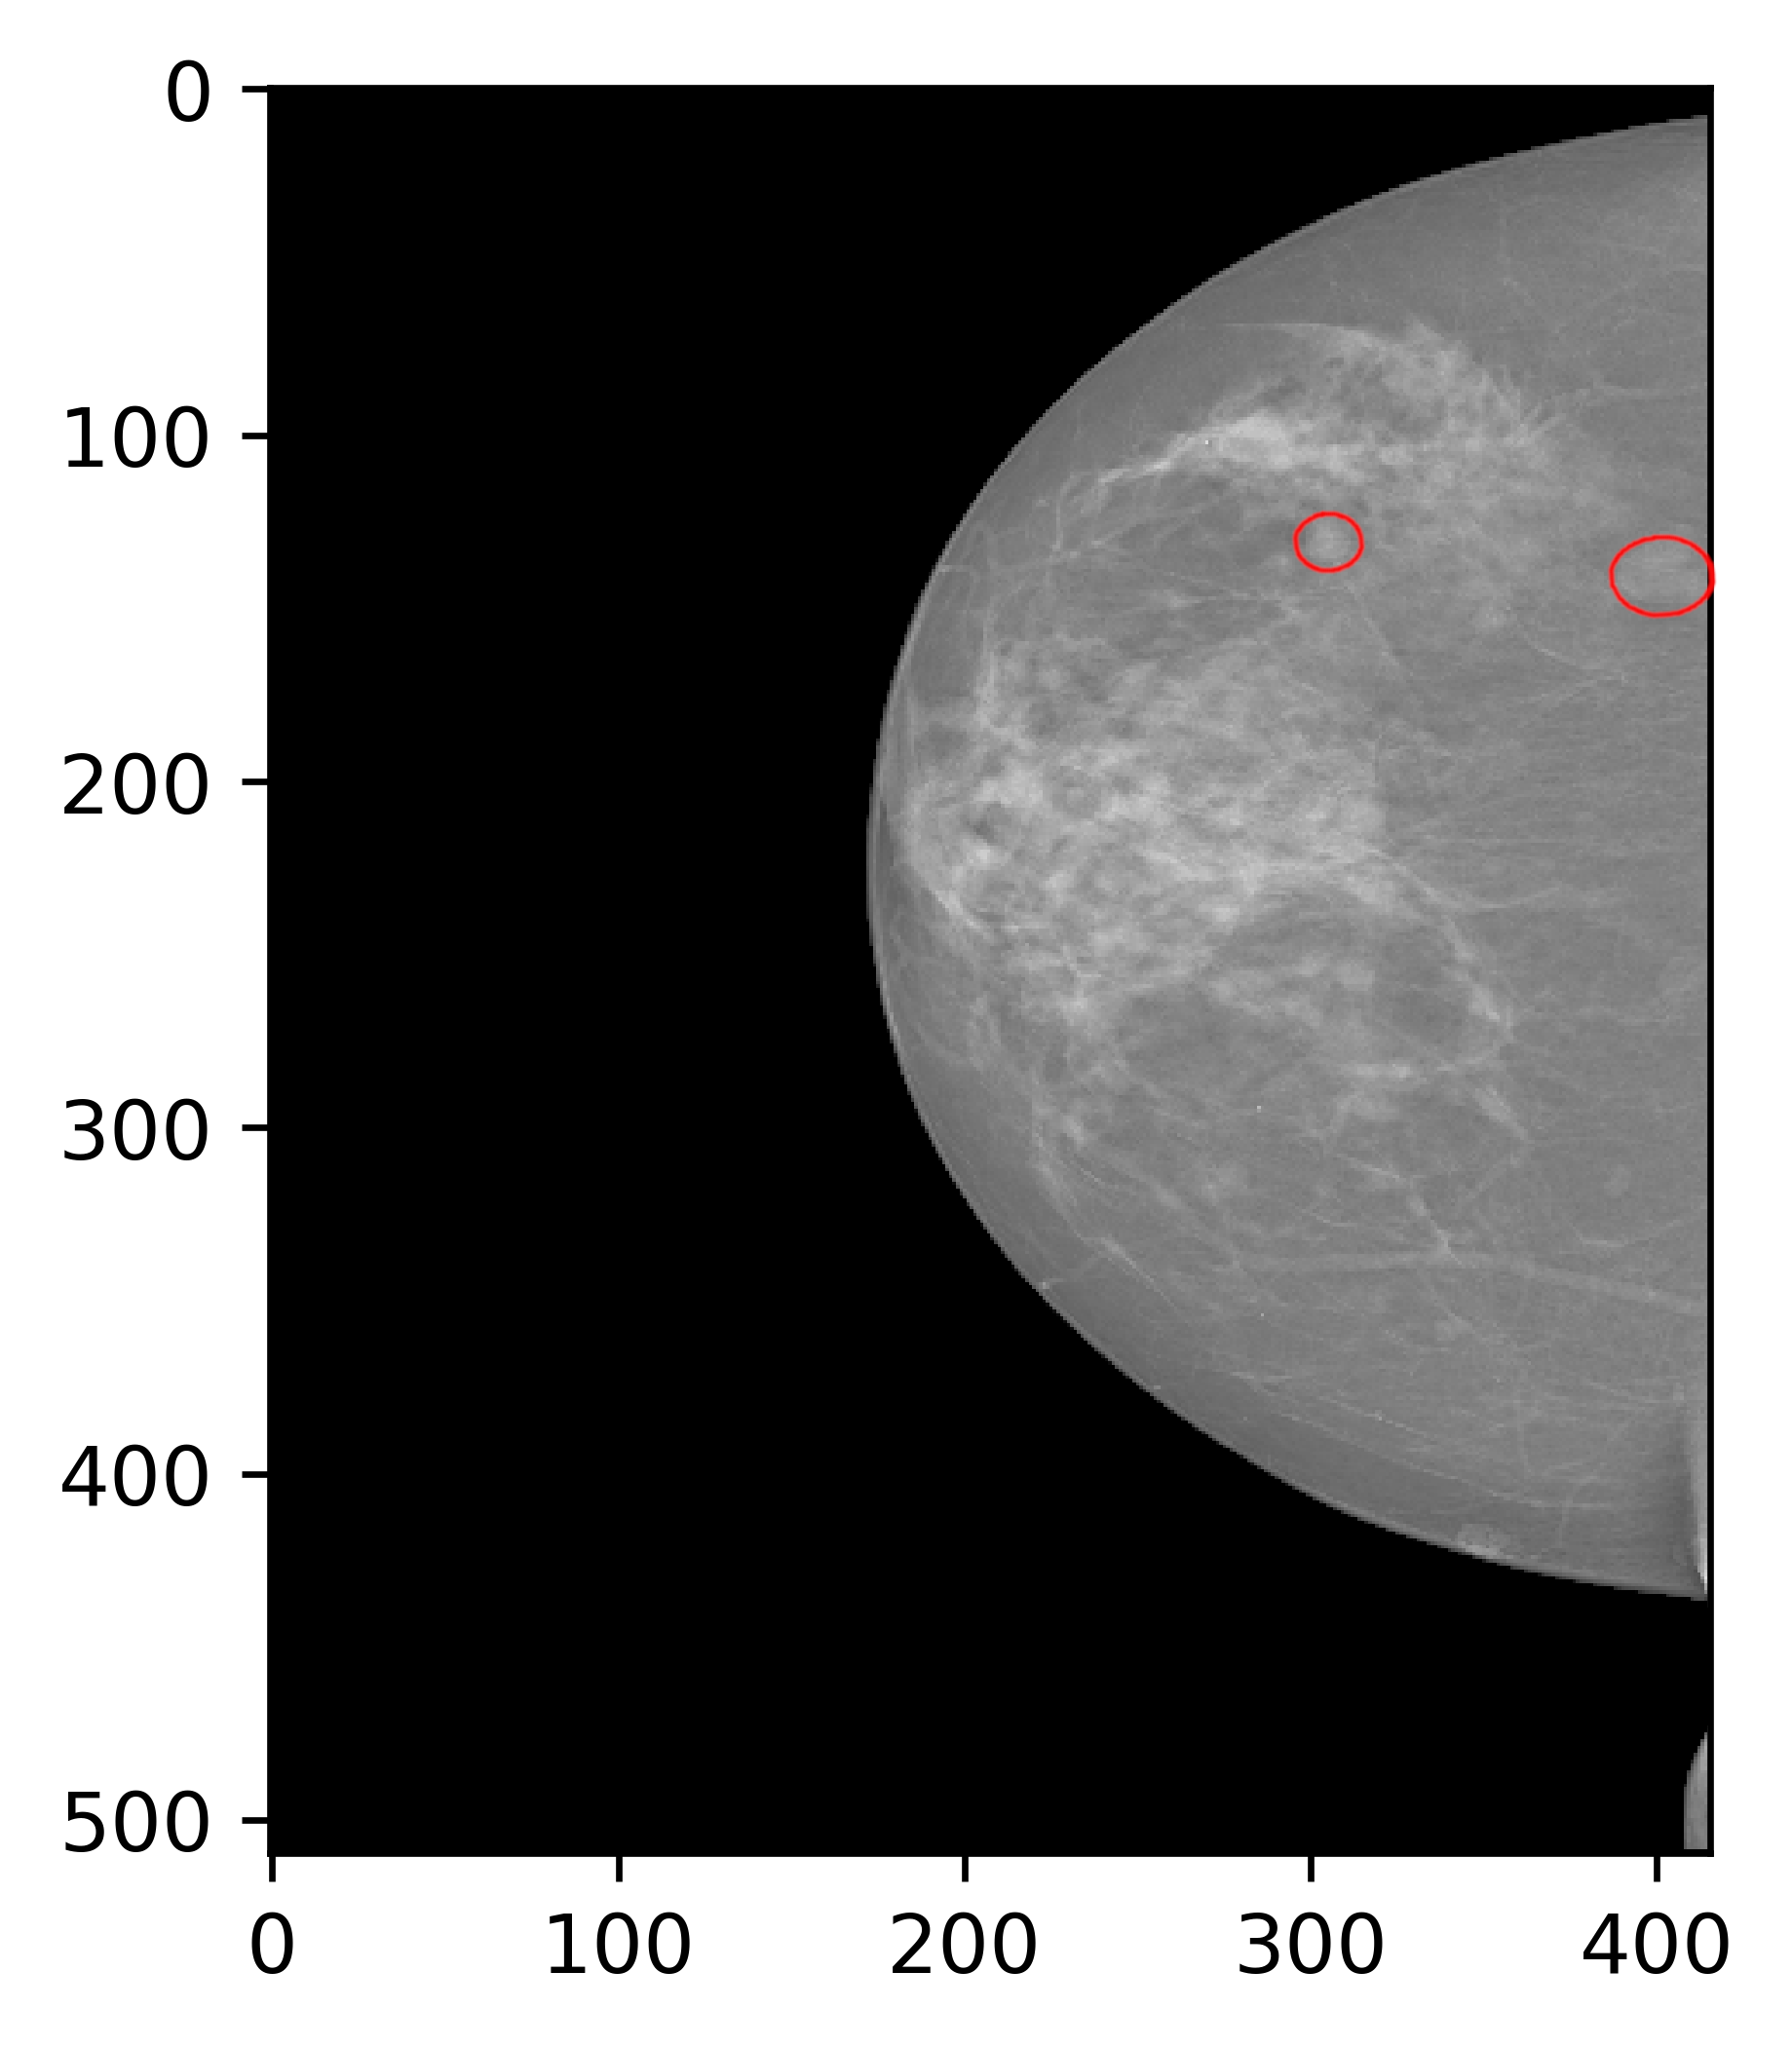
\includegraphics{Graphics/mm-rescaled-mass.png}}
	\subfigure[ ]{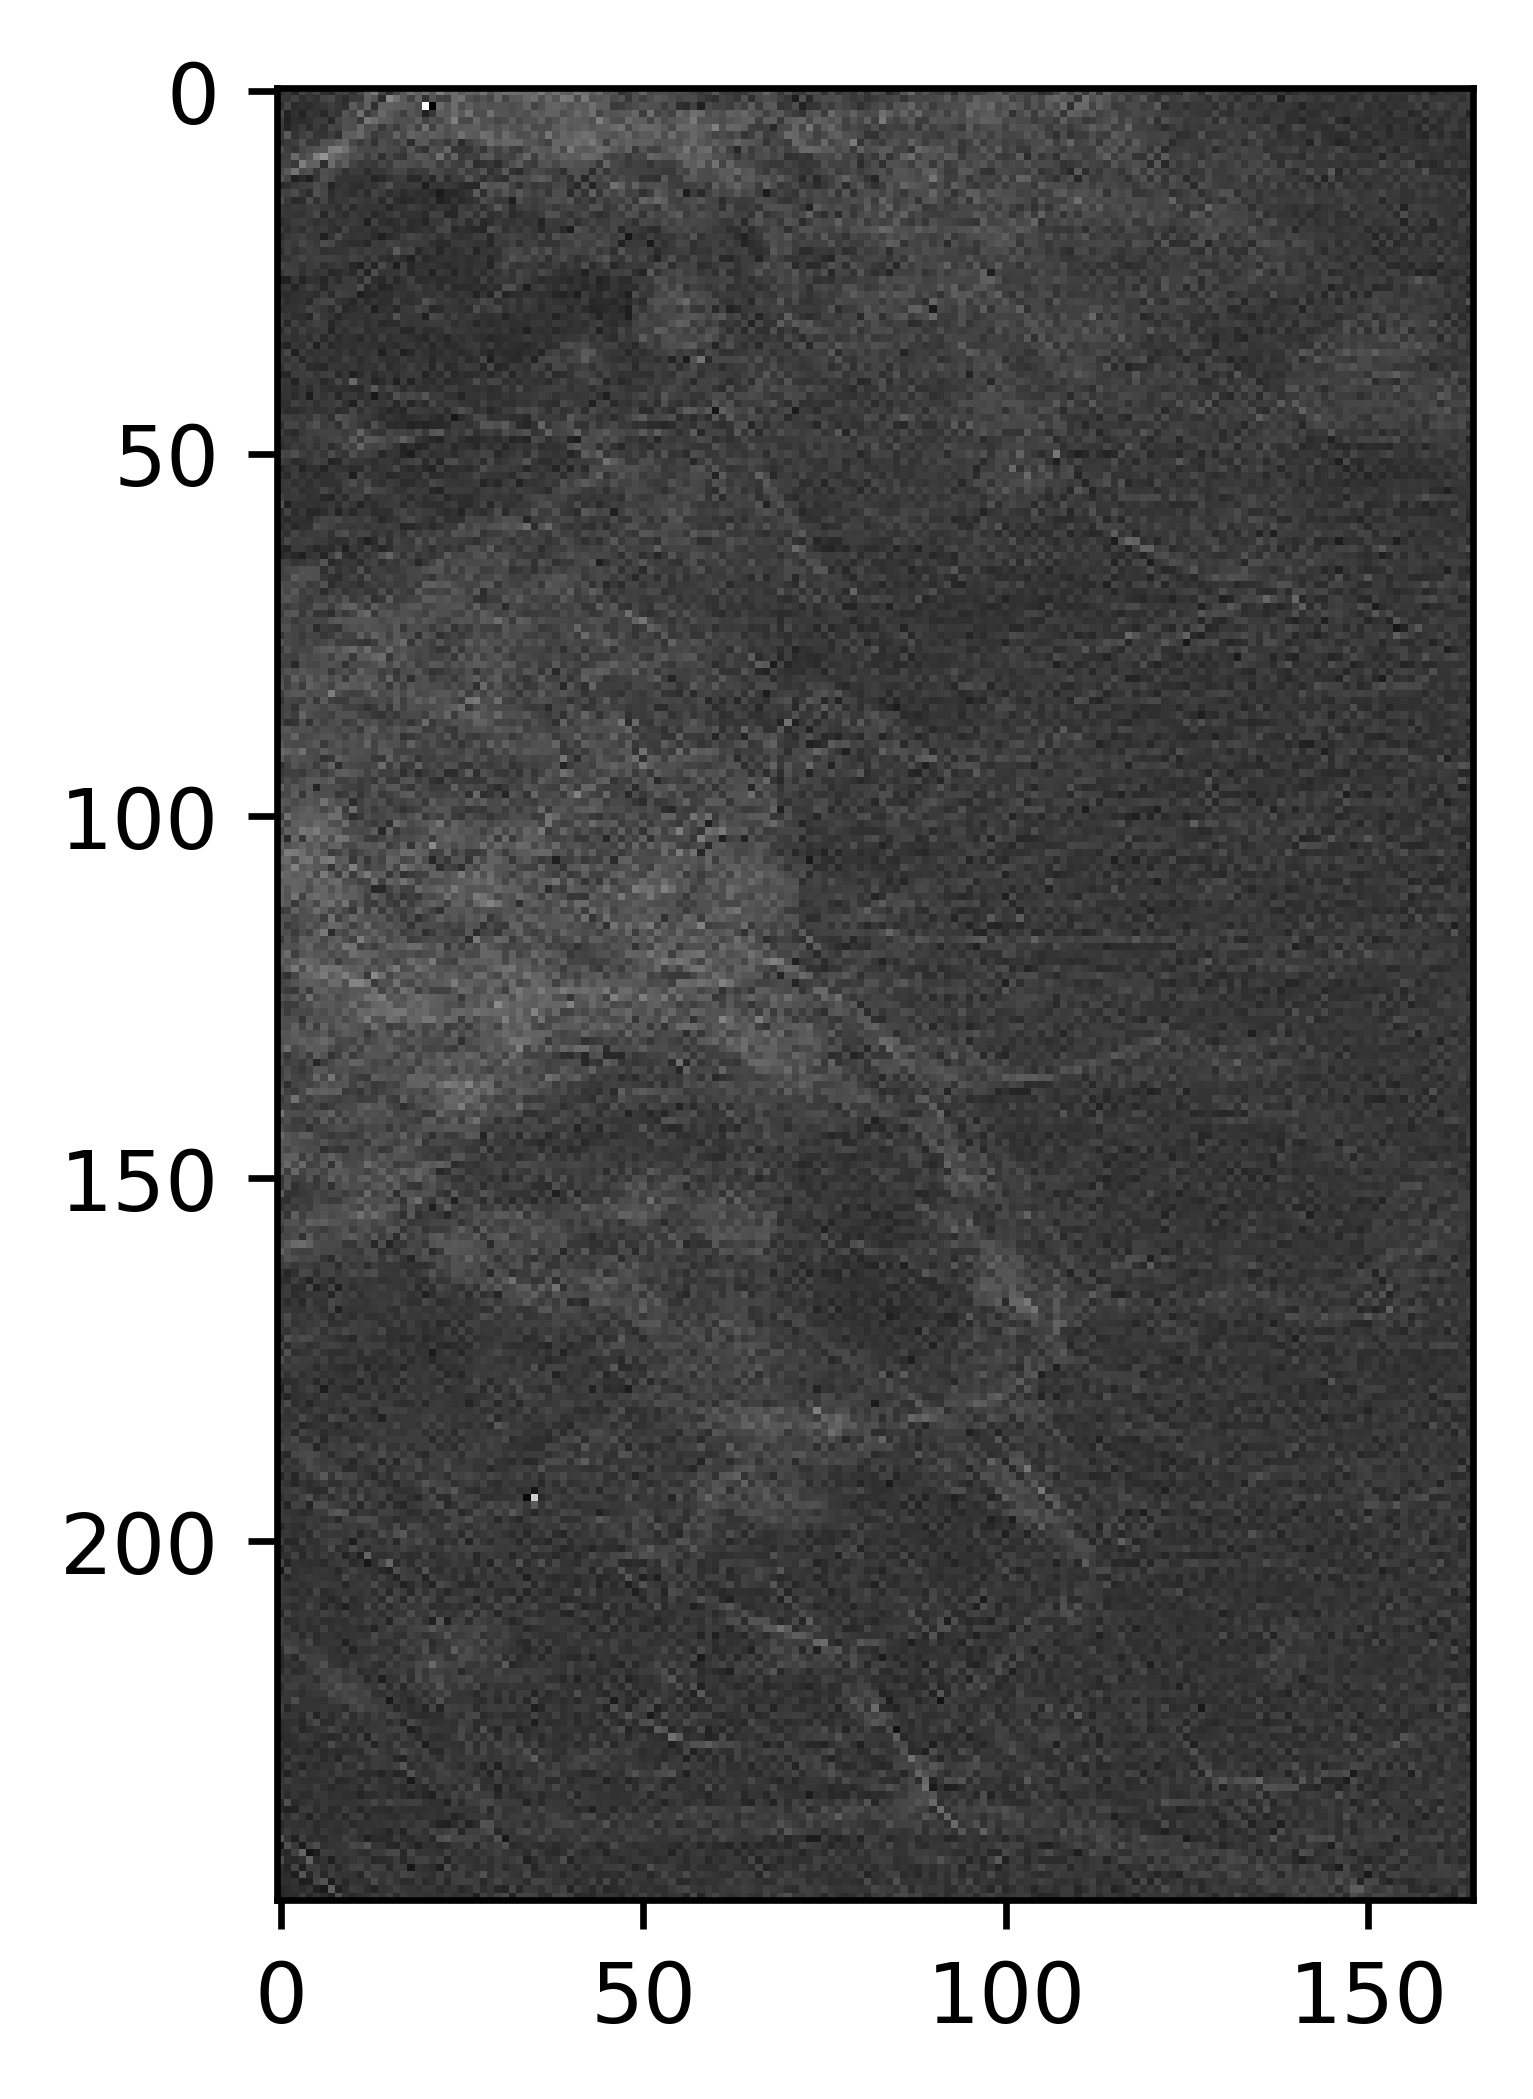
\includegraphics{Graphics/mm-portion.png}}
	\caption{} \label{fig:example-mm-portion}
\end{figure}

En la imagen de ejemplo existen dos masas. Pero solo se toma una para construir la shapelet(s), de esto modo se evalúa
la capacidad de responder del algoritmo para la detección de masas en general. En el caso ideal debería detectar ambas
regiones. Otro aspecto importante, es que para el experiemnto se toma una sección de la mamografía, donde no se contiene
el fondo negro, debido a que el mismo introduce muchos falsos positivos por el hecho de que los píxeles sean iguales 
cero. La figura \ref{fig:example-mm-portion} muestra la ubicación de las masas y la porción de la mamografía sobre
la cual se realiza el algoritmo de detección. La primera izquierda a derecha es la seleccionada para construir
la(s) shapelet(s).

\begin{figure*}
\begin{multicols}{2}
    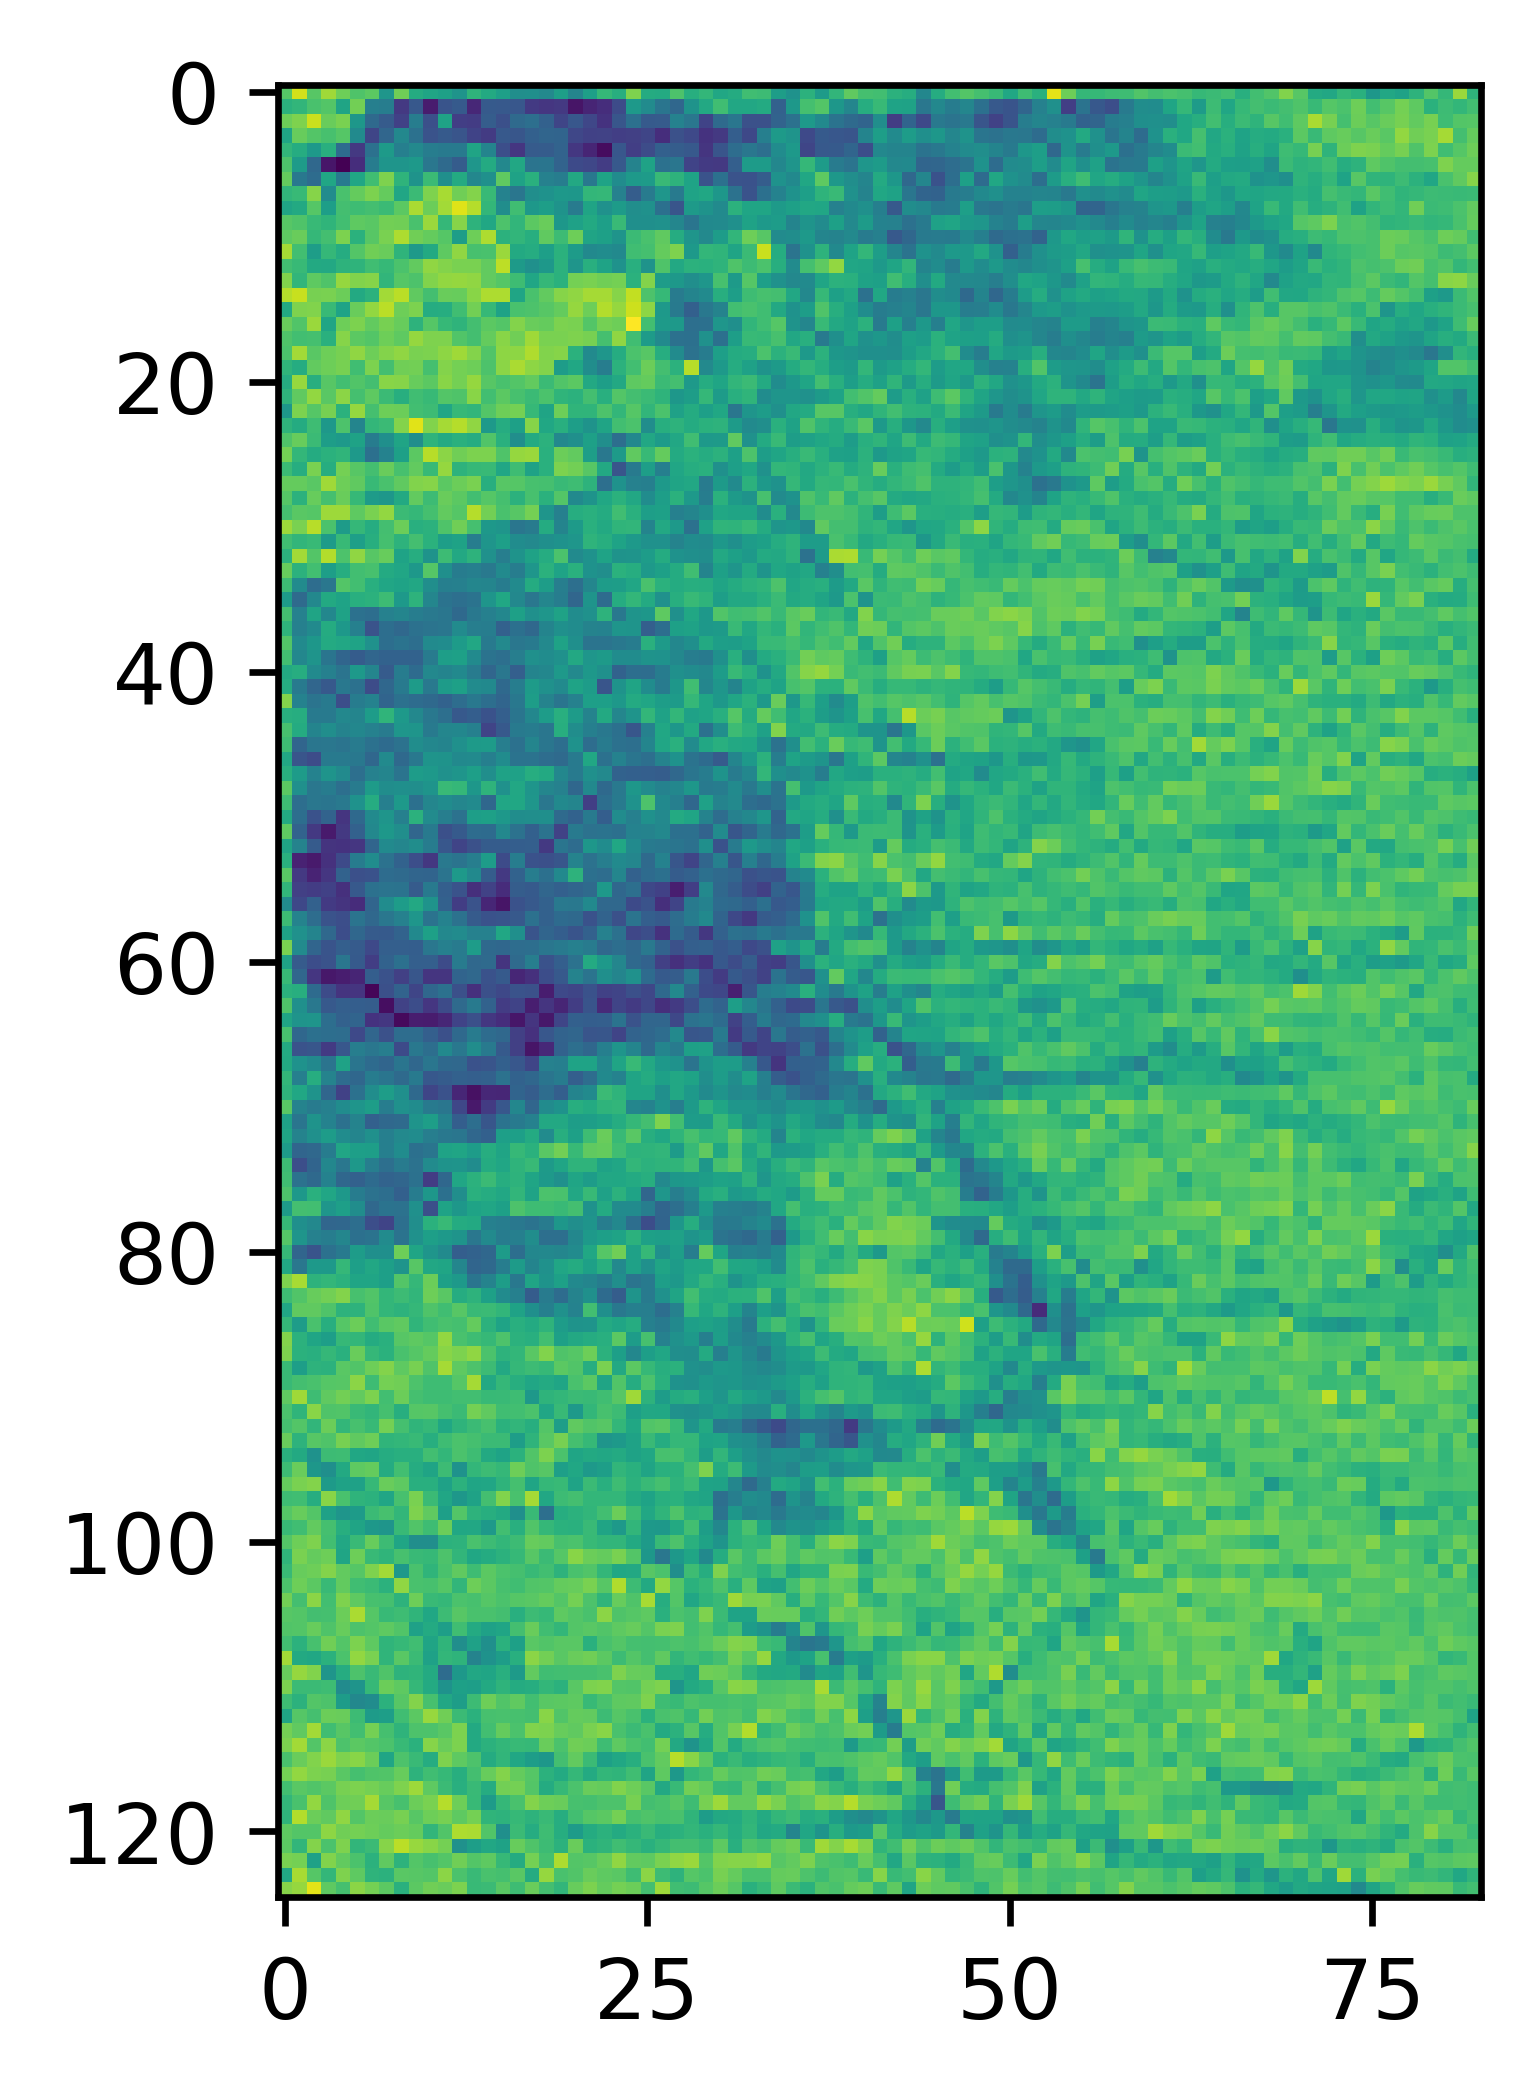
\includegraphics[width=\linewidth]{Graphics/mm-aprox.png}\par 
    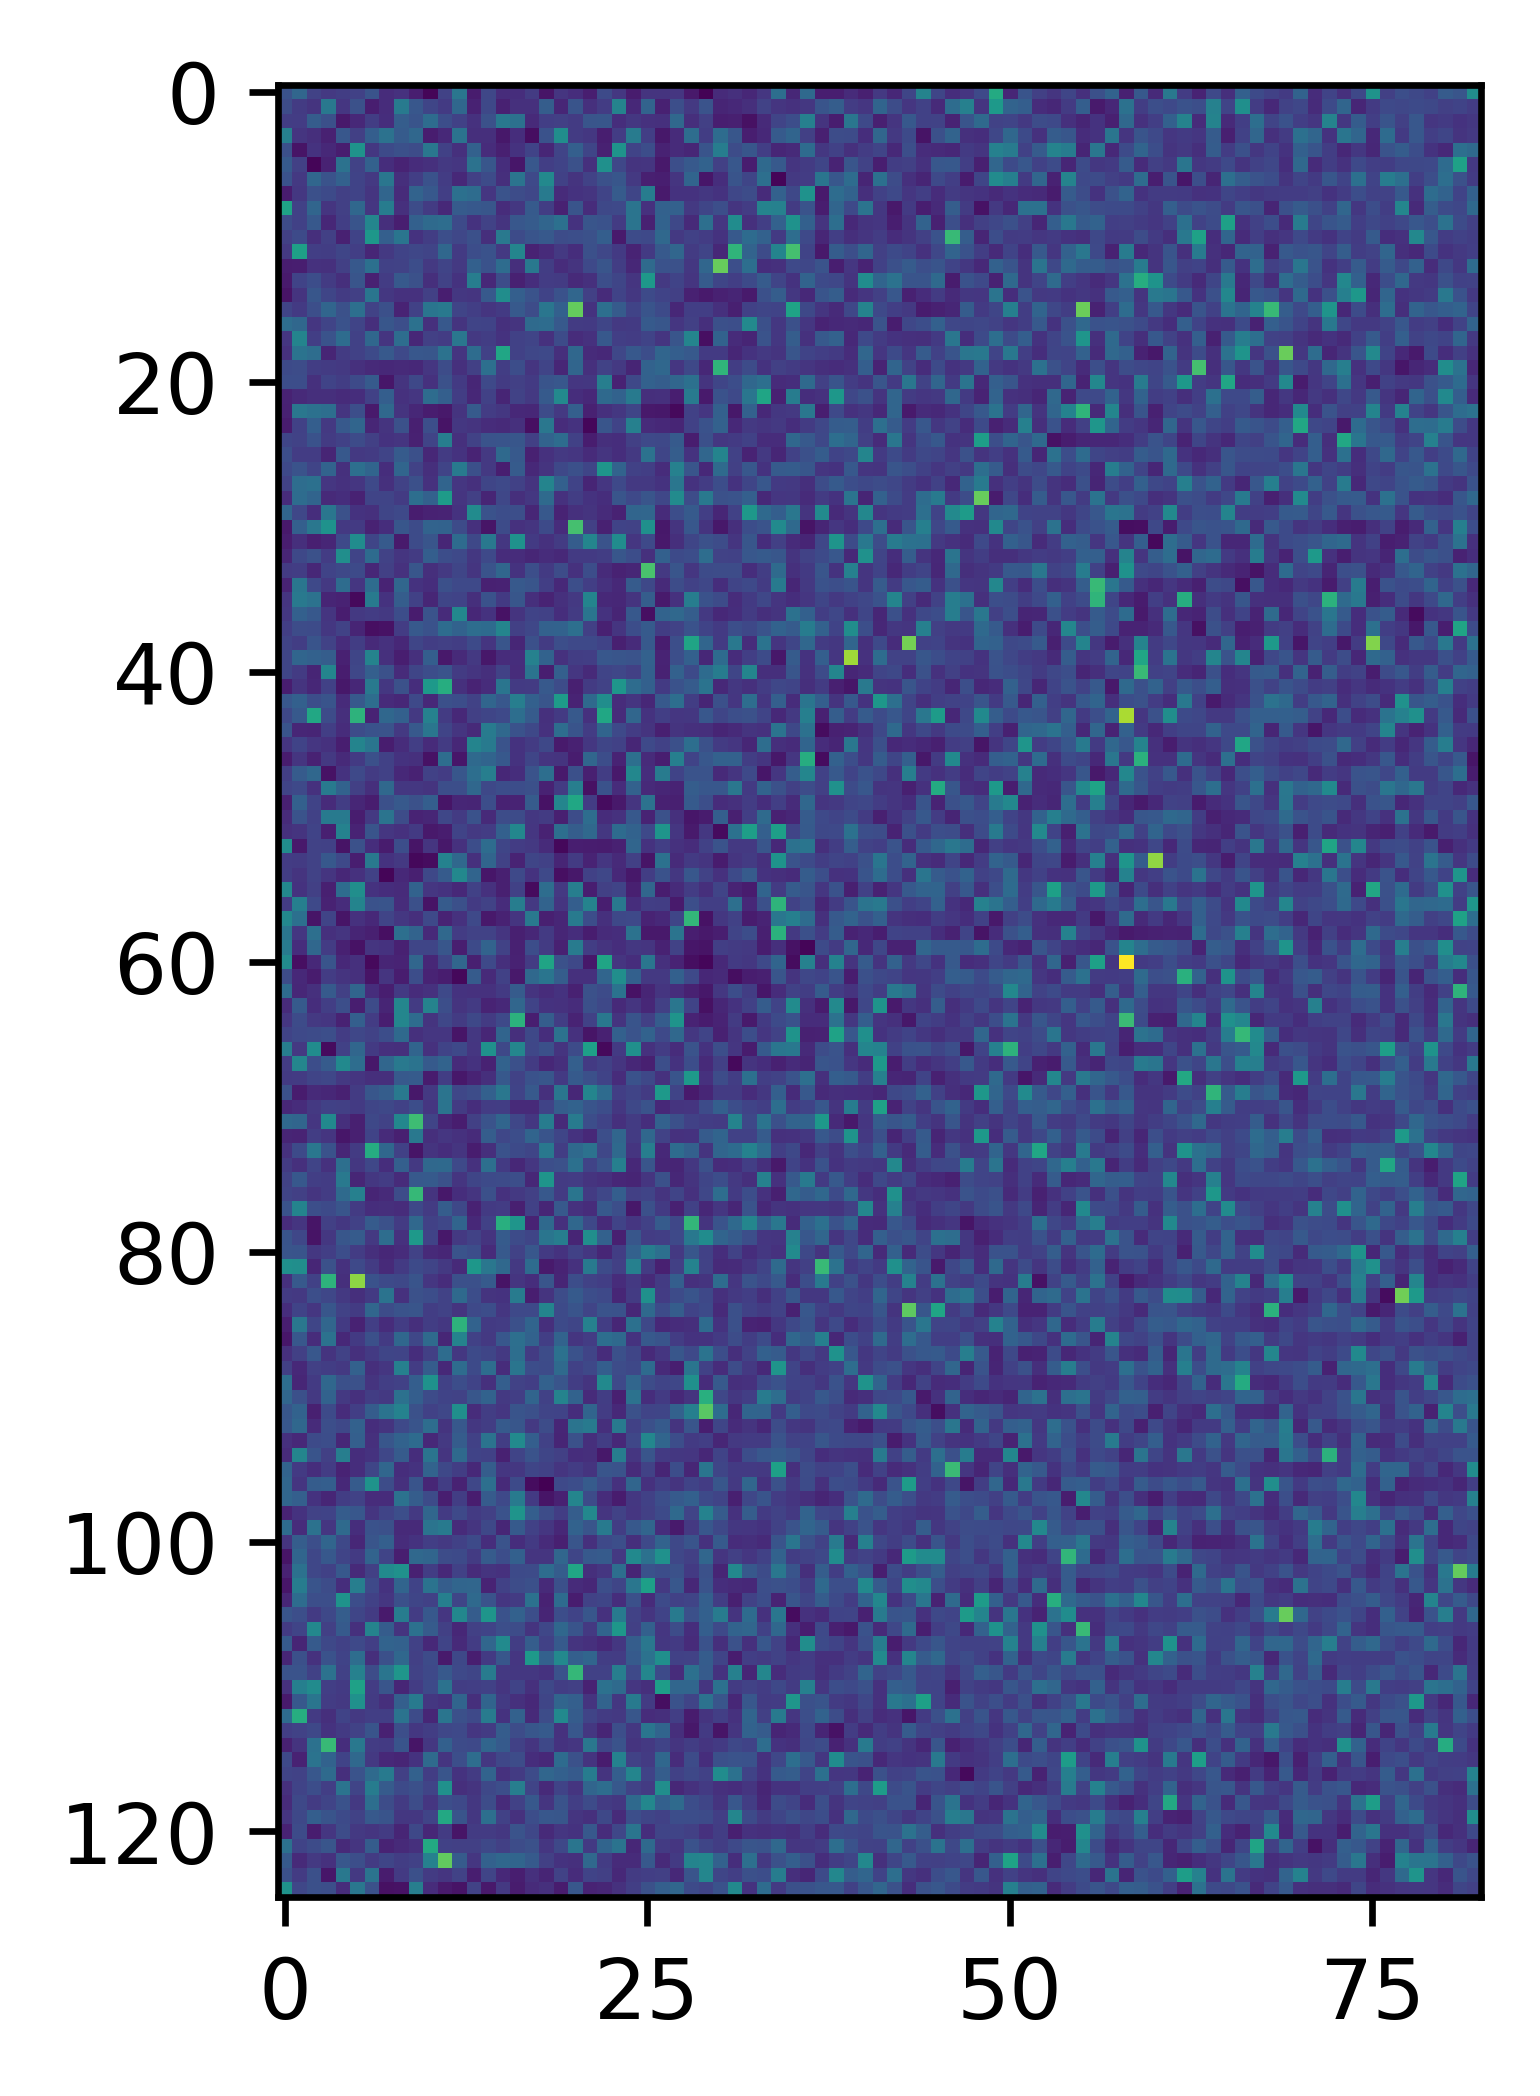
\includegraphics[width=\linewidth]{Graphics/mm-horizontal.png}\par 
    \end{multicols}
\begin{multicols}{2}
    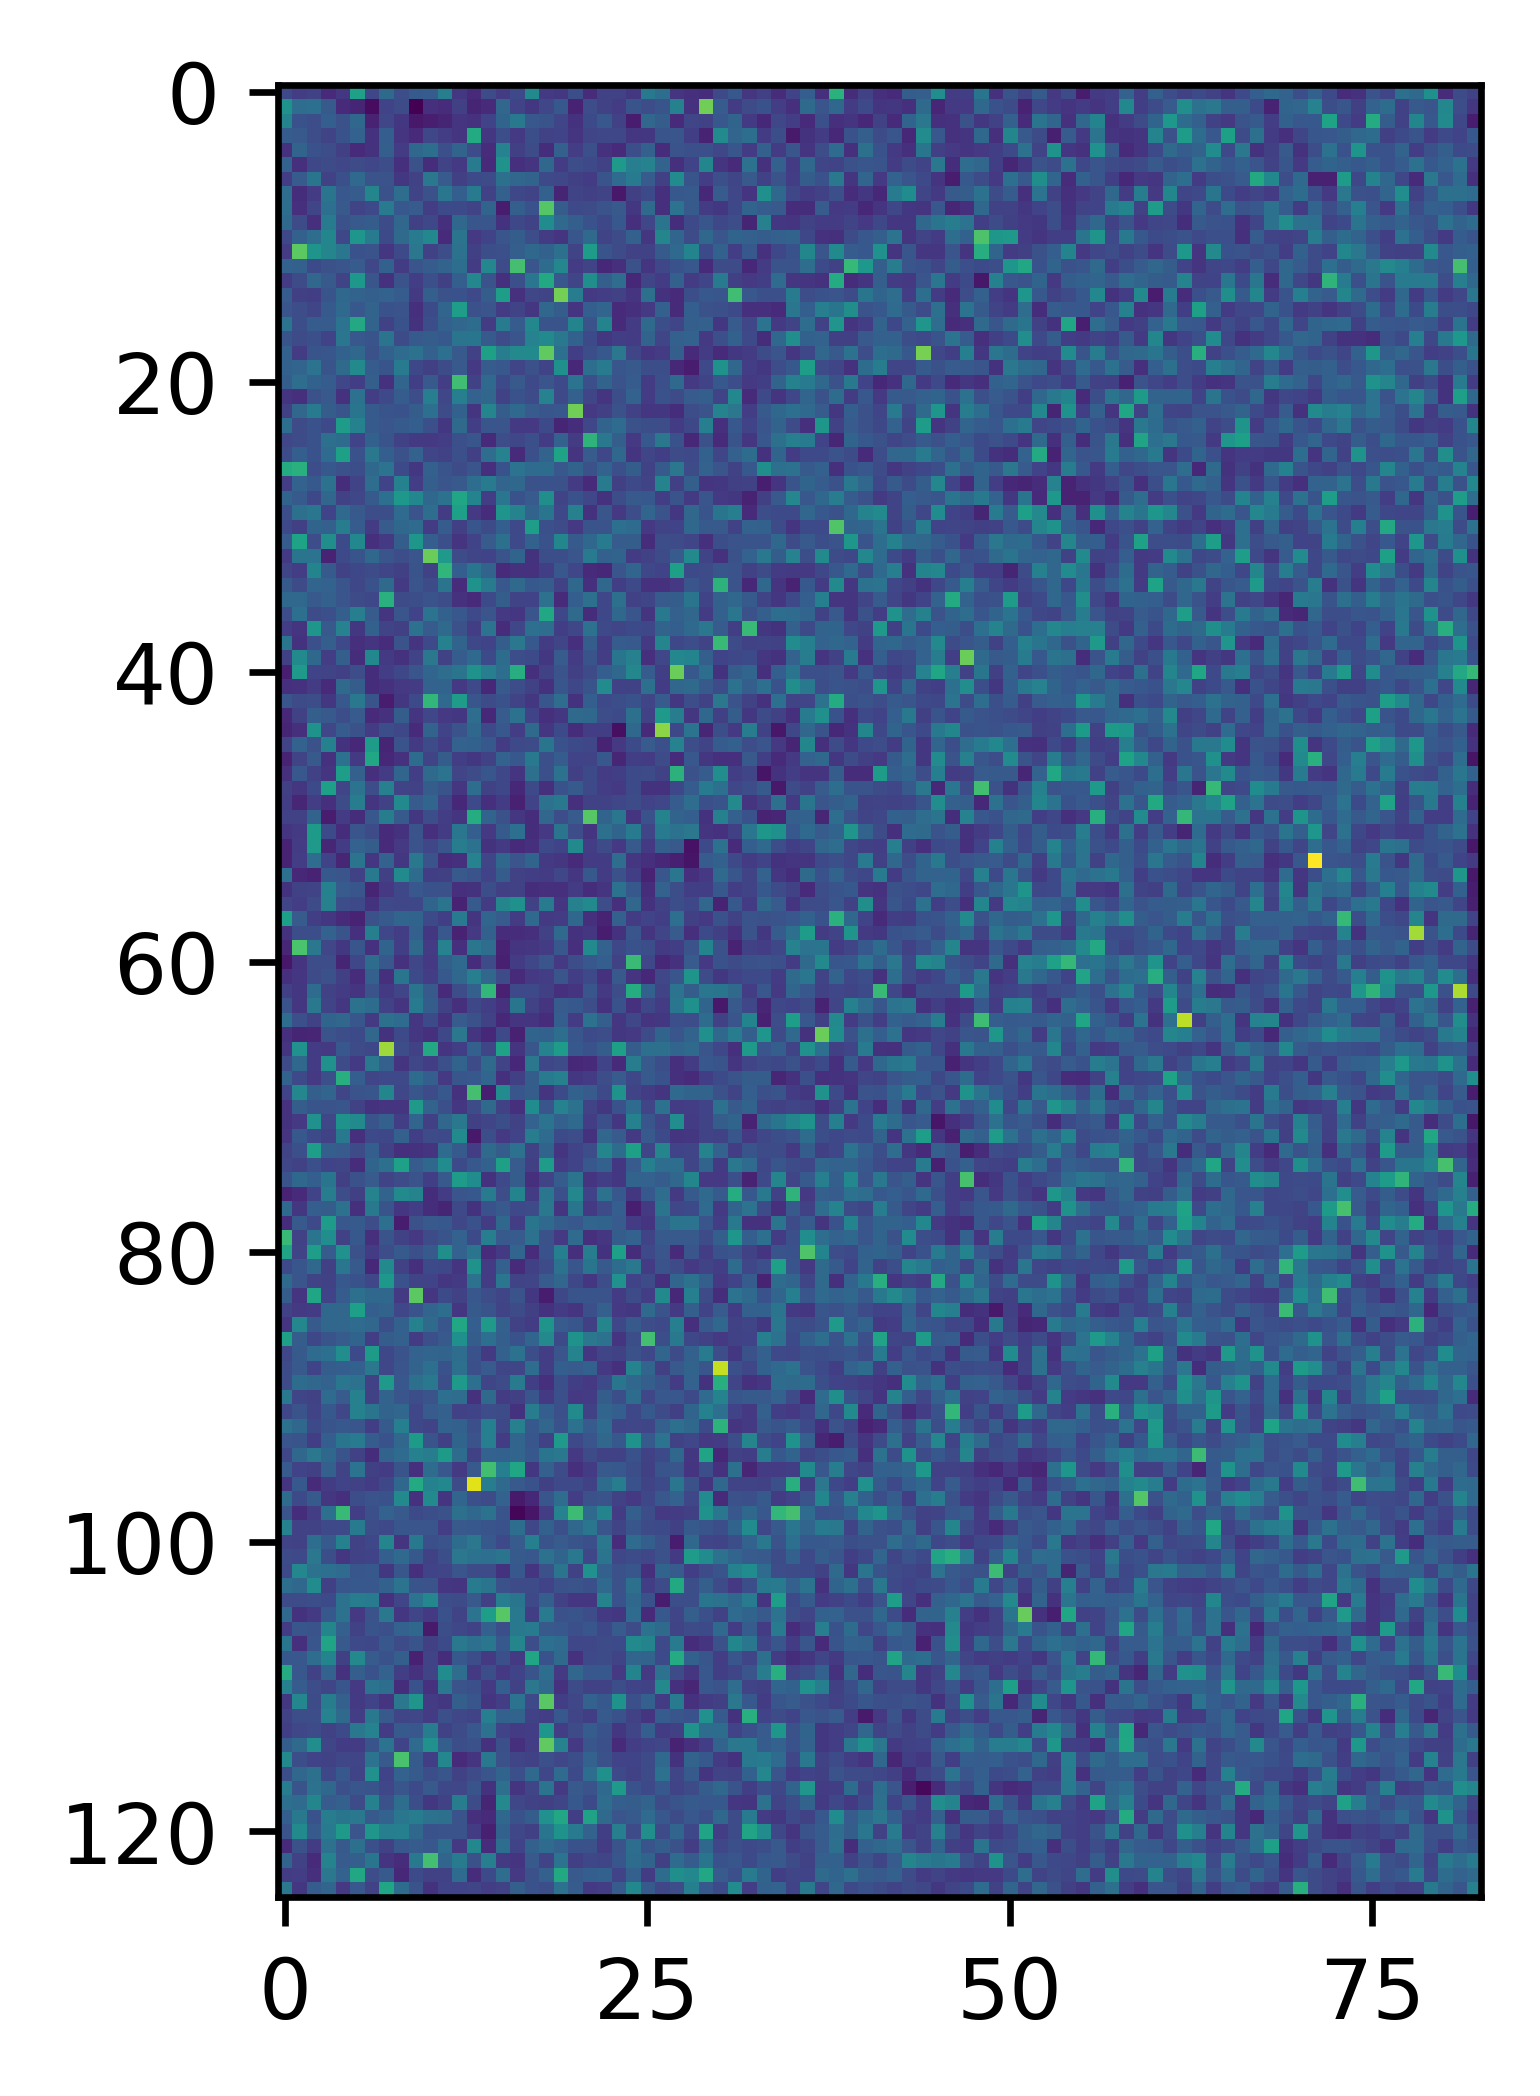
\includegraphics[width=\linewidth]{Graphics/mm-vertical.png}\par
    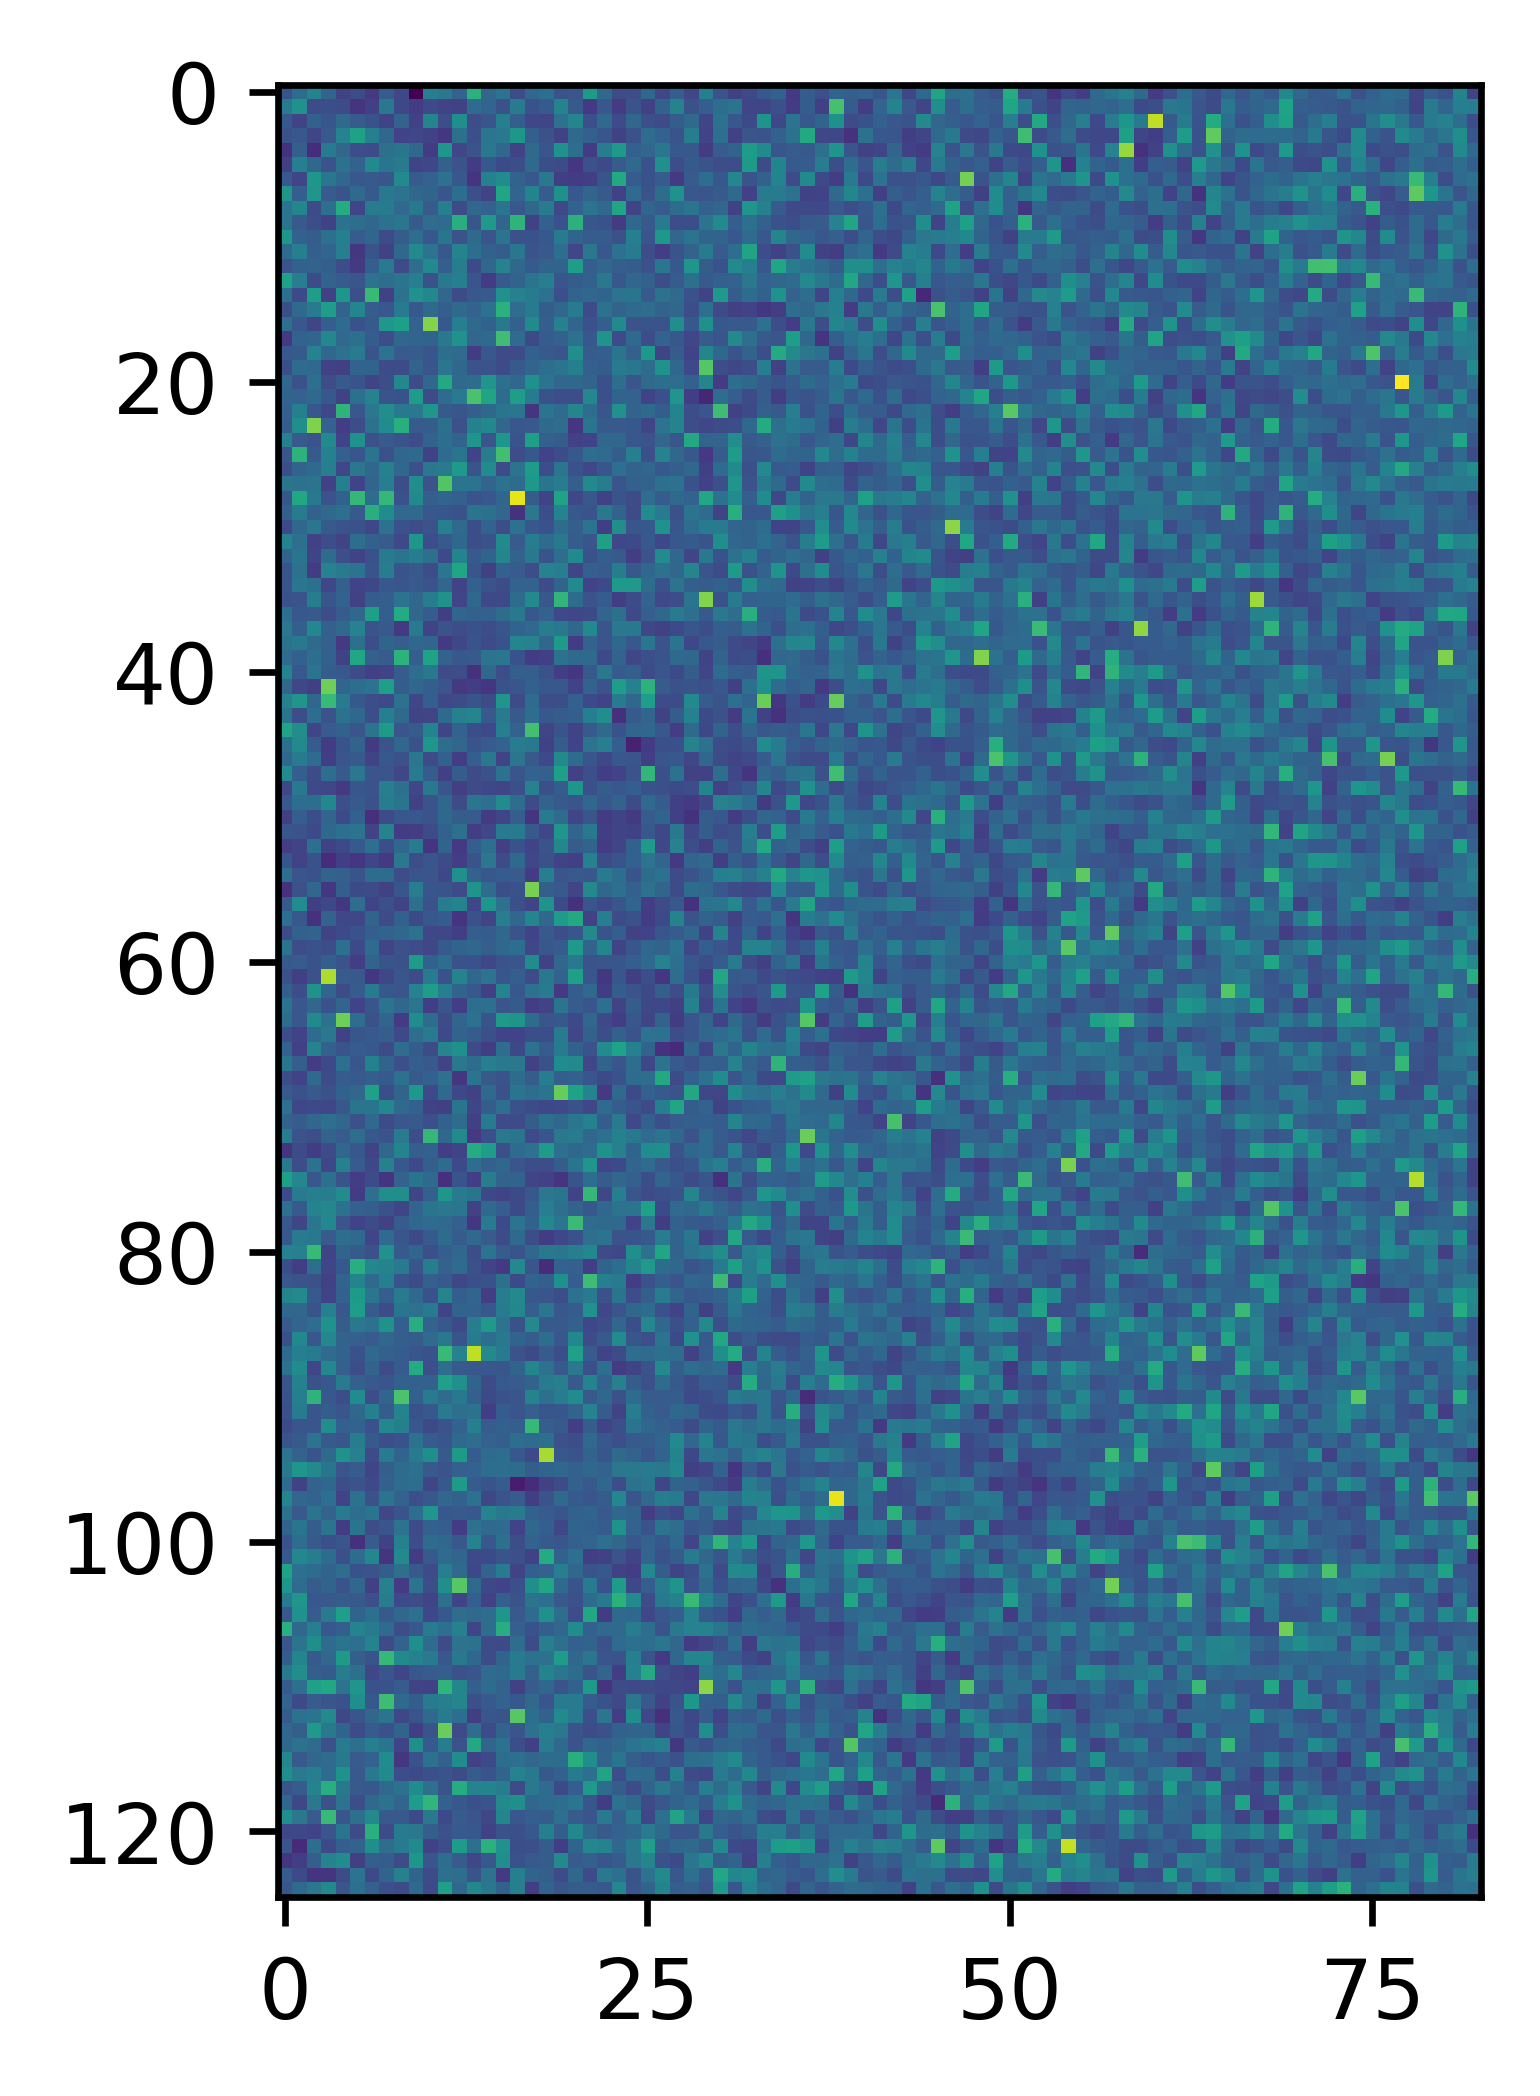
\includegraphics[width=\linewidth]{Graphics/mm-diagonal.png}\par
\end{multicols}
\caption{} \label{fig:example-mm-approach1}
\end{figure*}

El resultado del primer enfoque se muestra en la figura \ref{fig:example-mm-approach1}. Como se puede tanto en este caso como en el
del ejemplo de la gaussiana no hay ningún signo de detección. Esto refuerza aún más la conclusión de que la DST-II no se puede
extender para el caso 2D con este enfoque.

\begin{figure}
	\centering
	\subfigure[ ]{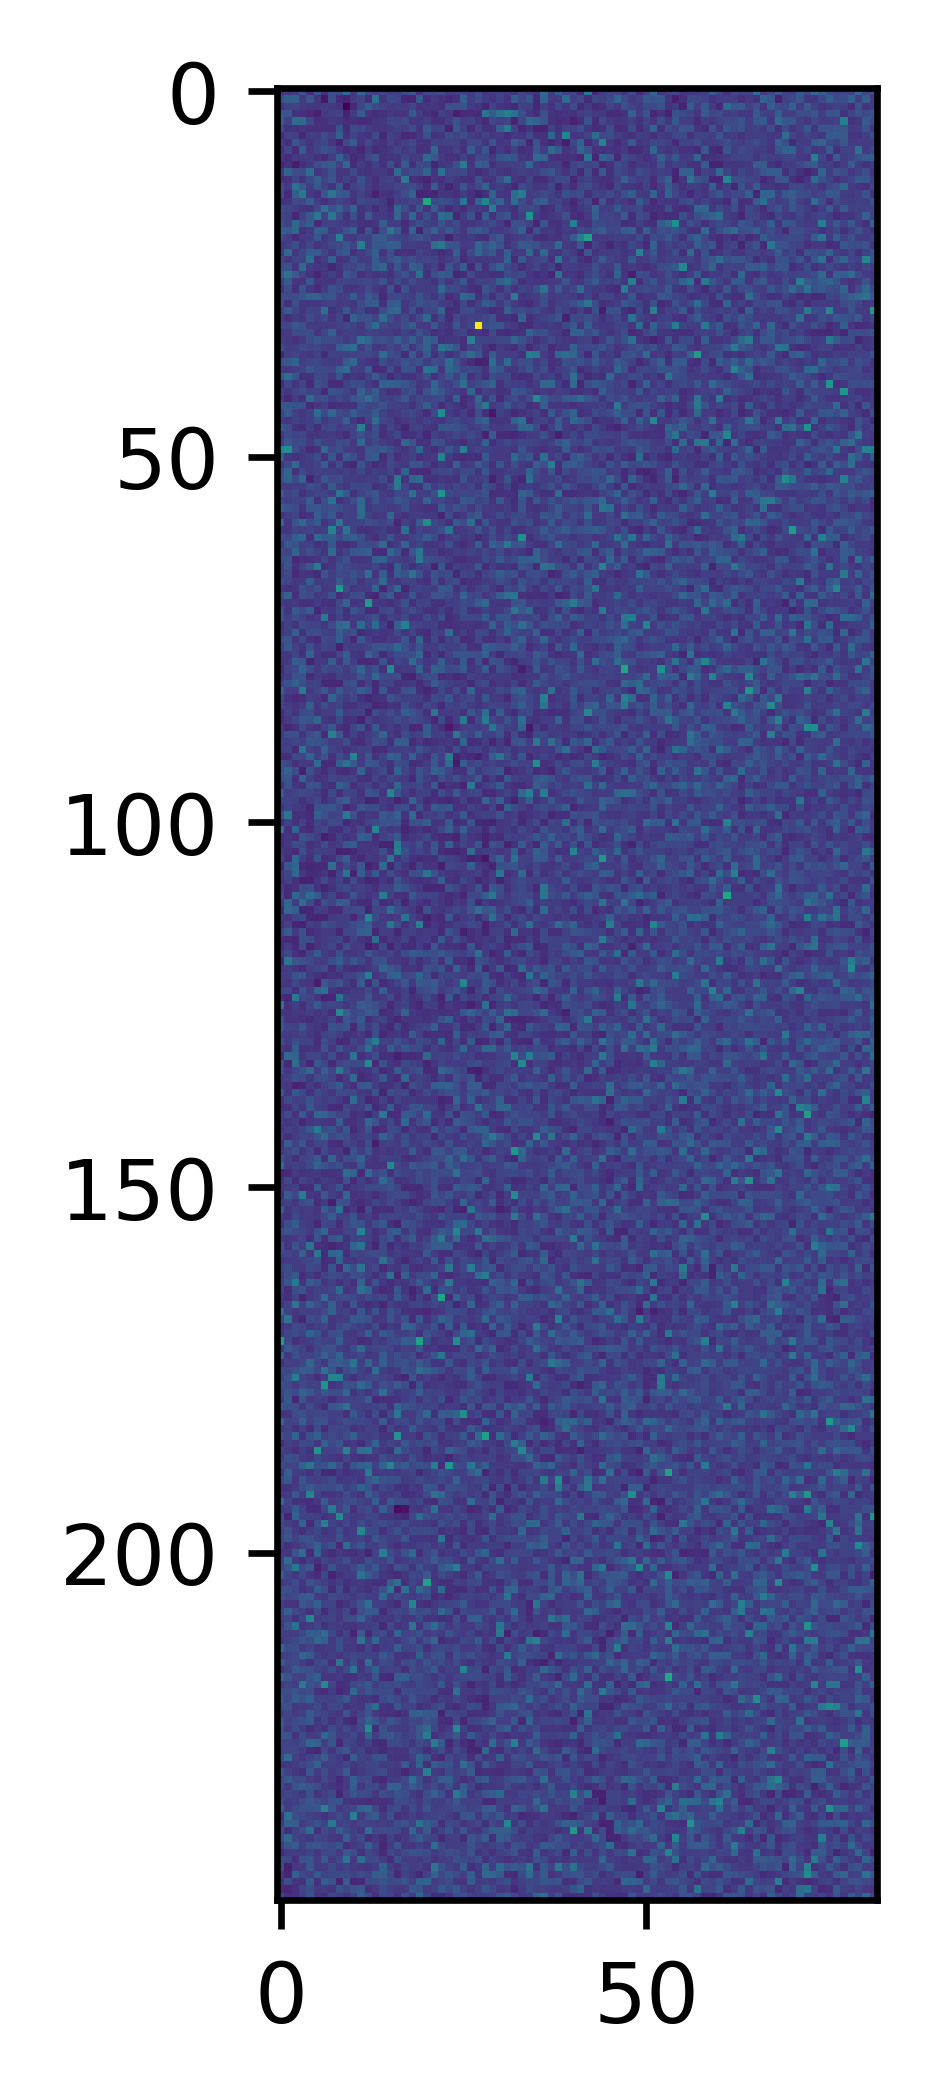
\includegraphics{Graphics/mm-row.png}}
	\subfigure[ ]{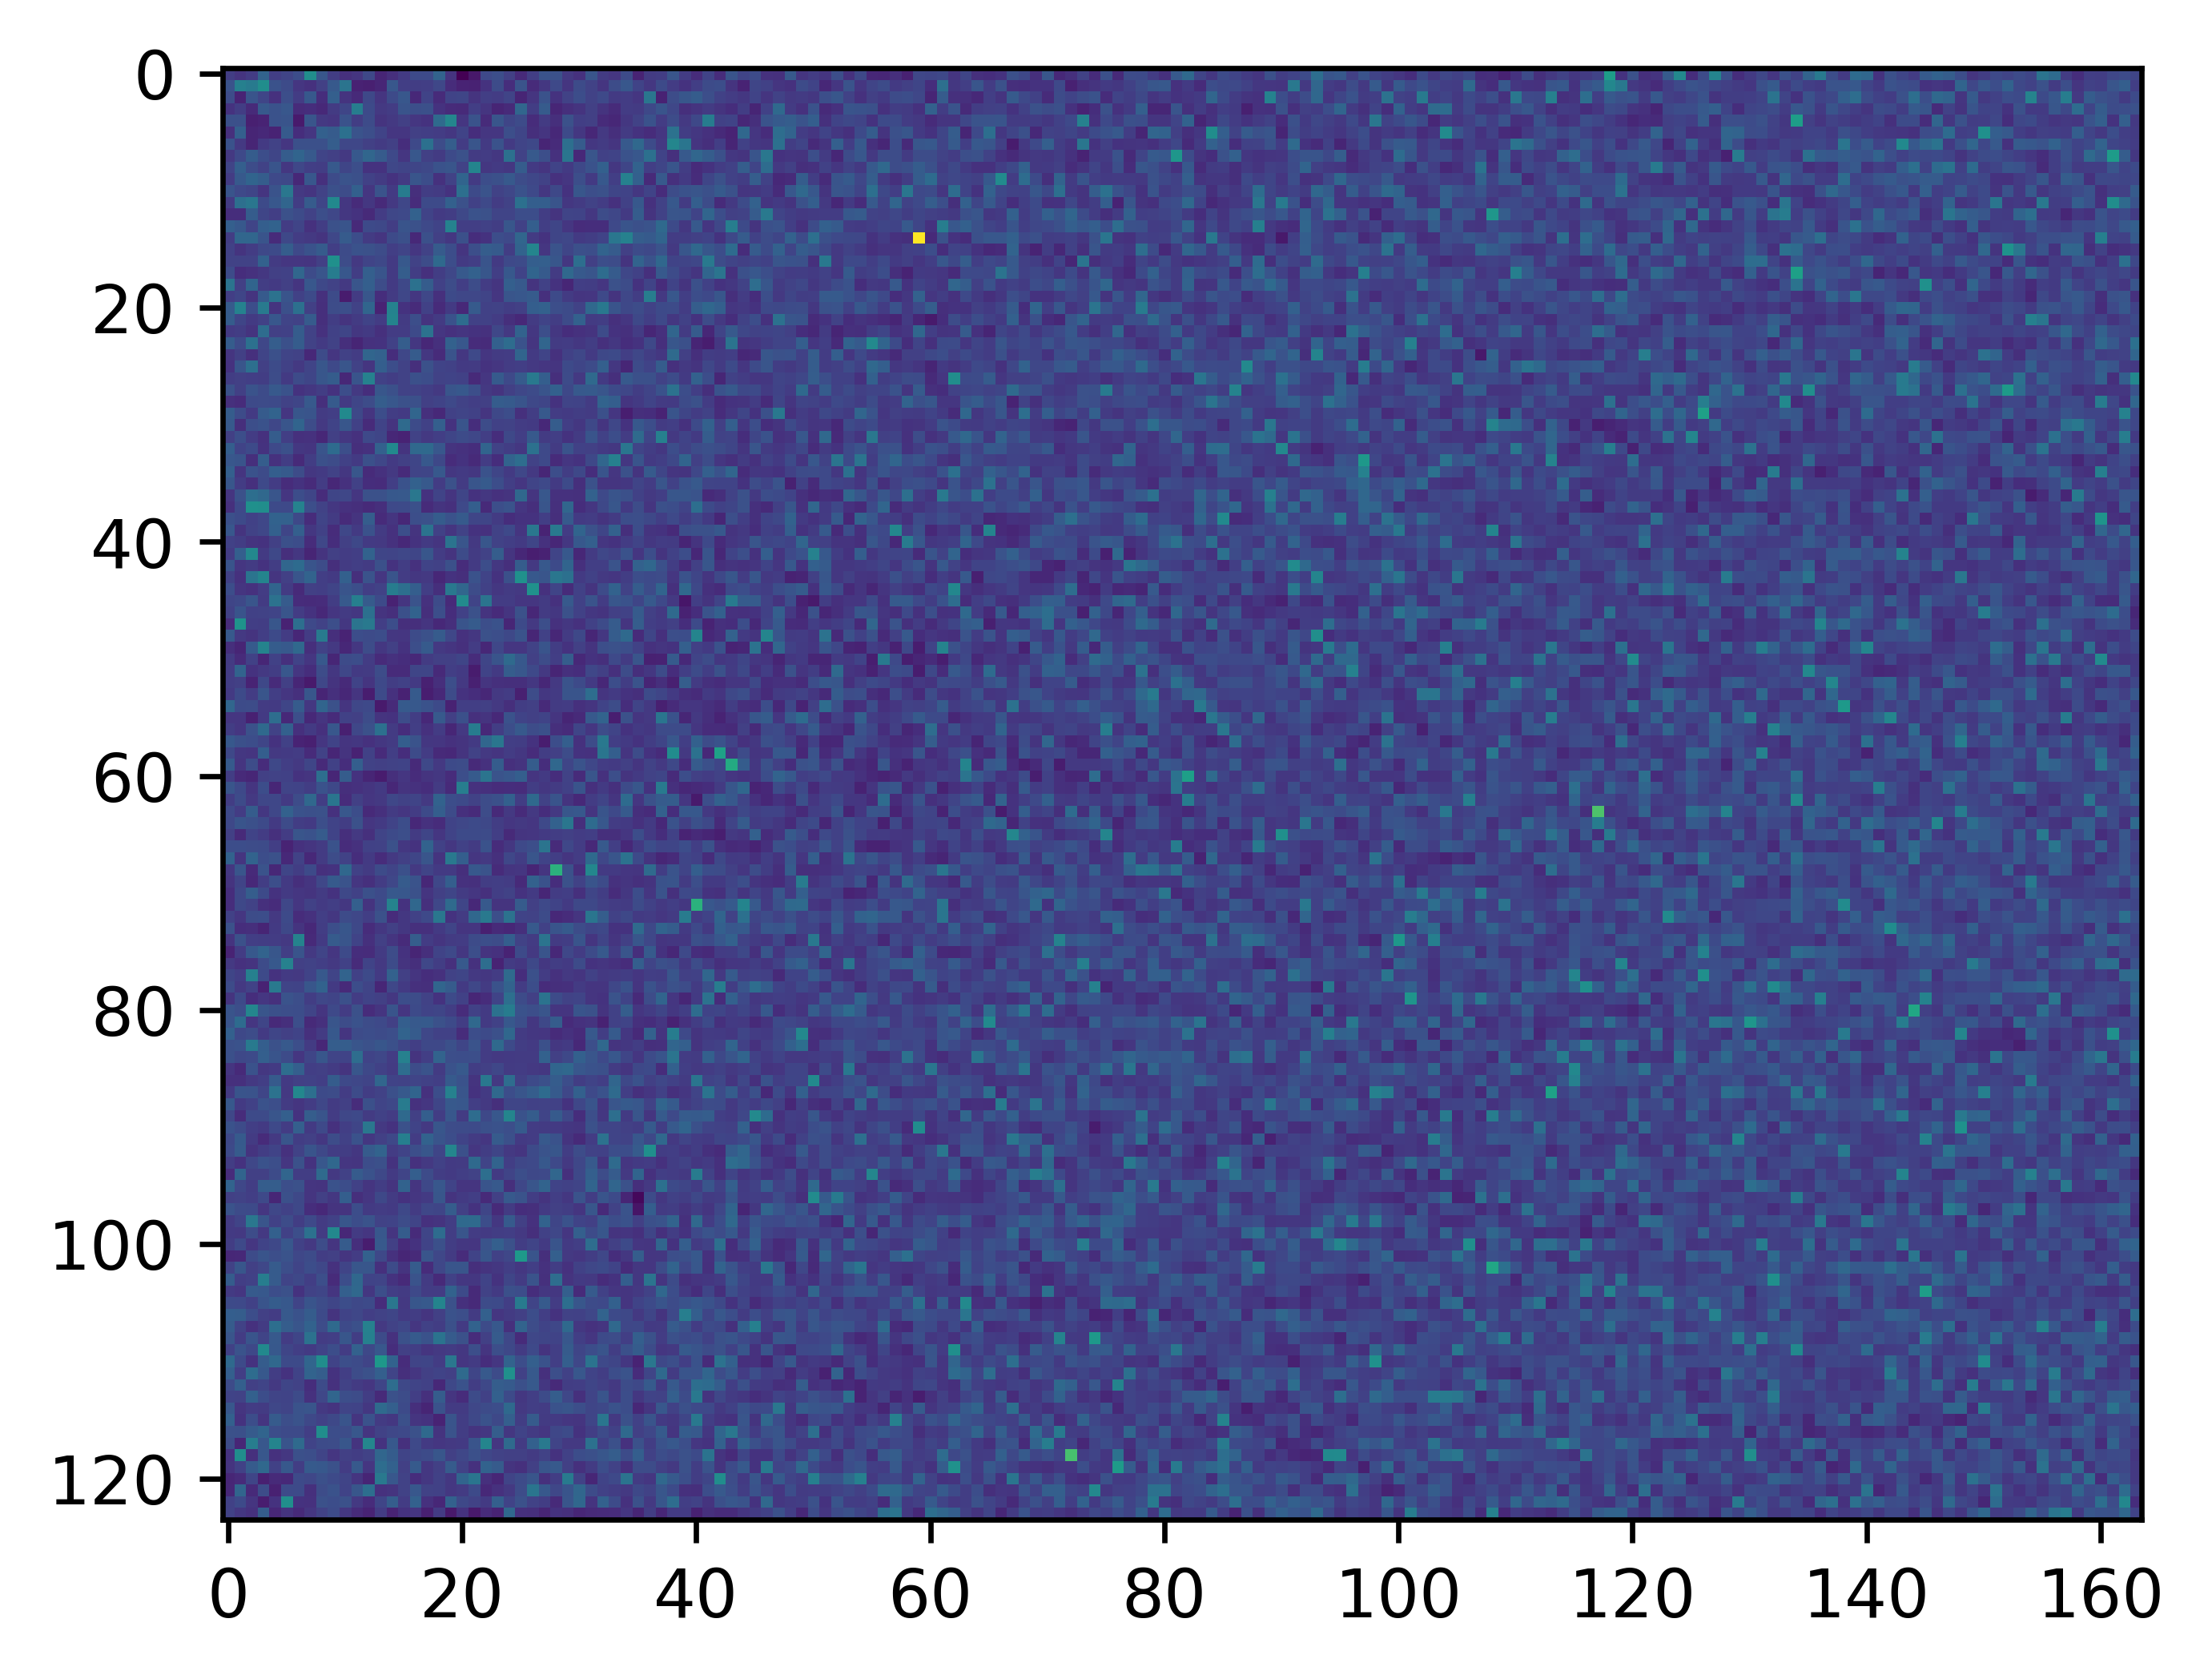
\includegraphics{Graphics/mm-col.png}}
	\caption{} \label{fig:example-mm-approach2}
\end{figure}
%Detection at position (32, 27) with value 0.9831863519468129 row
%Detection at position (14, 59) with value 0.983604207430764 col

En el caso del segundo enfoque  los resultados son mejores. Si se observa la figura \ref{fig:example-mm-approach2}, al menos hay signos de detección.
Aunque bien díficiles de ver, existen un par de píxeles, uno en cada imagen que constrastan con el resto.
Estos están ubicados en las posiciones $(32,27)$ y $(14,59)$ con valores $0.9831863519468129$ y $0.983604207430764$
respectivamente. Ambos corresponden a posiciones aproximadas $(32,54)$ y $(28,59)$, donde se encuentra el patrón extraído.
A pesar de que el segundo enfoque logra detectar la posición donde se encuentra el patrón, no detecta la segunda masa.

\begin{figure}
	\centering
	\subfigure[ ]{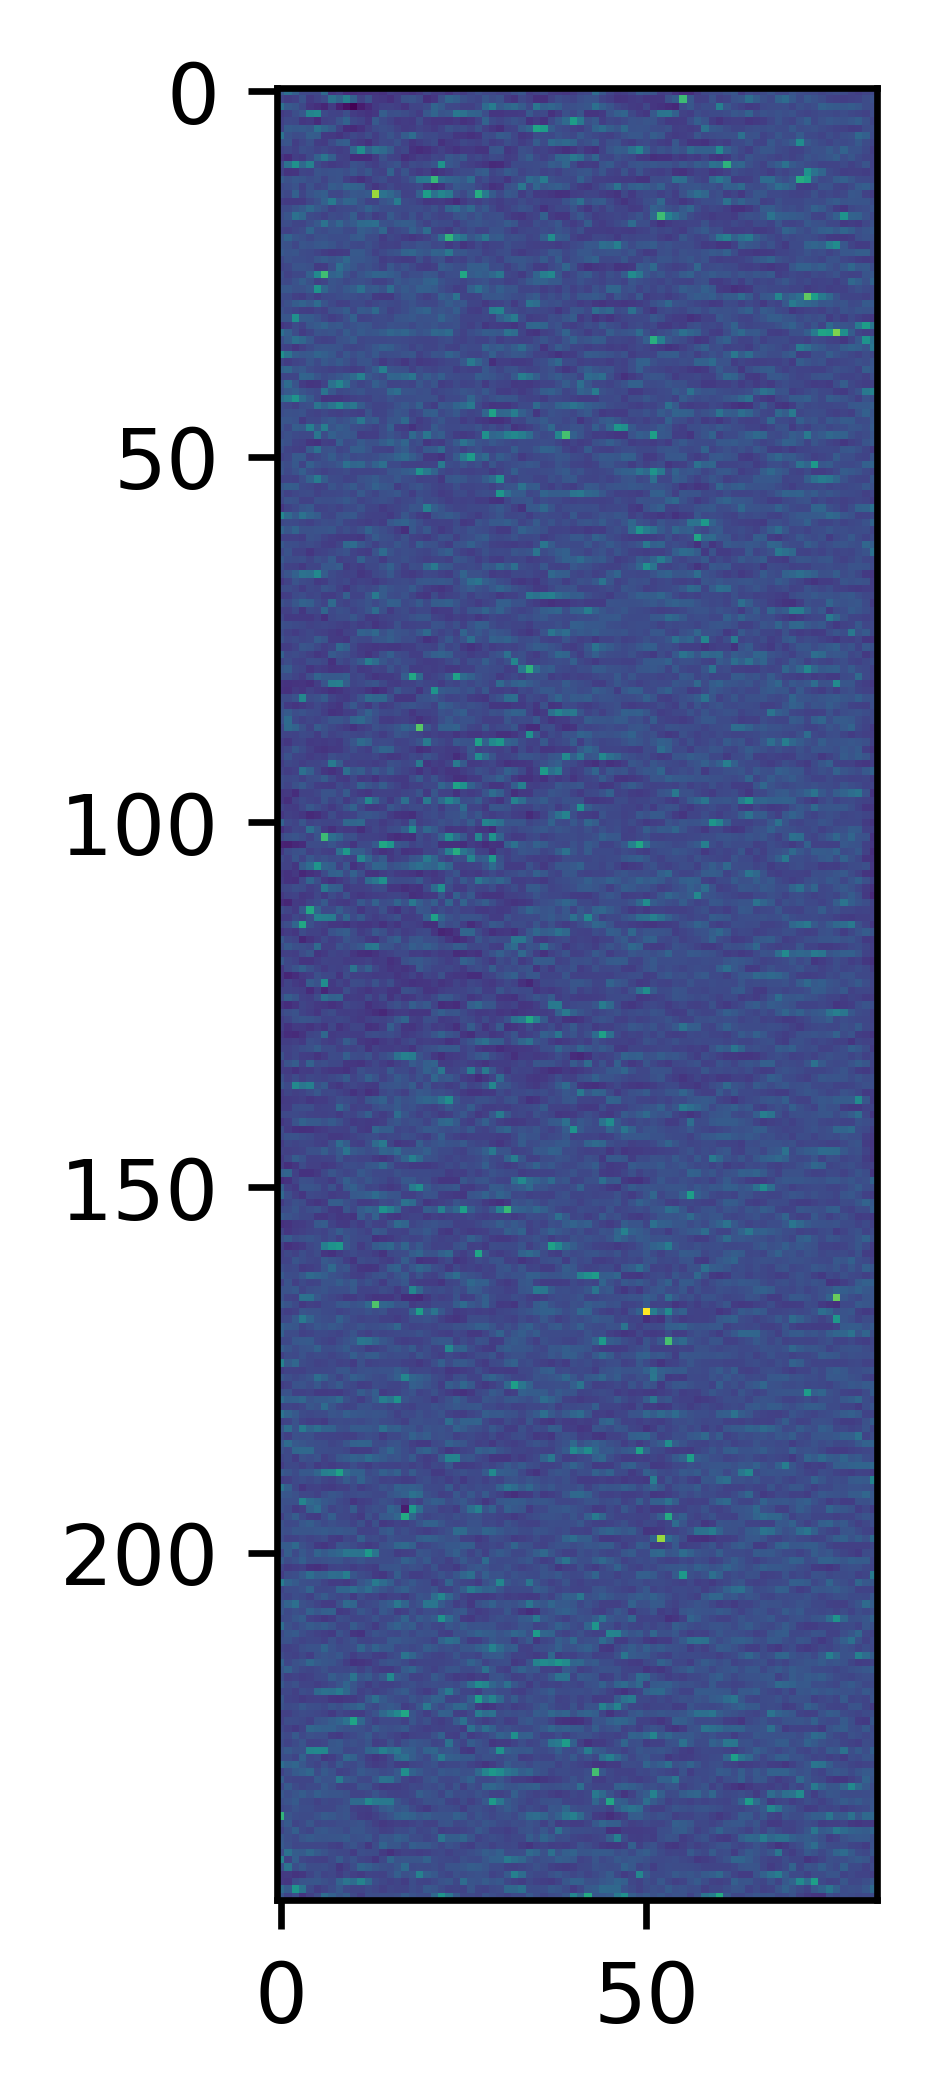
\includegraphics{Graphics/mm-multi-row.png}}
	\subfigure[ ]{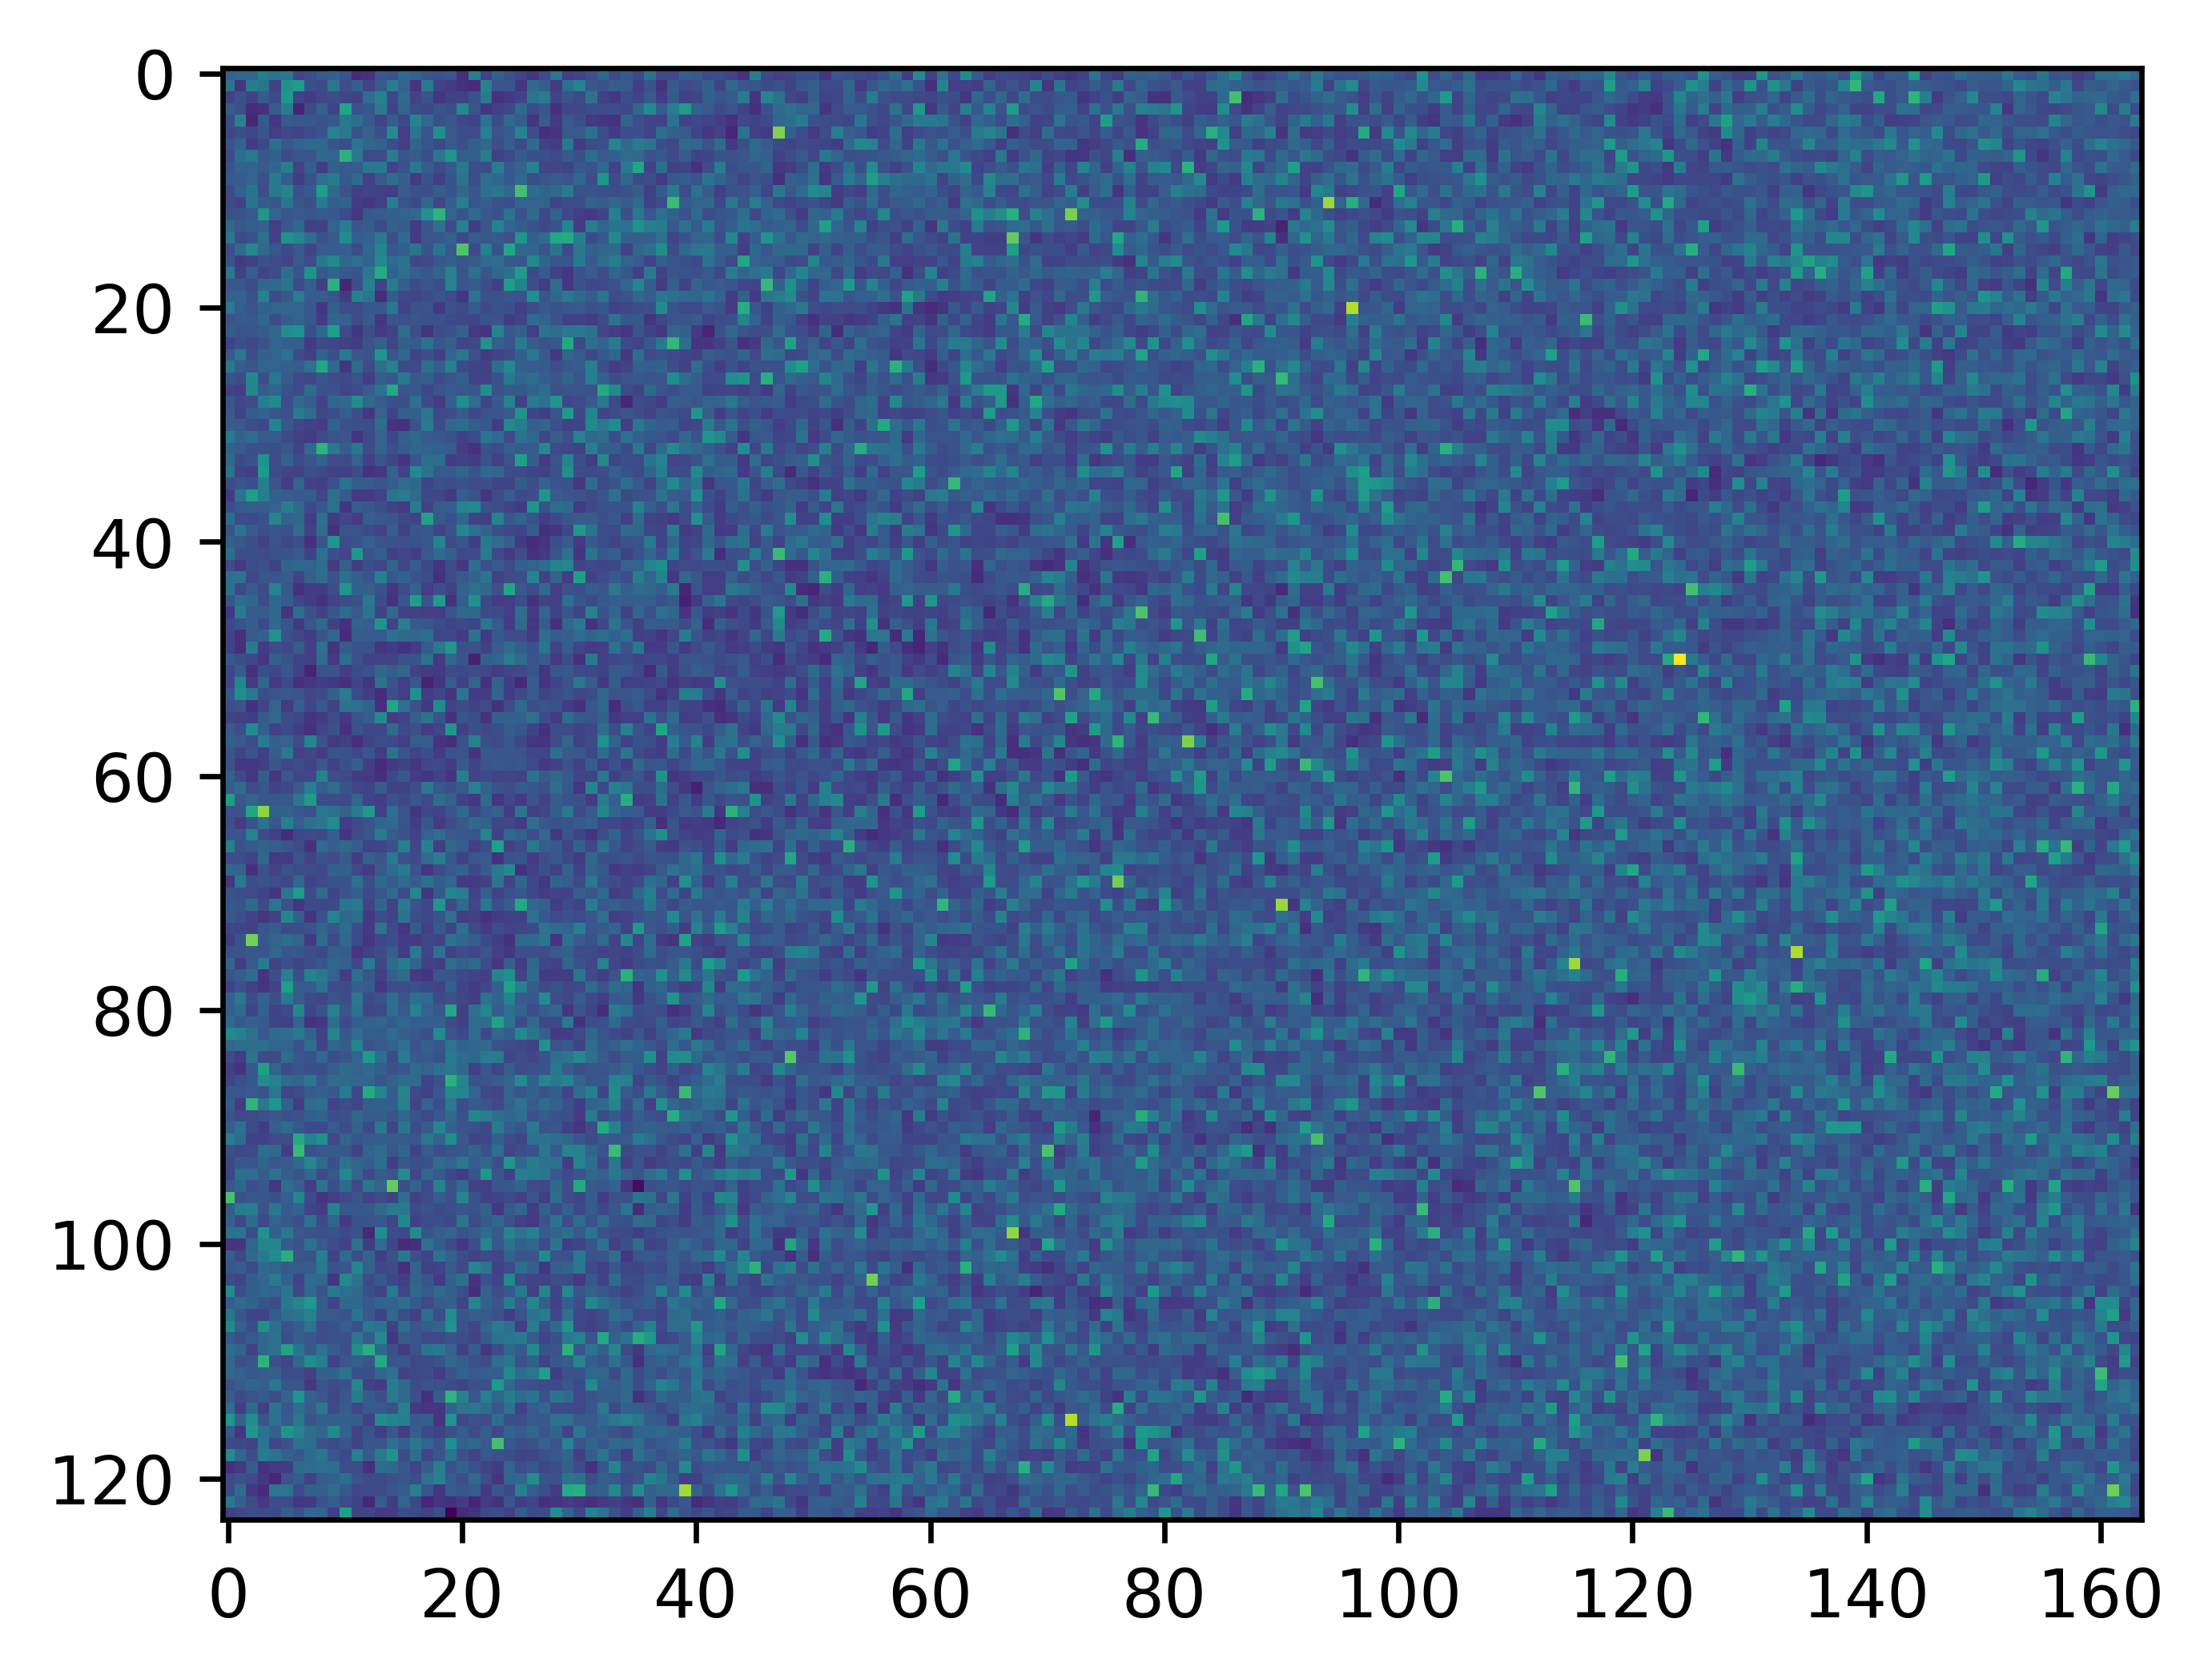
\includegraphics{Graphics/mm-multi-col.png}}
	\caption{} \label{fig:example-mm-approach3}
\end{figure}

El tercer enfoque no logra buenos resultados, tal y como se muestra en la figura \ref{fig:example-mm-approach3}.
No se logra ningún signo de detección y de hecho los valores no superan $0.8$. 


Como conclusión general de los experimentos se puede decir que se logró una replicación exitosa de la DST-II,
y que en el caso unidimensional funcina bastante bien como clasificador para la presencia de un patrón 
dentro de una señal.  Sin embargo, ninguno de los enfoques usados para extender este algoritmo al caso
bidimensional fue fructífero. Aunque el enfoque número dos, lograba hacer detecciones, era a nivel de 
píxeles y sobre una imagen con dimensiones distintas a la original. Esto complica la capacidad de visualizar
dicha detección. Otro problema encontrado durante los experimentos, es que el error de la solución 
del sistema de ecuaciones no lineales es muy importante para que la detección sea exitosa. Si el error
es demasiado alto, entonces el algoritmo no es capaz de diferenciar dentro de la señal la presencia
del patrón. Por último, otro aspecto importante es la sensibilidad ante el ruido del algoritmo. 
Aunque la DST-II logre detectar el patrón, modificaciones del mismo son díficiles de detectar.
En el caso de las masas, su diverso tamaño y forma, no permite que el algoritmo sea capaz de detectarlas
a partir de un único patrón.

